% ============================================================================
% Bitwise AI: A State-of-the-Art Overview
% Main document file
% ============================================================================
\documentclass[11pt,a4paper]{article}

% --- Core packages ---
\usepackage{fontspec}
\usepackage[english]{babel}
\usepackage[top=2.5cm, bottom=2.5cm, left=2.5cm, right=2.5cm]{geometry}

% --- Typography ---
\usepackage{microtype}
\setmainfont{Latin Modern Roman}
\setsansfont{Latin Modern Sans}
\setmonofont{Latin Modern Mono}

% --- Math ---
\usepackage{amsmath, amssymb, amsthm}
\usepackage{mathtools}
\usepackage{bm}

% --- Graphics and diagrams ---
\usepackage{tikz}
\usetikzlibrary{
  arrows.meta, positioning, calc, decorations.pathreplacing,
  shapes.geometric, shapes.misc, fit, backgrounds, patterns,
  matrix, chains, circuits.logic.US
}
\usepackage{pgfplots}
\pgfplotsset{compat=1.18}

% --- Tables and lists ---
\usepackage{booktabs}
\usepackage{tabularx}
\usepackage{enumitem}

% --- Colors ---
\usepackage{xcolor}
\definecolor{bitblue}{HTML}{2563EB}
\definecolor{bitgreen}{HTML}{16A34A}
\definecolor{bitorange}{HTML}{EA580C}
\definecolor{bitpurple}{HTML}{9333EA}
\definecolor{bitgray}{HTML}{6B7280}
\definecolor{lightbg}{HTML}{F8FAFC}

% --- Code and algorithms ---
\usepackage{algorithm}
\usepackage{algpseudocode}

% --- Hyperlinks and references ---
\usepackage[
  colorlinks=true,
  linkcolor=bitblue,
  citecolor=bitgreen,
  urlcolor=bitorange
]{hyperref}
\usepackage[capitalise,noabbrev]{cleveref}

% --- Bibliography ---
\usepackage[
  backend=biber,
  style=numeric-comp,
  sorting=nyt,
  maxbibnames=99
]{biblatex}
\addbibresource{references.bib}

% --- Theorem environments ---
\theoremstyle{definition}
\newtheorem{definition}{Definition}[section]
\newtheorem{example}{Example}[section]
\theoremstyle{remark}
\newtheorem{remark}{Remark}[section]
\theoremstyle{plain}
\newtheorem{theorem}{Theorem}[section]

% --- Custom commands ---
\newcommand{\bitop}[1]{\texttt{\textcolor{bitblue}{#1}}}
\newcommand{\concept}[1]{\textbf{\textcolor{bitpurple}{#1}}}
\newcommand{\xmark}{\textcolor{red}{\ding{55}}}

% --- Custom environments ---
\usepackage{tcolorbox}
\tcbuselibrary{skins, breakable}

\newtcolorbox{keyinsight}[1][]{
  enhanced, breakable,
  colback=bitblue!5, colframe=bitblue!70,
  fonttitle=\bfseries,
  title={Key Insight},
  #1
}

\newtcolorbox{engineernote}[1][]{
  enhanced, breakable,
  colback=bitgreen!5, colframe=bitgreen!70,
  fonttitle=\bfseries,
  title={Engineer's Note},
  #1
}

\newtcolorbox{analogy}[1][]{
  enhanced, breakable,
  colback=bitorange!5, colframe=bitorange!70,
  fonttitle=\bfseries,
  title={Analogy},
  #1
}

% --- Document metadata ---
\title{%
  \textbf{Beyond Multiply-Accumulate}\\[0.5em]
  \Large A Practical Guide to Bitwise Neural Computation\\[0.3em]
  \large An Overview of Four Paradigms for Hardware-Efficient AI
}
\author{Bernhard Gerlach}
\date{March 2026}

% ============================================================================
\begin{document}
% ============================================================================

\maketitle

\begin{abstract}
Modern neural networks are built almost entirely on one operation:
multiply a number by a weight and add the result to a running total.
This \emph{multiply-accumulate} (MAC) operation demands floating-point
hardware, consumes significant energy, and has led to an industry
dominated by GPU manufacturers. But what if neural networks could
be built from the simplest operations a processor can perform---AND,
OR, XOR, and table lookups?

This article surveys four paradigms that pursue this goal:
\textbf{Binary Neural Networks}, which constrain weights to $\{-1, +1\}$
and replace multiplication with XNOR gates;
\textbf{Tsetlin Machines}, which learn propositional logic clauses
through simple automata;
\textbf{Logic Gate Networks}, which learn the wiring \emph{and} type of
logic gates end-to-end; and
\textbf{Kolmogorov-Arnold Networks with Lookup Table compilation},
which train complex learnable functions and then compile them
into memory tables for near-zero-cost inference.

Each paradigm is introduced from first principles, with diagrams
and analogies before equations. The article concludes with a
discussion of how these approaches might be combined into a hybrid
architecture for handwritten digit recognition on the MNIST dataset,
implemented entirely in Rust.
\end{abstract}

\vfill
\tableofcontents
\clearpage

% --- Sections ---
% ============================================================================
\section{Introduction: Why Rethink Neural Computation?}
\label{sec:introduction}
% ============================================================================

Every time you ask a voice assistant a question, every time your phone
recognises a face, every time a language model generates a sentence,
trillions of tiny multiplications happen inside specialised hardware.
These multiplications---floating-point numbers multiplied by
floating-point weights and summed up---are the heartbeat of modern AI.
The industry calls this operation \concept{multiply-accumulate} (MAC),
and virtually every neural network alive today is built on it.

This dependence has consequences---and the industry knows it.
\emph{Quantisation} has become the standard countermeasure: reducing
weights from 32-bit floating-point to 8-bit or even 4-bit integers
cuts memory and energy dramatically. A 70-billion-parameter model
that once required 140\,GB in 16-bit format now fits in roughly
35\,GB at 4~bits (via methods such as GPTQ~\cite{frantar2022gptq} or
AWQ~\cite{lin2023awq}), bringing it within reach of consumer
hardware. Experimental 2-bit quantisation pushes this below 18\,GB.

Yet even aggressively quantised models still rely on integer
multiplication and addition---operations that, while far cheaper than
floating-point, remain significantly more expensive than the simplest
thing a processor can do:

\begin{itemize}[leftmargin=2em]
  \item \textbf{Energy:} At 45\,nm, a 32-bit floating-point
    multiplication costs 3.7\,pJ; an 8-bit integer multiplication costs
    0.2\,pJ---an $18\times$ reduction. But a single bitwise logic
    operation (AND, OR, XOR) costs on the order of 0.1\,pJ, cheaper
    still and $37\times$ below floating-point~\cite{horowitz2014energy}.
    These ratios reflect the algorithmic complexity of each operation
    (a multiplier requires $O(n^2)$ gates, an adder $O(n)$, a bitwise
    operation $O(1)$ per bit) and therefore hold across process
    nodes~\cite{stillmaker2017scaling}.
  \item \textbf{Hardware monopoly:} Training large models still requires
    GPUs, a market dominated by a single manufacturer. Quantised
    inference can run on CPUs, but the underlying matrix multiplications
    over integer values still benefit heavily from specialised
    accelerators.
  \item \textbf{Deployment barriers:} Even with 4-bit quantisation, a
    70-billion-parameter model requires roughly 35\,GB---feasible on a
    high-end laptop but not on a microcontroller, a sensor, or a phone
    without dedicated AI silicon. A fully binary network storing one bit
    per weight would need only $\sim$8\,GB for the same model.
\end{itemize}

\begin{keyinsight}
The question this article explores is not ``How do we build faster
GPUs?'' but rather ``Can we build neural networks that do not need
GPUs at all?''---networks that run on the bitwise logic instructions
every CPU already has.
\end{keyinsight}

\begin{engineernote}
This is a \emph{CPU-first} question, not a claim that a Boolean circuit
automatically runs quickly on a CPU. A useful building block needs packed,
SIMD-friendly data layout, predictable control flow, and local memory
access. The relevant comparison is end-to-end latency and energy against a
small quantised integer baseline on the same processor.
\end{engineernote}

\subsection{The Four Paradigms}

Over the past decade, four distinct research directions have emerged
that aim to replace MAC operations with \emph{bitwise} neural
computation---each attacking the problem from a different angle.
\Cref{fig:paradigm-map} shows how they relate.

\begin{figure}[htbp]
\centering
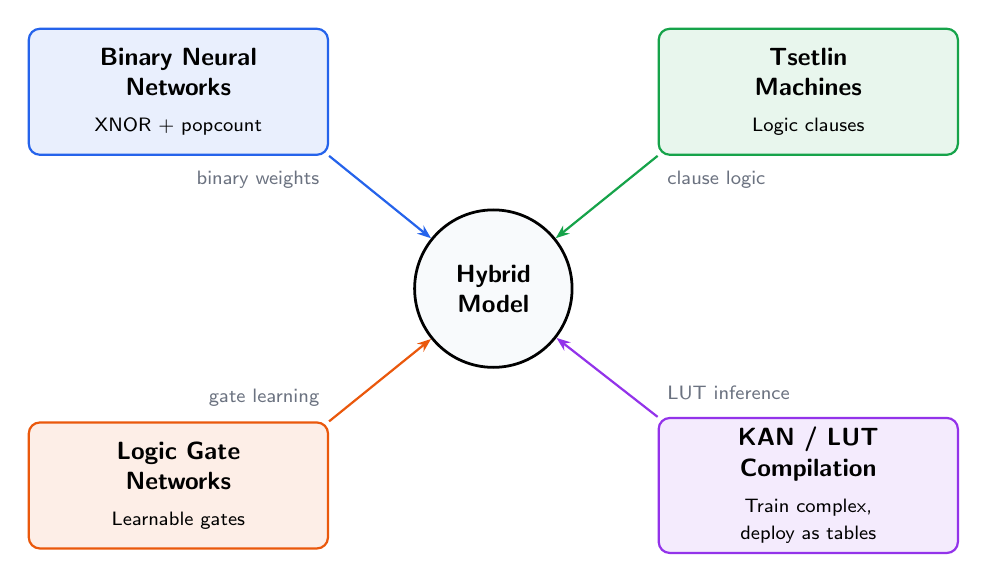
\begin{tikzpicture}[
  box/.style={
    draw, rounded corners=4pt, minimum width=3.8cm, minimum height=1.6cm,
    align=center, font=\small\sffamily, line width=0.8pt
  },
  arrow/.style={-{Stealth[length=5pt]}, thick, bitgray},
  label/.style={font=\scriptsize\sffamily, bitgray}
]
  % Boxes -- wider spacing for readable arrow labels
  \node[box, fill=bitblue!10, draw=bitblue] (bnn)
    at (0,0) {\textbf{Binary Neural}\\\textbf{Networks}\\[2pt]\scriptsize XNOR + popcount};
  \node[box, fill=bitgreen!10, draw=bitgreen] (tm)
    at (8,0) {\textbf{Tsetlin}\\\textbf{Machines}\\[2pt]\scriptsize Logic clauses};
  \node[box, fill=bitorange!10, draw=bitorange] (lgn)
    at (0,-5) {\textbf{Logic Gate}\\\textbf{Networks}\\[2pt]\scriptsize Learnable gates};
  \node[box, fill=bitpurple!10, draw=bitpurple] (kan)
    at (8,-5) {\textbf{KAN / LUT}\\\textbf{Compilation}\\[2pt]\scriptsize Train complex,\\[-1pt]\scriptsize deploy as tables};

  % Central node
  \node[draw, circle, minimum size=2cm, fill=lightbg,
        font=\small\sffamily\bfseries, align=center, line width=1pt]
    (center) at (4,-2.5) {Hybrid\\Model};

  % Arrows to center
  \draw[arrow, bitblue]   (bnn.south east)  -- (center);
  \draw[arrow, bitgreen]  (tm.south west)   -- (center);
  \draw[arrow, bitorange] (lgn.north east)  -- (center);
  \draw[arrow, bitpurple] (kan.north west)  -- (center);

  % Labels on arrows -- horizontal, anchored near the boxes
  \node[label, anchor=east] at ($(bnn.south east)+(0,-0.3)$) {binary weights};
  \node[label, anchor=west] at ($(tm.south west)+(0,-0.3)$) {clause logic};
  \node[label, anchor=east] at ($(lgn.north east)+(0,0.3)$) {gate learning};
  \node[label, anchor=west] at ($(kan.north west)+(0,0.3)$) {LUT inference};
\end{tikzpicture}
\caption{The four paradigms of bitwise neural computation and their
  convergence toward a hybrid architecture. Each contributes a different
  capability: binary arithmetic, interpretable logic, learnable
  structure, and efficient deployment.}
\label{fig:paradigm-map}
\end{figure}

\begin{enumerate}[leftmargin=2em]
  \item \textbf{Binary Neural Networks (BNNs)}~\cite{courbariaux2016bnn} constrain weights and
    sometimes activations to just two values ($+1$ and $-1$). This turns
    multiplication into an XNOR gate and addition into bit-counting
    (\cref{sec:bnn}).
    Proven, fast, but accuracy drops on complex tasks.

  \item \textbf{Tsetlin Machines (TMs)}~\cite{granmo2018tsetlin} abandon the neuron metaphor
    entirely. Instead of weighted sums, they learn \emph{if--then} rules
    (propositional clauses) using simple counting automata
    (\cref{sec:tsetlin}). They achieve
    state-of-the-art results on the MNIST handwritten-digit
    dataset~\cite{lecun1998mnist} while remaining fully
    interpretable.

  \item \textbf{Logic Gate Networks (LGNs)}~\cite{petersen2022difflogic} take a middle path: they
    keep the layered network structure but replace neurons with actual
    logic gates (AND, OR, XOR, etc.). Crucially, the \emph{type} of each
    gate is learned during training through a differentiable relaxation
    (\cref{sec:lgn}).

  \item \textbf{Kolmogorov-Arnold Networks (KANs) with LUT compilation}~\cite{liu2024kan}
    flip the script: train with maximally expressive, learnable
    activation functions (B-spline curves on every edge), then
    \emph{compile} those curves into lookup tables (LUTs) for inference.
    The result is a network that runs on table lookups---pure memory
    access, no arithmetic (\cref{sec:kan}).
\end{enumerate}

\subsection{How to Read This Article}

This article is written for engineers, not mathematicians. Each paradigm
is introduced in three stages:

\begin{enumerate}[leftmargin=2em]
  \item \textbf{Intuition}---an analogy or diagram that conveys the core
    idea without any equations.
  \item \textbf{Mechanism}---how it actually works, with diagrams showing
    data flow and simple numerical examples.
  \item \textbf{Formalization}---the mathematical description, for those
    who want to implement it or read the original papers.
\end{enumerate}

You can read at whatever depth suits you. The intuition sections alone
give a solid understanding; the math sections are there when you need
them.

\subsection{Scope and Goal}

Our concrete starting point is handwritten digit recognition on the
MNIST dataset~\cite{lecun1998mnist}---a 28$\times$28 pixel grayscale
image mapped to one of ten digits (0--9). MNIST is deliberately simple:
the goal is not to set accuracy records but to build a \emph{proof of
concept} that demonstrates bitwise computation can work, implemented
entirely in Rust, benchmarked against a standard floating-point baseline.

Beyond the proof of concept, this article also surveys how each paradigm
can scale. \Cref{sec:transformers-llms} provides a self-contained
introduction to transformers and large language models;
\cref{sec:scaling-llms} evaluates whether every transformer component
can be made integer-only or bitwise; and \cref{sec:hybrid}
sketches a hybrid architecture that combines the best ideas from all
four paradigms.

% ============================================================================
\section{Foundations: From Bits to Neurons}
\label{sec:foundations}
% ============================================================================

Before we can understand how to replace neural network arithmetic with
bitwise operations, we need a shared vocabulary. This section builds the
essential concepts from the ground up.

% ----------------------------------------------------------------------------
\subsection{What a CPU Actually Does Well}
\label{sec:cpu-ops}
% ----------------------------------------------------------------------------

Every processor---from a server CPU to a tiny microcontroller---has
a set of operations it can execute in a single clock cycle. The
cheapest and fastest of these are \concept{bitwise logic operations}:

\begin{figure}[htbp]
\centering
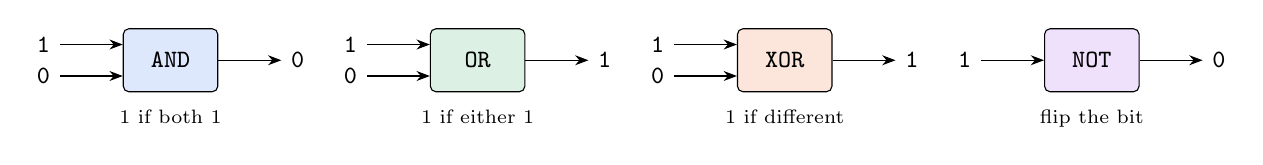
\begin{tikzpicture}[
  gate/.style={draw, minimum width=1.2cm, minimum height=0.8cm,
    font=\small\ttfamily\bfseries, rounded corners=2pt},
  bit/.style={font=\small\ttfamily},
  >=Stealth
]
  % AND gate
  \node[gate, fill=bitblue!15] (and) at (0,0) {AND};
  \node[bit, left=0.8cm] (a1) at ([yshift=0.2cm]and.west) {1};
  \node[bit, left=0.8cm] (a2) at ([yshift=-0.2cm]and.west) {0};
  \node[bit, right=0.8cm] (a3) at (and.east) {0};
  \draw[->] (a1) -- (and.west |- a1);
  \draw[->] (a2) -- (and.west |- a2);
  \draw[->] (and.east) -- (a3);
  \node[font=\scriptsize, below=0.1cm] at (and.south) {1 if both 1};

  % OR gate
  \node[gate, fill=bitgreen!15] (or) at (3.9,0) {OR};
  \node[bit, left=0.8cm] (b1) at ([yshift=0.2cm]or.west) {1};
  \node[bit, left=0.8cm] (b2) at ([yshift=-0.2cm]or.west) {0};
  \node[bit, right=0.8cm] (b3) at (or.east) {1};
  \draw[->] (b1) -- (or.west |- b1);
  \draw[->] (b2) -- (or.west |- b2);
  \draw[->] (or.east) -- (b3);
  \node[font=\scriptsize, below=0.1cm] at (or.south) {1 if either 1};

  % XOR gate
  \node[gate, fill=bitorange!15] (xor) at (7.8,0) {XOR};
  \node[bit, left=0.8cm] (c1) at ([yshift=0.2cm]xor.west) {1};
  \node[bit, left=0.8cm] (c2) at ([yshift=-0.2cm]xor.west) {0};
  \node[bit, right=0.8cm] (c3) at (xor.east) {1};
  \draw[->] (c1) -- (xor.west |- c1);
  \draw[->] (c2) -- (xor.west |- c2);
  \draw[->] (xor.east) -- (c3);
  \node[font=\scriptsize, below=0.1cm] at (xor.south) {1 if different};

  % NOT gate
  \node[gate, fill=bitpurple!15] (not) at (11.7,0) {NOT};
  \node[bit, left=0.8cm] (d1) at (not.west) {1};
  \node[bit, right=0.8cm] (d2) at (not.east) {0};
  \draw[->] (d1) -- (not.west);
  \draw[->] (not.east) -- (d2);
  \node[font=\scriptsize, below=0.1cm] at (not.south) {flip the bit};
\end{tikzpicture}
\caption{The four fundamental logic gates. Each operates on single bits
  and executes in one clock cycle. A 64-bit CPU applies these to 64~bits
  simultaneously.}
\label{fig:logic-gates}
\end{figure}

\begin{engineernote}
When a 64-bit CPU executes an AND instruction, it performs 64
independent AND operations in a single clock cycle. With SIMD
extensions (SSE, AVX-512, NEON), this scales to 128, 256, or even
512~bits at once. This massive parallelism is free---it is built
into the hardware.
\end{engineernote}

There is one more operation that matters enormously: \concept{popcount}
(population count). Given a string of bits, popcount counts how many
are~1. Most modern CPUs have a dedicated popcount instruction.

That instruction is useful, but it is not a universal performance shortcut.
On AVX2 systems, scalar popcount throughput and the absence of a native
vector-popcount instruction can make it a bottleneck in bitwise matrix
multiplication. A recent CPU study improved ternary and binary inference
by fusing packing with quantisation and replacing popcount-heavy kernels
with higher-throughput SIMD operations~\cite{fischer2025popcount}. Bitwise
models therefore need kernel-level measurement, not just operation counts.

\begin{figure}[htbp]
\centering
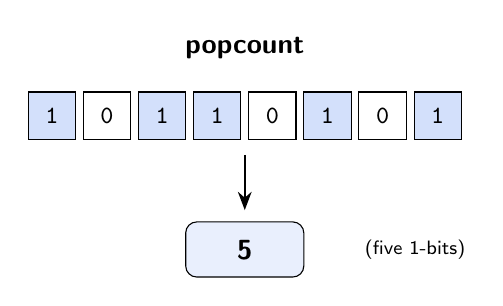
\begin{tikzpicture}[
  bit/.style={draw, minimum width=0.6cm, minimum height=0.6cm,
    font=\small\ttfamily, inner sep=0pt},
  >=Stealth
]
  % Bit string
  \foreach \b [count=\i from 0] in {1,0,1,1,0,1,0,1} {
    \ifnum\b=1
      \def\fillcol{bitblue!20}
    \else
      \def\fillcol{white}
    \fi
    \node[bit, fill=\fillcol]
      (b\i) at (\i*0.7, 0) {\b};
  }
  % Arrow
  \draw[->, thick] (3.5*0.7, -0.5) -- (3.5*0.7, -1.2);
  % Result
  \node[draw, rounded corners, fill=bitblue!10, minimum width=1.5cm,
    minimum height=0.7cm, font=\sffamily\bfseries] at (3.5*0.7, -1.7) {5};
  \node[font=\scriptsize\sffamily, right] at (5.5*0.7, -1.7)
    {(five 1-bits)};
  % Label
  \node[font=\sffamily\bfseries, above=0.3cm] at (3.5*0.7, 0.3)
    {popcount};
\end{tikzpicture}
\caption{The popcount operation counts the number of set bits (1s) in
  a binary word. Combined with XNOR, it becomes a similarity
  measure---see \cref{sec:bnn} for how this replaces multiplication
  in binary neural networks.}
\label{fig:popcount}
\end{figure}

Two more operations round out the bitwise toolkit:
\concept{bit shift} and \concept{bit rotation}. A \emph{left shift}
by $k$ positions moves every bit $k$ places toward the most
significant end, filling the vacated positions with zeros. A
\emph{right shift} does the reverse. Mathematically, shifting left by
$k$ is equivalent to multiplying by $2^k$, and shifting right by $k$
is equivalent to (integer) dividing by $2^k$---but the CPU does it in
a single cycle, without invoking the multiplier or divider circuit.

\begin{figure}[htbp]
\centering
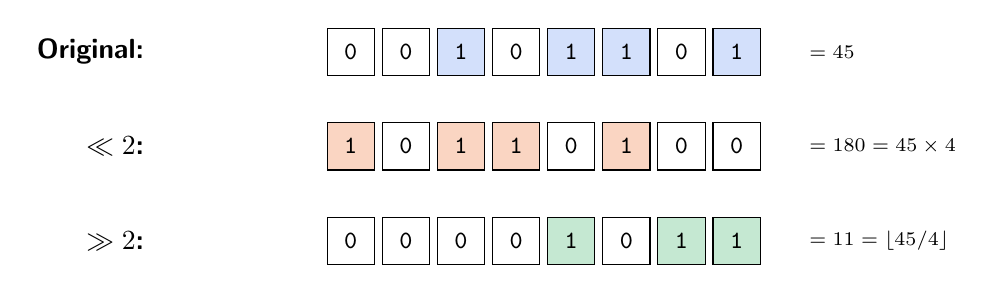
\begin{tikzpicture}[
  bit/.style={draw, minimum width=0.6cm, minimum height=0.6cm,
    font=\small\ttfamily, inner sep=0pt},
  >=Stealth
]
  % Original
  \node[font=\sffamily\bfseries, left] at (-0.5, 0) {Original:};
  \foreach \b [count=\i from 0] in {0,0,1,0,1,1,0,1} {
    \ifnum\b=1
      \def\fillcol{bitblue!20}
    \else
      \def\fillcol{white}
    \fi
    \node[bit, fill=\fillcol] at (\i*0.7+2, 0) {\b};
  }
  \node[font=\scriptsize\sffamily, right] at (7.7, 0) {$= 45$};

  % Left shift by 2
  \node[font=\sffamily\bfseries, left] at (-0.5, -1.2) {$\ll 2$:};
  \foreach \b [count=\i from 0] in {1,0,1,1,0,1,0,0} {
    \ifnum\b=1
      \def\fillcol{bitorange!25}
    \else
      \def\fillcol{white}
    \fi
    \node[bit, fill=\fillcol] at (\i*0.7+2, -1.2) {\b};
  }
  \node[font=\scriptsize\sffamily, right] at (7.7, -1.2)
    {$= 180 = 45 \times 4$};

  % Right shift by 2
  \node[font=\sffamily\bfseries, left] at (-0.5, -2.4) {$\gg 2$:};
  \foreach \b [count=\i from 0] in {0,0,0,0,1,0,1,1} {
    \ifnum\b=1
      \def\fillcol{bitgreen!25}
    \else
      \def\fillcol{white}
    \fi
    \node[bit, fill=\fillcol] at (\i*0.7+2, -2.4) {\b};
  }
  \node[font=\scriptsize\sffamily, right] at (7.7, -2.4)
    {$= 11 = \lfloor 45 / 4 \rfloor$};
\end{tikzpicture}
\caption{Bit shifting. Left shift ($\ll$) multiplies by a power of~2;
  right shift ($\gg$) divides by a power of~2. Both execute in one
  clock cycle. Bit \emph{rotation} is similar but wraps bits around
  instead of discarding them.}
\label{fig:bitshift}
\end{figure}

\begin{engineernote}
Bit shifts turn multiplication and division by powers of~2 into
single-cycle operations. This is why they appear throughout the
integer-only methods in later sections: Shiftmax approximates the
exponential function using shifts (\cref{sec:softmax-problem}),
and integer normalisation replaces square roots and divisions with
iterative shift-and-add sequences
(\cref{sec:layernorm-problem}). Bit \emph{rotation} (wrapping
bits around instead of discarding them) is a standard CPU operation
used in cryptography and hashing but does not currently play a role
in any of the neural network paradigms discussed in this article.
\end{engineernote}

\subsection{The Cost of Arithmetic}
\label{sec:cost-arithmetic}

Not all CPU operations cost the same. \Cref{tab:op-cost} shows
approximate energy costs for different operations in a modern 45\,nm
chip~\cite{horowitz2014energy}.

\begin{table}[htbp]
\centering
\caption{Energy cost of arithmetic operations at a 45\,nm process
  node~\cite{horowitz2014energy}. Modern processors use much smaller
  nodes (5--7\,nm), which lowers \emph{absolute} energies roughly
  5--10$\times$~\cite{stillmaker2017scaling}. However, the \emph{ratios}
  between operation types are determined by algorithmic complexity (a
  multiplier uses $O(n^2)$ gates, an adder $O(n)$, a bitwise operation
  $O(1)$ per bit) and therefore remain approximately constant across
  process generations.}
\label{tab:op-cost}
\begin{tabular}{@{}lrr@{}}
  \toprule
  \textbf{Operation}      & \textbf{Energy (pJ)} & \textbf{Relative Cost} \\
  \midrule
  Bitwise AND/OR/XOR      & 0.1                  & 1$\times$ \\
  Bit shift                & 0.1                  & 1$\times$ \\
  Integer add (8-bit)      & 0.03                 & 0.3$\times$ \\
  Integer multiply (8-bit) & 0.2                  & 2$\times$ \\
  Integer add (32-bit)     & 0.1                  & 1$\times$ \\
  Integer multiply (32-bit)& 3.1                  & 31$\times$ \\
  FP add (32-bit)          & 0.9                  & 9$\times$ \\
  FP multiply (32-bit)     & 3.7                  & 37$\times$ \\
  Memory access (SRAM)     & 5.0                  & 50$\times$ \\
  Memory access (DRAM)     & 640.0                & 6400$\times$ \\
  \bottomrule
\end{tabular}
\end{table}

\begin{keyinsight}
The most expensive thing a chip does is not computation---it is
\emph{moving data}. A DRAM memory access costs 6400$\times$ more
energy than a logic gate. This is the ``memory wall,'' and it means
that any approach which keeps data close to the logic (small models,
local lookups) wins enormously on energy, even if it does more
operations.
\end{keyinsight}

% ----------------------------------------------------------------------------
\subsection{The Precision Spectrum: From 1-Bit to 8-Bit}
\label{sec:precision-spectrum}
% ----------------------------------------------------------------------------

The paradigms in this article differ not only in \emph{which}
operations they use, but in how many bits represent each value.
This distinction is important because it determines what bitwise
operations can meaningfully compute.

\subsubsection{Why Most Approaches Booleanise to 1~Bit}

If every input and every weight is a single bit, then AND, OR, XOR,
and NOT are the \emph{natural} operations---they map exactly onto
the logic of combining two Boolean propositions. XNOR on two 1-bit
values tells you whether they agree. Popcount on a vector of XNOR
results tells you how many positions agree---a Hamming
similarity.\footnote{The \emph{Hamming distance} between two binary
strings is the number of positions at which the bits differ. It was
introduced by Richard Hamming in~1950 for error-detecting codes.
\emph{Hamming similarity} is the complement: the number of positions
that \emph{agree}. For two $n$-bit strings $a$ and~$b$:
$\text{similarity} = n - \text{distance}
= \operatorname{popcount}(\operatorname{XNOR}(a,b))$.}
This is maximally hardware-efficient: a 64-bit CPU processes 64
independent 1-bit operations in a single instruction.

The price is \concept{precision loss}. For MNIST, collapsing each
pixel to 1~bit (ink or background) loses surprisingly little
information---the images are nearly binary already. But for richer
inputs (colour images, audio spectrograms, word embeddings),
reducing to 1~bit per feature is destructive.

\subsubsection{The Positional Encoding Problem}

Why not simply apply XNOR to 8-bit values? You can---but the
result is not what you might expect. An 8-bit integer stores its
value in \emph{positional binary encoding}: bit~7 is worth~128,
bit~0 is worth~1. Bitwise operations treat all bit positions
identically---they do not know that bit~7 matters 128$\times$ more
than bit~0.

\begin{analogy}
Applying XOR to two 8-bit integers is like comparing two
five-digit numbers by checking how many \emph{digits} match,
regardless of position. The numbers 50{,}001 and 50{,}002 differ
in one digit (the units), but so do 50{,}001 and 10{,}001 (the
ten-thousands). Position-blind comparison treats these as equally
different, even though the first pair is numerically close and the
second pair is far apart.
\end{analogy}

To make bitwise operations numerically meaningful on multi-bit
values, you need one of three approaches:

\begin{enumerate}[leftmargin=2em]
  \item \textbf{Carry propagation}---let the result of one bit
    position influence the next. This is exactly what integer
    addition does: it is implemented as a chain of XOR gates (for
    the sum bits) and AND gates (for the carries). In other words,
    integer addition \emph{is} a structured sequence of bitwise
    operations with inter-bit dependencies.

  \item \textbf{Unary (thermometer) encoding}---represent the
    value~5 not as \texttt{0101} but as \texttt{11111000} (five~1s
    followed by zeros). Now bitwise AND gives the minimum of two
    values, OR gives the maximum, and Hamming distance correlates
    with numerical distance. The cost: a $k$-bit value becomes a
    $(2^k - 1)$-bit thermometer, a large expansion.

  \item \textbf{Accept the approximation}---use Hamming distance on
    raw binary as a rough similarity measure. This works
    surprisingly well when combined with large vectors and
    averaging (high-dimensional statistics smooth out the
    positional noise).
\end{enumerate}

\subsubsection{The Precision--Operation Map}

\Cref{tab:precision-map} shows how different approaches in this
article combine data precision with operation types. The field has
split into two camps: \emph{pure logic} (1-bit data, logic gates)
and \emph{integer quantisation} (multi-bit data, integer arithmetic).

\begin{table}[htbp]
\centering
\caption{The precision spectrum. Approaches differ in how many bits
  represent data and weights, which determines what operations are
  efficient.}
\label{tab:precision-map}
\small
\begin{tabular}{@{}p{2.6cm}ccp{3.7cm}l@{}}
  \toprule
  \textbf{Approach} & \textbf{Data} & \textbf{Weights}
    & \textbf{Core operations} & \textbf{Used by} \\
  \midrule
  Full binary
    & 1 bit & 1 bit
    & AND, OR, XOR, NOT
    & BNN, TM, LGN \\[3pt]
  Thermometer
    & $k$ bits (unary) & 1 bit
    & Logic on expanded features
    & Advanced TM \\[3pt]
  Ternary weights
    & 8 bit & 1.58 bit
    & Integer add/subtract
    & BitNet b1.58 \\[3pt]
  Low-bit integer
    & 4--8 bit & 4--8 bit
    & Integer + bit shifts
    & I-BERT, I-ViT \\[3pt]
  LUT deployment
    & any & (compiled)
    & Memory read
    & KAN/LUT, ULEEN \\
  \bottomrule
\end{tabular}
\end{table}

\begin{keyinsight}
Notice the gap in \cref{tab:precision-map}: \textbf{no approach
combines multi-bit data with pure bitwise operations (no integer
addition).} The ``pure logic'' camp booleanises everything to 1~bit;
the ``integer'' camp keeps multi-bit data but relies on integer
addition with carry propagation. The middle ground---multi-bit data
processed only with shifts, masks, and position-independent logic---is
largely unexplored. Whether novel encodings (thermometer, Gray code,
or something entirely new) could make this viable is an open research
question. Classical integer addition costs $9\times$ the energy of a
bitwise operation (\cref{tab:op-cost}); if it could be avoided while
retaining multi-bit precision, the efficiency gain would be
significant.
\end{keyinsight}

% ----------------------------------------------------------------------------
\subsection{How a Traditional Neuron Works}
\label{sec:traditional-neuron}
% ----------------------------------------------------------------------------

A single artificial neuron does three things:

\begin{enumerate}[leftmargin=2em]
  \item \textbf{Multiply} each input $x_i$ by a learned weight $w_i$.
  \item \textbf{Accumulate} (sum) all the products and add a bias $b$.
  \item \textbf{Activate} by passing the sum through a nonlinear function $\sigma$.
\end{enumerate}

\begin{equation}
  y = \sigma\!\left(\sum_{i=1}^{n} w_i \cdot x_i + b\right)
  \label{eq:neuron}
\end{equation}

\begin{figure}[htbp]
\centering
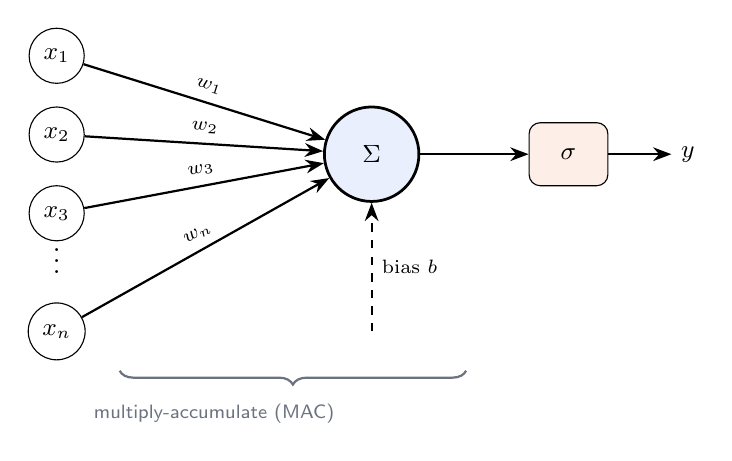
\begin{tikzpicture}[
  input/.style={circle, draw, minimum size=0.7cm, font=\small},
  neuron/.style={circle, draw, minimum size=1.2cm, font=\small,
    fill=bitblue!10, line width=1pt},
  >=Stealth
]
  % Inputs
  \foreach \i/\v in {1/x_1, 2/x_2, 3/x_3} {
    \node[input] (in\i) at (0, 2-\i) {$\v$};
  }
  \node at (0, -1.5) {$\vdots$};
  \node[input] (inn) at (0, -2.5) {$x_n$};

  % Neuron
  \node[neuron] (n) at (4, -0.25) {$\Sigma$};

  % Activation
  \node[draw, rounded corners, minimum width=1cm, minimum height=0.8cm,
    fill=bitorange!10, font=\small] (act) at (6.5, -0.25) {$\sigma$};

  % Output
  \node[right=0.8cm, font=\small] (out) at (act.east) {$y$};

  % Connections with weights
  \foreach \i in {1,2,3} {
    \draw[->, thick] (in\i) -- node[above, font=\scriptsize, sloped]
      {$w_\i$} (n);
  }
  \draw[->, thick] (inn) -- node[above, font=\scriptsize, sloped]
    {$w_n$} (n);

  % Neuron to activation
  \draw[->, thick] (n) -- (act);
  \draw[->, thick] (act) -- (out);

  % Bias
  \draw[->, thick, dashed] (4, -2.5) -- node[right, font=\scriptsize]
    {bias $b$} (n);

  % Labels
  \node[font=\scriptsize\sffamily, below=0.1cm, bitgray] at (2, -3.2)
    {multiply-accumulate (MAC)};
  \draw[decorate, decoration={brace, amplitude=5pt, mirror},
    bitgray, thick] (0.8, -3) -- (5.2, -3);
\end{tikzpicture}
\caption{A traditional artificial neuron. The multiply-accumulate step
  dominates both computation time and energy cost. Every paradigm in
  this article replaces this step with something cheaper.}
\label{fig:traditional-neuron}
\end{figure}

\begin{analogy}
Think of a neuron as a judge at a talent show. Each judge gives a
score (the input $x_i$), and each judge has a reputation weight
($w_i$)---a famous expert's opinion counts more. The final score is
the weighted average. The activation function is the threshold: above
a certain score, the act goes through; below, it is rejected.

The MAC approach computes this weighted average with precise
floating-point arithmetic. The bitwise approaches we will explore
are like replacing the nuanced scoring with a simpler system:
thumbs-up or thumbs-down from each judge, then just counting votes.
\end{analogy}

% ----------------------------------------------------------------------------
\subsection{What MNIST Looks Like}
\label{sec:mnist}
% ----------------------------------------------------------------------------

The MNIST dataset~\cite{lecun1998mnist} is the standard first benchmark
for any new neural network approach. It consists of 70,000 handwritten
digit images (60,000 for training, 10,000 for testing), each
28$\times$28 pixels in grayscale (values 0--255).

\begin{figure}[htbp]
\centering
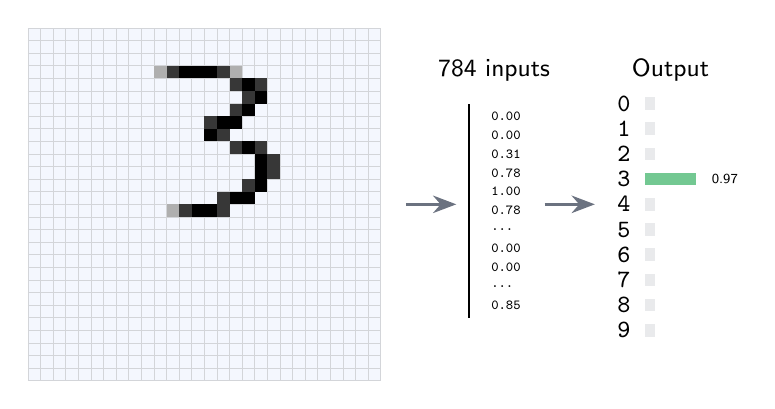
\begin{tikzpicture}[scale=0.16]
  % Draw a stylised "3" as a pixel grid
  \fill[bitblue!5] (0,0) rectangle (28,28);
  \draw[bitgray!30, very thin, step=1] (0,0) grid (28,28);

  % Approximate pixels for digit "3"
  \foreach \x/\y/\c in {
    10/24/80, 11/24/200, 12/24/255, 13/24/255, 14/24/255, 15/24/200, 16/24/80,
    16/23/200, 17/23/255, 18/23/200,
    17/22/200, 18/22/255,
    16/21/200, 17/21/255,
    14/20/200, 15/20/255, 16/20/255,
    14/19/255, 15/19/200,
    16/18/200, 17/18/255, 18/18/200,
    18/17/255, 19/17/200,
    18/16/255, 19/16/200,
    17/15/200, 18/15/255,
    15/14/200, 16/14/255, 17/14/255,
    11/13/80, 12/13/200, 13/13/255, 14/13/255, 15/13/200
  }{
    \pgfmathsetmacro{\intensity}{\c/255*100}
    \fill[black!\intensity] (\x,\y) rectangle ++(1,1);
  }

  % Arrow
  \draw[-{Stealth}, very thick, bitgray] (30, 14) -- (34, 14);

  % Vector representation
  \node[font=\small\sffamily, anchor=south] at (37, 23) {784 inputs};
  \draw[thick] (35, 5) -- (35, 22);
  \foreach \y/\v in {21/0.00, 19.5/0.00, 18/0.31, 16.5/0.78, 15/1.00,
    13.5/0.78, 12/\ldots, 10.5/0.00, 9/0.00, 7.5/\ldots, 6/0.85} {
    \node[font=\tiny\ttfamily, right] at (36, \y) {\v};
  }

  % Arrow to output
  \draw[-{Stealth}, very thick, bitgray] (41, 14) -- (45, 14);

  % Output
  \node[font=\small\sffamily, anchor=south] at (51, 23) {Output};
  \foreach \d [count=\i from 0] in {0,1,2,3,4,5,6,7,8,9} {
    \pgfmathsetmacro{\ypos}{22 - \i * 2.0}
    \node[font=\small\ttfamily, right] at (46, \ypos) {\d};
    \ifnum\d=3
      \fill[bitgreen!60] (49, {\ypos-0.5}) rectangle (53, {\ypos+0.5});
      \node[font=\tiny\sffamily, right] at (53.5, \ypos) {0.97};
    \else
      \fill[bitgray!15] (49, {\ypos-0.5}) rectangle (49.8, {\ypos+0.5});
    \fi
  }
\end{tikzpicture}
\caption{The MNIST task: a 28$\times$28 grayscale image is flattened
  into 784 values (normalised to $[0,1]$), and the network must output
  which digit (0--9) it represents. The standard floating-point
  baseline achieves 98--99\% accuracy.}
\label{fig:mnist}
\end{figure}

For bitwise networks, the first question is how to represent these
pixel values as bits. The simplest approach is \concept{thresholding}:
if a pixel is above 127, it becomes a~1; otherwise a~0. More
sophisticated approaches use \concept{thermometer encoding} (multiple
bits per pixel) or learned binarisation~\cite{lab2023}. We will revisit this in each
paradigm's section.

% ----------------------------------------------------------------------------
\subsection{What ``Training'' Means}
\label{sec:training-overview}
% ----------------------------------------------------------------------------

Training a neural network means adjusting its parameters (weights,
thresholds, gate types, spline coefficients---depending on the paradigm)
so that the network's outputs match the \emph{known correct answers} in
a labelled training set. This is \concept{supervised learning}: each
training example comes with the right answer (e.g.\ an image of a~3
paired with the label ``3''), and the network learns by comparing its
prediction to that label. In traditional networks, this comparison-and-correction
cycle uses \concept{gradient descent}:

\begin{enumerate}[leftmargin=2em]
  \item Run inputs through the network (\emph{forward pass}).
  \item Measure how wrong the output is by comparing it to the known
    correct answer---this score is called the \emph{loss}.
  \item Compute how each parameter contributed to the error
    (\emph{backward pass / backpropagation}).
  \item Nudge each parameter a tiny step in the direction that
    reduces the error.
\end{enumerate}

\begin{engineernote}
Backpropagation works by applying the chain rule of calculus: starting
from the loss, it computes the derivative of each layer's output with
respect to that layer's parameters, then chains these derivatives
together to propagate the error signal all the way back to the first
layer. This requires that every operation in the network be
\emph{differentiable}---that we can compute how a tiny change in its
input affects its output. Logic gates (AND, OR, XOR) are \emph{not}
differentiable: their output jumps discretely from~0 to~1 with no
smooth transition, so the derivative is either zero or undefined. This
is the central challenge of bitwise neural networks, and each paradigm
solves it differently:
\begin{itemize}[leftmargin=1em]
  \item BNNs use the ``straight-through estimator''~\cite{bengio2013ste}---pretend the
    derivative exists (\cref{sec:bnn}).
  \item Tsetlin Machines~\cite{granmo2018tsetlin} avoid gradients entirely, using
    \emph{reinforcement learning}---a training paradigm where each
    component receives simple reward/penalty signals (``that clause
    was useful'' or ``that clause was not'') and adjusts its behaviour
    accordingly, with no derivatives required (\cref{sec:tsetlin}).
  \item LGNs~\cite{petersen2022difflogic} use a continuous relaxation that converges to discrete
    gates (\cref{sec:lgn}).
  \item KANs train in continuous space and discretise only at
    deployment (\cref{sec:kan}).
\end{itemize}
\end{engineernote}

With this foundation, we are ready to explore each paradigm in detail.

% ============================================================================
\section{Paradigm 1: Binary Neural Networks}
\label{sec:bnn}
% ============================================================================

% --- Intuition ---
\subsection{The Idea in Plain English}

Imagine you have a row of light switches, each either on or off. Now
imagine a second row---a ``template'' of the ideal pattern for the
digit~3. To check how well they match, you simply compare them
switch by switch: same position = match, different position = mismatch.
Count the matches, and you have a similarity score. No multiplication
needed.

This is exactly what a Binary Neural Network does~\cite{courbariaux2016bnn}. It forces both the
inputs and the weights to be binary ($+1$ or $-1$), then measures
similarity using \bitop{XNOR} (same = 1, different = 0) and
\bitop{popcount} (count the 1s).

\begin{analogy}
If a traditional neuron is a panel of judges giving scores from 1 to
10 and computing a weighted average, a binary neuron is a panel voting
yes/no and counting hands. You lose nuance, but the counting is
\emph{incredibly} fast.
\end{analogy}

% --- Mechanism ---
\subsection{How It Works}

\subsubsection{Step 1: Binarise the Weights}

During training, the network maintains full-precision (32-bit floating
point) ``shadow'' weights. At each forward pass, these are snapped to
binary using the sign function:

\begin{equation}
  w_b = \operatorname{sign}(w) =
  \begin{cases}
    +1 & \text{if } w \geq 0 \\
    -1 & \text{if } w < 0
  \end{cases}
  \label{eq:sign}
\end{equation}

\subsubsection{Step 2: Binarise the Inputs}

Similarly, activations (layer outputs) are binarised. For MNIST, the
raw pixels can be thresholded directly: pixel value $> 127$ becomes
$+1$, otherwise $-1$.

\subsubsection{Step 3: Replace Multiply with XNOR}

The key mathematical identity that makes BNNs work:

\begin{keyinsight}
When both operands are in $\{-1, +1\}$, multiplication is equivalent
to the XNOR operation:
\[
  a \cdot b = \operatorname{XNOR}(a, b) \quad
  \text{where } +1 \leftrightarrow 1, \quad -1 \leftrightarrow 0
\]
Two values that are the same multiply to $+1$ (XNOR = 1); two
values that differ multiply to $-1$ (XNOR = 0).

Why XNOR and not XOR? Because we want a \emph{similarity} measure:
positions where input and weight agree should contribute~$+1$ to the
sum, and positions where they disagree should contribute~$-1$. XNOR
returns~1 when both bits are equal (same = match), which is exactly
the right semantics. XOR does the opposite---it returns~1 when bits
\emph{differ}, so it would give a \emph{dis}similarity count.
\end{keyinsight}

\subsubsection{Step 4: Replace Sum with Popcount}

The sum of $n$ XNOR results (each 0 or~1) equals the number of
matches. If $p$ is the popcount and $n$ is the total number of bits:
\begin{equation}
  \sum_{i=1}^{n} w_i \cdot x_i = 2 \cdot \operatorname{popcount}
    (\operatorname{XNOR}(\bm{w}, \bm{x})) - n
  \label{eq:xnor-popcount}
\end{equation}

\begin{figure}[htbp]
\centering
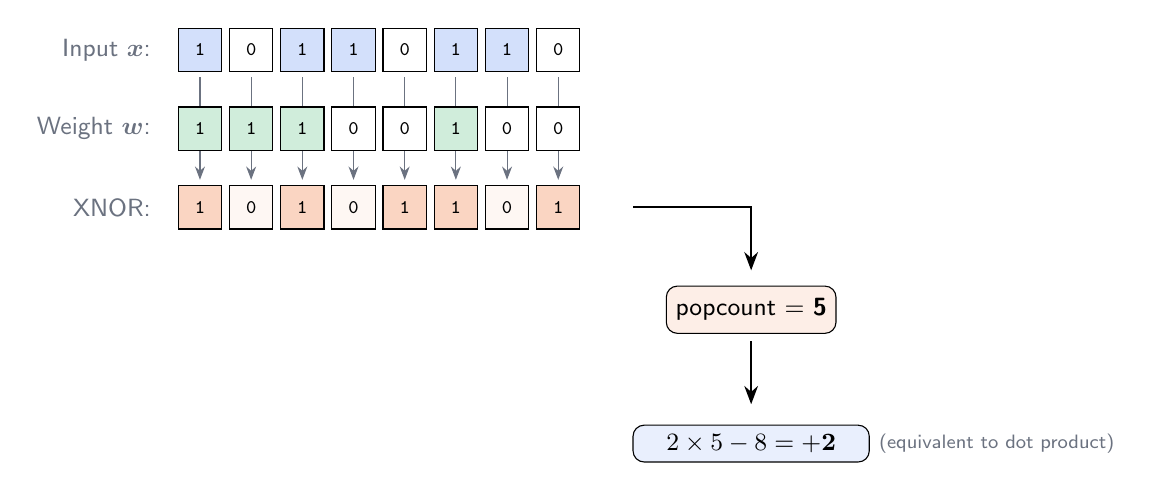
\begin{tikzpicture}[
  bit/.style={draw, minimum width=0.55cm, minimum height=0.55cm,
    font=\scriptsize\ttfamily, inner sep=0pt},
  lbl/.style={font=\small\sffamily, bitgray},
  >=Stealth
]
  % Input bits
  \node[lbl, left] at (-0.5, 2) {Input $\bm{x}$:};
  \foreach \b [count=\i from 0] in {1,0,1,1,0,1,1,0} {
    \ifnum\b=1
      \def\fillcol{bitblue!20}
    \else
      \def\fillcol{white}
    \fi
    \node[bit, fill=\fillcol]
      (x\i) at (\i*0.65, 2) {\b};
  }

  % Draw comparison arrows first so the filled bit boxes mask the shafts.
  \foreach \i in {0,...,7} {
    \draw[->, thin, bitgray] (\i*0.65, 1.65) -- (\i*0.65, 0.35);
  }

  % Weight bits
  \node[lbl, left] at (-0.5, 1) {Weight $\bm{w}$:};
  \foreach \b [count=\i from 0] in {1,1,1,0,0,1,0,0} {
    \ifnum\b=1
      \def\fillcol{bitgreen!20}
    \else
      \def\fillcol{white}
    \fi
    \node[bit, fill=\fillcol]
      (w\i) at (\i*0.65, 1) {\b};
  }

  % XNOR result
  \node[lbl, left] at (-0.5, 0) {XNOR:};
  \foreach \b [count=\i from 0] in {1,0,1,0,1,1,0,1} {
    \ifnum\b=1
      \def\fillcol{bitorange!25}
    \else
      \def\fillcol{bitorange!5}
    \fi
    \node[bit, fill=\fillcol]
      (r\i) at (\i*0.65, 0) {\b};
  }

  % Popcount
  \draw[->, thick] (5.5, 0) -- (7, 0) -- (7, -0.8);
  \node[draw, rounded corners, fill=bitorange!10, minimum width=2cm,
    minimum height=0.6cm, font=\small\sffamily] (pc) at (7, -1.3)
    {popcount = \textbf{5}};

  % Final result
  \draw[->, thick] (7, -1.7) -- (7, -2.5);
  \node[draw, rounded corners, fill=bitblue!10, minimum width=3cm,
    font=\small\sffamily] at (7, -3)
    {$2 \times 5 - 8 = \mathbf{+2}$};

  % Annotation
  \node[font=\scriptsize\sffamily, bitgray, right] at (8.5, -3)
    {(equivalent to dot product)};
\end{tikzpicture}
\caption{A binary neuron in action. Eight input bits are compared with
  eight weight bits using XNOR. The popcount of the result (5 matches
  out of 8) is converted to a signed dot product: $2 \times 5 - 8 = +2$.
  On a 64-bit CPU, this processes 64~inputs in two instructions.}
\label{fig:bnn-computation}
\end{figure}

% --- Training ---
\subsection{The Training Problem and the Straight-Through Estimator}

The sign function (\cref{eq:sign}) has zero derivative almost
everywhere and is undefined at zero. This means backpropagation
cannot flow through it---gradients vanish.

The pragmatic solution is the \concept{straight-through estimator}
(STE)~\cite{bengio2013ste}: during the backward pass, \emph{pretend}
the sign function is the identity function ($\frac{\partial w_b}
{\partial w} \approx 1$). In other words, the sign function has a
true derivative of~0 almost everywhere (the output is flat at~$+1$ or
flat at~$-1$, so a tiny change in the input changes nothing in the
output). The STE simply replaces this useless zero with a gradient
of~1, as if the binarisation step were not there. The error signal
from later layers passes straight through the sign function unchanged,
and the full-precision shadow weights are updated normally. Yes, this
is mathematically unjustified---but it works well enough in practice.

\begin{figure}[htbp]
\centering
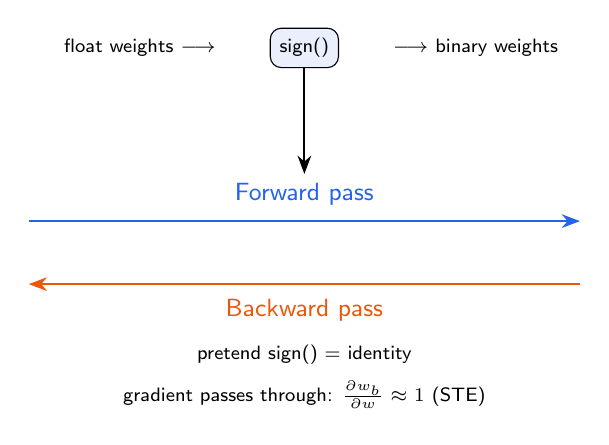
\begin{tikzpicture}[>=Stealth]
  % Forward pass arrow
  \draw[->, thick, bitblue] (0, -0.7) -- (7, -0.7);
  \node[font=\small\sffamily, bitblue, above=2pt] at (3.5, -0.7) {Forward pass};

  % Sign box above the line
  \node[draw, fill=bitblue!10, rounded corners, font=\scriptsize\sffamily,
    minimum height=0.5cm] (signbox) at (3.5, 1.5) {sign()};
  \draw[->, thick] (signbox.south) -- (3.5, -0.1);

  % Labels left and right of sign box
  \node[font=\scriptsize\sffamily, anchor=east] at (2.5, 1.5)
    {float weights $\longrightarrow$};
  \node[font=\scriptsize\sffamily, anchor=west] at (4.5, 1.5)
    {$\longrightarrow$ binary weights};

  % Backward pass arrow
  \draw[<-, thick, bitorange] (0, -1.5) -- (7, -1.5);
  \node[font=\small\sffamily, bitorange, below=2pt] at (3.5, -1.5)
    {Backward pass};

  % STE explanation below
  \node[font=\scriptsize\sffamily] at (3.5, -2.4)
    {pretend sign() = identity};
  \node[font=\scriptsize\sffamily] at (3.5, -2.9)
    {gradient passes through: $\frac{\partial w_b}{\partial w} \approx 1$
    (STE)};
\end{tikzpicture}
\caption{The straight-through estimator: use binary weights going
  forward, but let gradients flow as if the binarisation step was not
  there during backpropagation.}
\label{fig:ste}
\end{figure}

This is a hack, and it introduces noise into the gradient signal. But
it works well enough to train BNNs to useful accuracy levels.

% --- Formalisation ---
\subsection{Mathematical Summary}
\label{sec:bnn-math}

A binary linear layer with $m$ inputs and $n$ outputs is defined as
follows. Here $\bm{W} \in \mathbb{R}^{n \times m}$ is the matrix of
full-precision shadow weights (one row per output neuron, one column
per input), and $\bm{x} \in \mathbb{R}^m$ is the input vector:

\begin{align}
  \bm{W}_b &= \operatorname{sign}(\bm{W}) \in \{-1, +1\}^{n \times m}
    & &\text{(binarise weights)}
    \label{eq:bnn-weight} \\
  \bm{x}_b &= \operatorname{sign}(\bm{x}) \in \{-1, +1\}^m
    & &\text{(binarise inputs)}
    \label{eq:bnn-input} \\
  \bm{z} &= \bm{W}_b \bm{x}_b
    = 2 \cdot \operatorname{popcount}(\operatorname{XNOR}(\bm{W}_b, \bm{x}_b)) - m
    & &\text{(forward pass)}
    \label{eq:bnn-forward} \\
  \bm{y} &= \operatorname{BatchNorm}(\bm{z})
    & &\text{(normalise)}
    \label{eq:bnn-output}
\end{align}

\Cref{eq:bnn-forward} is the key line. The product $\bm{W}_b \bm{x}_b$
is a standard matrix-vector multiply, but because both operands are in
$\{-1,+1\}$, each scalar multiply $w_i \cdot x_i$ is either~$+1$ (if
they agree) or~$-1$ (if they differ). Encoding $+1$ as bit~1 and $-1$
as bit~0, this becomes an XNOR. The sum of all $m$ products equals
the number of agreements minus the number of disagreements. Since
$\text{agreements} = \operatorname{popcount}$ and
$\text{disagreements} = m - \operatorname{popcount}$, the total is
$\operatorname{popcount} - (m - \operatorname{popcount})
= 2 \cdot \operatorname{popcount} - m$.

\concept{Batch normalisation} (\cref{eq:bnn-output}) is a technique
that re-centres and re-scales a layer's outputs so they have
approximately zero mean and unit variance across a batch of training
examples. In BNNs this is critical: without it, the integer-valued
popcount outputs would drift and cluster, and the next binarisation
step (sign function) would collapse most values to the same sign,
destroying information. Unfortunately, batch normalisation involves
floating-point division and square roots, making it the main
remaining non-bitwise operation in a BNN.

\subsection{Performance on MNIST and Beyond}
\label{sec:bnn-performance}

\begin{table}[htbp]
\centering
\caption{BNN performance benchmarks from the literature~\cite{courbariaux2016bnn, rastegari2016xnornet, bnnfpga2025, ma2024bitnet}. BitNet b1.58's ternary approach is analysed in detail in \cref{sec:bitnet-reality}.}
\label{tab:bnn-perf}
\begin{tabular}{@{}llrr@{}}
  \toprule
  \textbf{Architecture} & \textbf{Dataset} & \textbf{Accuracy} & \textbf{Speedup} \\
  \midrule
  BNN~\cite{courbariaux2016bnn} & MNIST   & 98.6\%  & 7$\times$ \\
  XNOR-Net~\cite{rastegari2016xnornet} & ImageNet & 51.2\%  & 58$\times$ \\
  BNN on FPGA~\cite{bnnfpga2025} & MNIST   & 84.0\%  & Real-time \\
  BitNet b1.58~\cite{ma2024bitnet} & LLM 3B  & Competitive & 2.7$\times$ \\
  \bottomrule
\end{tabular}
\end{table}

BNNs excel at speed but sacrifice accuracy on complex tasks (ImageNet
drops from 76\% to 51\%~\cite{rastegari2016xnornet}). On MNIST, the accuracy loss is minimal
($<$1\%), making it a viable paradigm for our proof of concept.

\subsection{Strengths and Limitations}

\begin{description}[leftmargin=1em]
  \item[Strengths:]
    Extreme speed (XNOR + popcount), tiny model size (1~bit per weight),
    well-understood theory~\cite{bnnsurvey2020}, hardware-friendly (FPGA, ASIC)~\cite{bnnfpga2025}.

  \item[Limitations:]
    Accuracy drops on complex tasks, the STE is a gradient approximation
    (noisy training), batch normalisation is still floating-point,
    limited expressiveness per neuron.
\end{description}

% ============================================================================
\section{Paradigm 2: Tsetlin Machines}
\label{sec:tsetlin}
% ============================================================================

% --- Intuition ---
\subsection{The Idea in Plain English}

Forget neurons entirely. Imagine instead a committee of \emph{rule
makers}. Each rule maker writes a simple if--then rule in plain
English:

\begin{quote}
\emph{``If pixel~(14,14) is dark AND pixel~(10,10) is bright AND
pixel~(20,5) is NOT bright, then it is probably a~3.''}
\end{quote}

Each rule maker starts with random rules and improves through
trial and error: rules that help classify correctly get reinforced;
rules that cause mistakes get weakened. No multiplication, no
gradients, no floating-point numbers. Just counting and logic.

This is the Tsetlin Machine~\cite{granmo2018tsetlin}.

\begin{analogy}
A traditional neural network is like an orchestra playing a
continuous melody---smooth, precise, nuanced. A Tsetlin Machine
is like a parliament voting on proposals. Each clause is a proposed
rule; the machine counts votes for and against each classification.
The learning process is the political negotiation: successful
proposals gain support; failed ones lose it.
\end{analogy}

% --- Mechanism ---
\subsection{How It Works}

\subsubsection{Step 1: Booleanise the Input}

Tsetlin Machines operate on Boolean (true/false) inputs. For MNIST,
each pixel is thresholded (bright/dark), producing 784 Boolean
features. For richer representation, each feature $x_k$ is
accompanied by its negation $\bar{x}_k$, doubling the input to
1568~literals.

\begin{figure}[htbp]
\centering

\begin{tikzpicture}[
  feat/.style={draw, minimum width=0.7cm, minimum height=0.6cm,
    font=\scriptsize\ttfamily, inner sep=0pt},
  lbl/.style={font=\small\sffamily}
]
  % Pixel value
  \node[lbl] at (-2, 0) {Pixel value:};
  \node[feat, fill=bitblue!30] at (0, 0) {183};

  % Arrow
  \draw[-{Stealth}, thick] (0.6, 0) -- (2, 0);
  \node[font=\scriptsize\sffamily, above] at (1.3, 0) {$> 127$?};

  % Boolean
  \node[feat, fill=bitgreen!25] (pos) at (3, 0.5) {$x_k = 1$};
  \node[feat, fill=bitorange!25] (neg) at (3, -0.5) {$\bar{x}_k = 0$};

  \draw[-{Stealth}] (2.1, 0.1) -- (pos.west);
  \draw[-{Stealth}] (2.1, -0.1) -- (neg.west);

  % Label
  \node[font=\scriptsize\sffamily, bitgray, right=0.3cm] at (neg.east)
    {Both $x_k$ and $\bar{x}_k$ are available as literals};
\end{tikzpicture}
\caption{Input booleanisation for Tsetlin Machines. Each pixel becomes
  two literals: the feature and its complement.}
\label{fig:tm-booleanise}
\end{figure}

\subsubsection{Step 2: Clauses---The ``Rules''}

A \concept{clause} is a conjunction (AND) of selected literals:

\begin{equation}
  C_j = x_3 \;\texttt{AND}\; \bar{x}_7 \;\texttt{AND}\; x_{42}
    \;\texttt{AND}\; \bar{x}_{100} \;\texttt{AND}\; \ldots
  \label{eq:clause}
\end{equation}

A clause outputs 1 only if \emph{all} its included literals are true.
Crucially, most literals are \emph{excluded}---a clause typically
selects only a small subset of the 1568 available literals.

\subsubsection{Step 3: Voting}

Clauses are assigned polarity: positive clauses vote \emph{for} a
class, negative clauses vote \emph{against}. The class score is:

\begin{equation}
  \text{score}(y) = \sum_{j \in \text{pos}(y)} C_j
    - \sum_{j \in \text{neg}(y)} C_j
  \label{eq:tm-voting}
\end{equation}

The predicted class is the one with the highest score.

\begin{figure}[htbp]
\centering
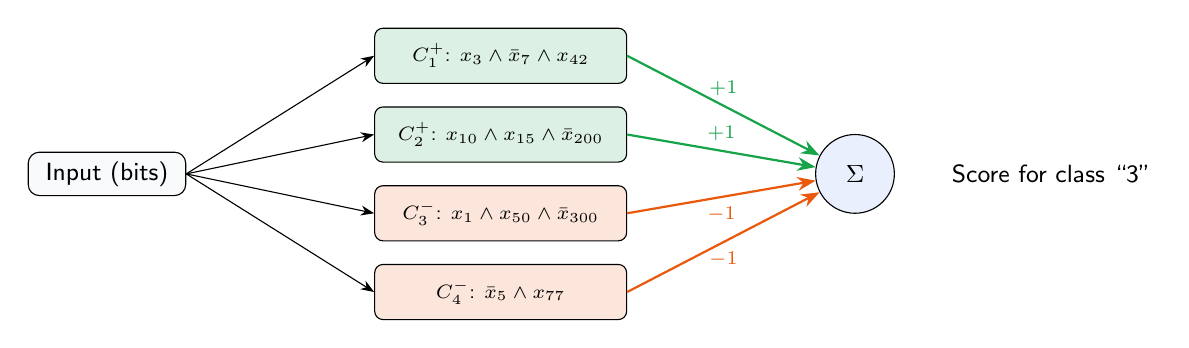
\begin{tikzpicture}[
  clause/.style={draw, rounded corners=3pt, minimum width=3.2cm,
    minimum height=0.7cm, font=\scriptsize\sffamily, align=center},
  vote/.style={-{Stealth}, thick},
  >=Stealth
]
  % Input
  \node[draw, rounded corners, fill=lightbg, minimum width=2cm,
    font=\small\sffamily] (input) at (0, 0) {Input (bits)};

  % Positive clauses
  \node[clause, fill=bitgreen!15] (c1) at (5, 1.5)
    {$C_1^+$: $x_3 \wedge \bar{x}_7 \wedge x_{42}$};
  \node[clause, fill=bitgreen!15] (c2) at (5, 0.5)
    {$C_2^+$: $x_{10} \wedge x_{15} \wedge \bar{x}_{200}$};

  % Negative clauses
  \node[clause, fill=bitorange!15] (c3) at (5, -0.5)
    {$C_3^-$: $x_1 \wedge x_{50} \wedge \bar{x}_{300}$};
  \node[clause, fill=bitorange!15] (c4) at (5, -1.5)
    {$C_4^-$: $\bar{x}_5 \wedge x_{77}$};

  % Connections
  \foreach \c in {c1,c2,c3,c4} {
    \draw[->] (input.east) -- (\c.west);
  }

  % Sum
  \node[draw, circle, minimum size=1cm, fill=bitblue!10,
    font=\small\sffamily\bfseries] (sum) at (9.5, 0) {$\Sigma$};

  \draw[vote, bitgreen] (c1.east) -- node[above, font=\scriptsize] {$+1$} (sum);
  \draw[vote, bitgreen] (c2.east) -- node[above, font=\scriptsize] {$+1$} (sum);
  \draw[vote, bitorange] (c3.east) -- node[below, font=\scriptsize] {$-1$} (sum);
  \draw[vote, bitorange] (c4.east) -- node[below, font=\scriptsize] {$-1$} (sum);

  % Output
  \node[font=\small\sffamily, right=0.6cm] at (sum.east)
    {Score for class ``3''};
\end{tikzpicture}
\caption{Tsetlin Machine clause voting. Each clause evaluates a
  conjunction of literals (an AND of selected input bits). Positive
  clauses vote for the class; negative clauses vote against. The net
  score determines the prediction.}
\label{fig:tm-voting}
\end{figure}

\subsubsection{Step 4: Learning with Tsetlin Automata}

This is where Tsetlin Machines are fundamentally different from neural
networks. There are no gradients. Instead, each literal in each clause
is controlled by a \concept{Tsetlin automaton}---a simple finite-state
machine with $2N$ states.

\begin{figure}[htbp]
\centering
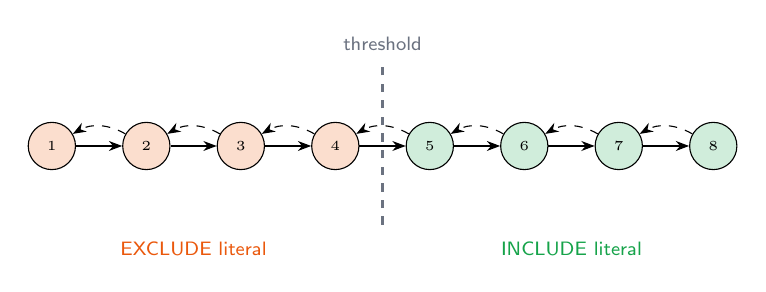
\begin{tikzpicture}[
  state/.style={draw, circle, minimum size=0.6cm, font=\tiny\sffamily,
    inner sep=0pt},
  >=Stealth
]
  % States
  \foreach \i in {1,...,4} {
    \node[state, fill=bitorange!20] (ex\i) at (\i*1.2, 0)
      {$\i$};
  }
  \foreach \i in {5,...,8} {
    \node[state, fill=bitgreen!20] (in\i) at (\i*1.2, 0)
      {$\i$};
  }

  % Arrows between states
  \foreach \i [evaluate=\i as \j using int(\i+1)] in {1,...,7} {
    \pgfmathtruncatemacro{\ii}{\i}
    \pgfmathtruncatemacro{\jj}{\j}
    \ifnum\ii<4
      \draw[->] (ex\ii) -- (ex\jj);
    \else
      \ifnum\ii=4
        \draw[->] (ex4) -- (in5);
      \else
        \draw[->] (in\ii) -- (in\jj);
      \fi
    \fi
  }
  \foreach \i [evaluate=\i as \j using int(\i-1)] in {2,...,8} {
    \pgfmathtruncatemacro{\ii}{\i}
    \pgfmathtruncatemacro{\jj}{\j}
    \ifnum\ii>5
      \draw[->, bend right=30, dashed] (in\ii) to (in\jj);
    \else
      \ifnum\ii=5
        \draw[->, bend right=30, dashed] (in5) to (ex4);
      \else
        \draw[->, bend right=30, dashed] (ex\ii) to (ex\jj);
      \fi
    \fi
  }

  % Dividing line
  \draw[thick, bitgray, dashed] (5.4, -1) -- (5.4, 1);
  \node[font=\scriptsize\sffamily, bitorange] at (3, -1.3) {EXCLUDE literal};
  \node[font=\scriptsize\sffamily, bitgreen] at (7.8, -1.3) {INCLUDE literal};

  % Labels
  \node[font=\scriptsize\sffamily, bitgray] at (5.4, 1.3) {threshold};
\end{tikzpicture}
\caption{A Tsetlin automaton with $2N = 8$ states. States 1--4 mean
  ``exclude this literal from the clause''; states 5--8 mean ``include
  it.'' Learning nudges the state left or right based on feedback.}
\label{fig:tsetlin-automaton}
\end{figure}

The learning algorithm uses stochastic feedback:

\begin{description}[leftmargin=1em]
  \item[Type~I feedback] (reward correct clauses): Reinforce included
    literals that matched the input; randomly exclude literals that
    were not helpful. This \emph{specialises} clauses.
  \item[Type~II feedback] (penalise incorrect clauses): Include
    literals that would have falsified the clause (making it output~0
    instead of erroneously voting). This \emph{corrects} clauses.
\end{description}

\begin{engineernote}
The beauty of Tsetlin automata is that they are just
\emph{counters}. Increment or decrement a state by 1 based on a
coin flip and the classification result. No floating-point
arithmetic at all. The entire training loop is integer addition,
comparison, and random number generation.
\end{engineernote}

% --- Formalisation ---
\subsection{Mathematical Summary}
\label{sec:tm-math}

Let $\bm{x} \in \{0,1\}^n$ be a binary input vector. Define the
extended literal set $L = \{x_1, \bar{x}_1, x_2, \bar{x}_2, \ldots,
x_n, \bar{x}_n\}$ with $|L| = 2n$.

Each clause $C_j$ is defined by a subset $S_j \subseteq L$ and
computes:
\begin{equation}
  C_j(\bm{x}) = \bigwedge_{\ell \in S_j} \ell
  \label{eq:tm-clause-formal}
\end{equation}

For a $K$-class problem with $m$ clauses per class (half positive,
half negative), the output for class $k$ is:
\begin{equation}
  f_k(\bm{x}) = \sum_{j=1}^{m/2} C_j^{+,k}(\bm{x})
    - \sum_{j=1}^{m/2} C_j^{-,k}(\bm{x})
  \label{eq:tm-class-score}
\end{equation}

The predicted class is $\hat{y} = \arg\max_k f_k(\bm{x})$.

The threshold parameter $T$ controls clause voting saturation (scores
are clipped to $[-T, T]$), and the specificity parameter $s$ controls
how aggressively clauses specialise during Type~I feedback.

\subsection{Performance on MNIST}
\label{sec:tm-mnist}

Tsetlin Machines achieve remarkable results on MNIST~\cite{lecun1998mnist}:

\begin{table}[htbp]
\centering
\caption{Tsetlin Machine results on MNIST. Results from the original
  TM paper~\cite{granmo2018tsetlin} and the Convolutional TM
  paper~\cite{granmo2019convtm}.}
\label{tab:tm-mnist}
\begin{tabular}{@{}lrrl@{}}
  \toprule
  \textbf{Configuration}     & \textbf{Accuracy} & \textbf{Clauses} & \textbf{Source} \\
  \midrule
  Basic TM (4{,}000/class)   & 98.2\%            & 40{,}000 & \cite{granmo2018tsetlin} \\
  Convolutional TM            & 99.3\%            & 80{,}000 & \cite{granmo2019convtm} \\
  \bottomrule
\end{tabular}
\end{table}

\subsection{Strengths and Limitations}

\begin{description}[leftmargin=1em]
  \item[Strengths:]
    No floating-point arithmetic at all (training or inference),
    fully interpretable (you can read the learned rules),
    convergence proofs exist~\cite{granmo2018tsetlin},
    naturally parallel (clauses are independent),
    robust to noise.

  \item[Limitations:]
    Requires many clauses for complex tasks (millions for high
    accuracy), limited to propositional logic (no hierarchical
    feature extraction by default), hyperparameter sensitivity
    ($T$ and $s$), less mature ecosystem than neural networks.

  \item[Open question:]
    In the standard formulation, the number of clauses and the literal
    pool are both fixed before training begins. The automata learn
    \emph{which} literals to include in each clause, but cannot create
    new clauses at runtime. Clause weighting variants can suppress
    unhelpful clauses (effectively ``turning them off''), and drop-clause
    regularisation randomly disables clauses during training (analogous
    to dropout in neural networks). However, dynamically \emph{growing}
    the clause set during training---adding clauses when the model
    detects that its current capacity is insufficient---remains an
    unexplored research direction.
\end{description}

% ============================================================================
\section{Paradigm 3: Logic Gate Networks}
\label{sec:lgn}
% ============================================================================

% --- Intuition ---
\subsection{The Idea in Plain English}

Binary Neural Networks hardcode the operation: it is always XNOR.
Tsetlin Machines hardcode the operation: it is always AND (within
clauses). But what if the network could \emph{choose} which logic
gate to use at each connection?

A Logic Gate Network~\cite{petersen2022difflogic} is a layered network where each ``neuron'' is
a 2-input logic gate, and both the gate's \emph{inputs} (which two
signals to connect) and its \emph{type} (AND, OR, XOR, NAND, etc.)
are learned during training.

\begin{analogy}
Imagine building a circuit on a breadboard. You have a box of
different logic gate chips (AND, OR, XOR, NAND, NOR, XNOR). A
Logic Gate Network is like having a robot that tries different chips
in each socket and different wiring configurations, testing each
combination, and gradually settling on the circuit that best solves
the classification problem.
\end{analogy}

% --- Mechanism ---
\subsection{How It Works}

\subsubsection{The 16 Possible 2-Input Gates}

Two binary inputs can produce $2^{2^2} = 16$ possible logic functions.
These include the familiar gates plus some degenerate cases:

\begin{figure}[htbp]
\centering
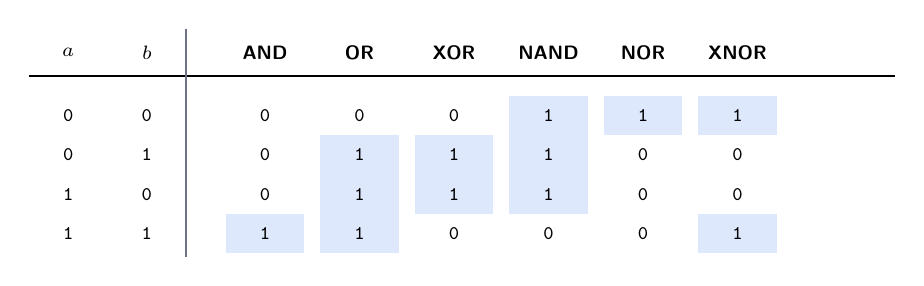
\begin{tikzpicture}[
  cell/.style={minimum width=1.0cm, minimum height=0.5cm,
    font=\scriptsize\ttfamily, inner sep=0pt},
  header/.style={cell, font=\scriptsize\sffamily\bfseries},
  >=Stealth
]
  % Table header
  \node[header] at (0, 0.8) {$a$};
  \node[header] at (1, 0.8) {$b$};
  \draw[thick] (-0.5, 0.5) -- (10.5, 0.5);

  % Input rows
  \foreach \a/\b/\row in {0/0/0, 0/1/-0.5, 1/0/-1, 1/1/-1.5} {
    \node[cell] at (0, \row) {\a};
    \node[cell] at (1, \row) {\b};
  }

  % Selected gates - explicit nodes to avoid nested foreach issues
  % AND
  \node[header] at (2.5, 0.8) {AND};
  \node[cell] at (2.5, 0) {0}; \node[cell] at (2.5, -0.5) {0};
  \node[cell] at (2.5, -1) {0}; \node[cell, fill=bitblue!15] at (2.5, -1.5) {1};
  % OR
  \node[header] at (3.7, 0.8) {OR};
  \node[cell] at (3.7, 0) {0}; \node[cell, fill=bitblue!15] at (3.7, -0.5) {1};
  \node[cell, fill=bitblue!15] at (3.7, -1) {1}; \node[cell, fill=bitblue!15] at (3.7, -1.5) {1};
  % XOR
  \node[header] at (4.9, 0.8) {XOR};
  \node[cell] at (4.9, 0) {0}; \node[cell, fill=bitblue!15] at (4.9, -0.5) {1};
  \node[cell, fill=bitblue!15] at (4.9, -1) {1}; \node[cell] at (4.9, -1.5) {0};
  % NAND
  \node[header] at (6.1, 0.8) {NAND};
  \node[cell, fill=bitblue!15] at (6.1, 0) {1}; \node[cell, fill=bitblue!15] at (6.1, -0.5) {1};
  \node[cell, fill=bitblue!15] at (6.1, -1) {1}; \node[cell] at (6.1, -1.5) {0};
  % NOR
  \node[header] at (7.3, 0.8) {NOR};
  \node[cell, fill=bitblue!15] at (7.3, 0) {1}; \node[cell] at (7.3, -0.5) {0};
  \node[cell] at (7.3, -1) {0}; \node[cell] at (7.3, -1.5) {0};
  % XNOR
  \node[header] at (8.5, 0.8) {XNOR};
  \node[cell, fill=bitblue!15] at (8.5, 0) {1}; \node[cell] at (8.5, -0.5) {0};
  \node[cell] at (8.5, -1) {0}; \node[cell, fill=bitblue!15] at (8.5, -1.5) {1};

  % Separator
  \draw[bitgray, thick] (1.5, 1.1) -- (1.5, -1.8);
\end{tikzpicture}
\caption{Truth tables for six commonly used 2-input gates. There are 16
  possible functions in total. An LGN learns which function each node
  should implement.}
\label{fig:truth-tables}
\end{figure}

\subsubsection{Differentiable Gate Selection}

The core trick of LGNs is making the discrete choice of gate type
\emph{differentiable} so that gradient descent can be used for
training.

Each node maintains a probability distribution over the 16 possible
gate functions. During training, the output is a weighted average:

\begin{equation}
  \text{output} = \sum_{g=0}^{15} p_g \cdot f_g(a, b)
  \label{eq:lgn-soft}
\end{equation}

where $p_g$ is the (learnable) probability of gate $g$ and $f_g(a,b)$
is gate $g$'s output for inputs $a, b$.

\begin{figure}[htbp]
\centering
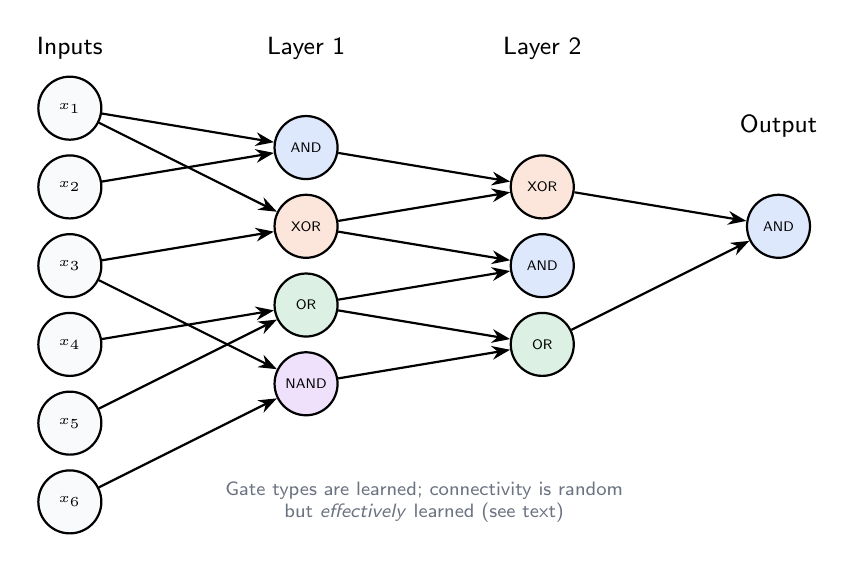
\begin{tikzpicture}[
  node/.style={draw, circle, minimum size=0.8cm, font=\tiny\sffamily,
    inner sep=0pt, line width=0.8pt},
  >=Stealth
]
  % Input layer
  \foreach \i in {1,...,6} {
    \node[node, fill=lightbg] (in\i) at (0, 5.5-\i) {$x_\i$};
  }

  % Hidden layer 1
  \foreach \i/\gate/\col in {1/AND/bitblue, 2/XOR/bitorange,
    3/OR/bitgreen, 4/NAND/bitpurple} {
    \node[node, fill=\col!15] (h1\i) at (3, 5-\i) {\gate};
  }

  % Hidden layer 2
  \foreach \i/\gate/\col in {1/XOR/bitorange, 2/AND/bitblue,
    3/OR/bitgreen} {
    \node[node, fill=\col!15] (h2\i) at (6, 4.5-\i) {\gate};
  }

  % Output
  \node[node, fill=bitblue!15] (out) at (9, 3) {AND};

  % Connections (selected, not all-to-all)
  \draw[->, thick] (in1) -- (h11);
  \draw[->, thick] (in2) -- (h11);
  \draw[->, thick] (in1) -- (h12);
  \draw[->, thick] (in3) -- (h12);
  \draw[->, thick] (in4) -- (h13);
  \draw[->, thick] (in5) -- (h13);
  \draw[->, thick] (in3) -- (h14);
  \draw[->, thick] (in6) -- (h14);

  \draw[->, thick] (h11) -- (h21);
  \draw[->, thick] (h12) -- (h21);
  \draw[->, thick] (h12) -- (h22);
  \draw[->, thick] (h13) -- (h22);
  \draw[->, thick] (h13) -- (h23);
  \draw[->, thick] (h14) -- (h23);

  \draw[->, thick] (h21) -- (out);
  \draw[->, thick] (h23) -- (out);

  % Labels
  \node[font=\small\sffamily, above] at (0, 5) {Inputs};
  \node[font=\small\sffamily, above] at (3, 5) {Layer 1};
  \node[font=\small\sffamily, above] at (6, 5) {Layer 2};
  \node[font=\small\sffamily, above] at (9, 4) {Output};

  % Annotation
  \node[font=\scriptsize\sffamily, bitgray, align=center] at (4.5, -0.5)
    {Gate types are learned; connectivity is random\\but \emph{effectively}
    learned (see text)};
\end{tikzpicture}
\caption{A Logic Gate Network. Each node is a 2-input logic gate whose
  type is learned through differentiable relaxation. The connectivity
  is initially random but effectively learned through gate-type
  selection (see below). At inference time, this is a pure logic
  circuit with zero arithmetic.}
\label{fig:lgn-architecture}
\end{figure}

\subsubsection{How Connectivity Is ``Learned''}
\label{sec:lgn-connectivity}

The equations in the next subsection show how gate \emph{types} are
learned, but how does the network learn its \emph{wiring}---which two
signals feed into each gate?

In the original DiffLogic architecture~\cite{petersen2022difflogic},
the answer is surprisingly indirect: \textbf{connections are assigned
randomly and remain fixed.} Each gate is randomly wired to two outputs
from the previous layer at initialisation and never rewired.

This sounds limiting, but it works because of a key observation:
among the 16 possible 2-input Boolean functions, six of them
\emph{effectively ignore one or both inputs}:

\begin{table}[htbp]
\centering
\caption{Of the 16 possible 2-input Boolean functions, six ignore
  at least one input. By learning to become one of these functions,
  a gate can effectively ``disconnect'' an unwanted input.}
\label{tab:gate-disconnect}
\begin{tabular}{@{}llll@{}}
  \toprule
  \textbf{Gate function} & \textbf{Output} & \textbf{Ignores}
    & \textbf{Effect} \\
  \midrule
  Constant 0  & always 0             & both $a$ and $b$
    & dead gate (pruned) \\
  Constant 1  & always 1             & both $a$ and $b$
    & dead gate (pruned) \\
  Pass-through $a$  & $a$            & input $b$
    & wire from $a$ only \\
  Pass-through $b$  & $b$            & input $a$
    & wire from $b$ only \\
  NOT $a$     & $\overline{a}$       & input $b$
    & inverter on $a$ \\
  NOT $b$     & $\overline{b}$       & input $a$
    & inverter on $b$ \\
  \bottomrule
\end{tabular}
\end{table}

\begin{keyinsight}
Connectivity learning is \emph{subsumed by gate-type learning.} When
the training process selects a gate type, it simultaneously decides
the effective wiring:
\begin{itemize}[leftmargin=1em]
  \item A gate that learns ``AND'' uses both inputs.
  \item A gate that learns ``pass-through $a$'' effectively
    disconnects input $b$, acting as a simple wire.
  \item A gate that learns ``constant 0'' effectively disconnects
    from the network entirely.
\end{itemize}
The network is deliberately \emph{over-provisioned}---it starts with
many more gates than needed, and training prunes unnecessary
connections by turning gates into pass-throughs or constants.
This is why the single softmax-over-16-gates mechanism
(\cref{eq:lgn-soft}) is sufficient to learn both gate types
\emph{and} effective connectivity.
\end{keyinsight}

\subsubsection{Training: From Soft to Hard}

During training, the network operates in ``soft'' mode: gate outputs
are real-valued probabilities, and gradients flow through the weighted
sum. As training progresses, the distributions sharpen until each node
has a clear winner. Two common techniques drive this sharpening:
\emph{temperature annealing} gradually lowers a temperature parameter
that controls how peaked the softmax distribution is---high temperature
gives near-uniform probabilities, low temperature approaches a hard
one-hot selection. The \emph{Gumbel-softmax} trick adds carefully
calibrated random noise before the softmax, which lets the network
explore different gate choices early in training while still permitting
gradient flow (unlike a hard \texttt{argmax}, which is not
differentiable).

At inference time, each node commits to its most probable gate type
and operates in pure binary logic---no floating-point, no
probabilities.

\begin{figure}[htbp]
\centering
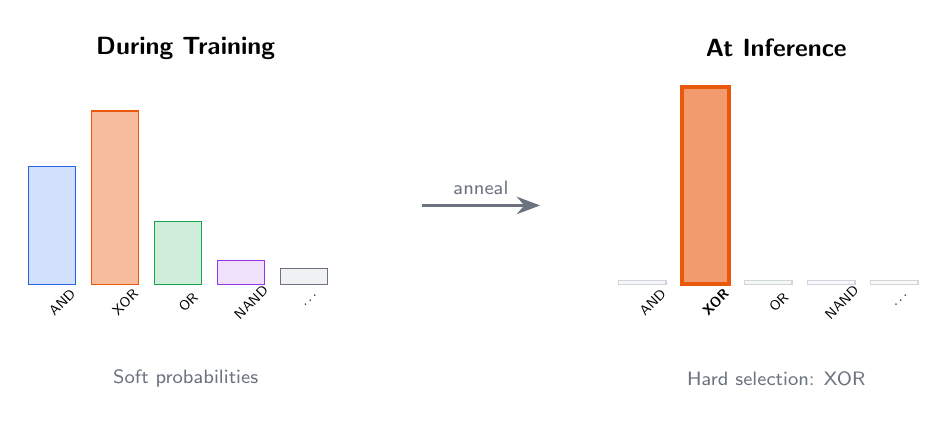
\begin{tikzpicture}[>=Stealth]
  % Training phase
  \begin{scope}
    \node[font=\small\sffamily\bfseries] at (2, 3) {During Training};
    \draw[fill=bitblue!20, draw=bitblue] (0, 0) rectangle (0.6, 1.5);
    \draw[fill=bitorange!40, draw=bitorange] (0.8, 0) rectangle (1.4, 2.2);
    \draw[fill=bitgreen!20, draw=bitgreen] (1.6, 0) rectangle (2.2, 0.8);
    \draw[fill=bitpurple!15, draw=bitpurple] (2.4, 0) rectangle (3.0, 0.3);
    \draw[fill=bitgray!10, draw=bitgray] (3.2, 0) rectangle (3.8, 0.2);
    \node[font=\tiny\sffamily, below, rotate=45] at (0.3, -0.1) {AND};
    \node[font=\tiny\sffamily, below, rotate=45] at (1.1, -0.1) {XOR};
    \node[font=\tiny\sffamily, below, rotate=45] at (1.9, -0.1) {OR};
    \node[font=\tiny\sffamily, below, rotate=45] at (2.7, -0.1) {NAND};
    \node[font=\tiny\sffamily, below, rotate=45] at (3.5, -0.1) {\ldots};
    \node[font=\scriptsize\sffamily, bitgray] at (2, -1.2)
      {Soft probabilities};
  \end{scope}

  % Arrow
  \draw[->, very thick, bitgray] (5, 1) -- (6.5, 1)
    node[midway, above, font=\scriptsize\sffamily] {anneal};

  % Inference phase
  \begin{scope}[xshift=7.5cm]
    \node[font=\small\sffamily\bfseries] at (2, 3) {At Inference};
    \draw[fill=bitblue!5, draw=bitgray!30] (0, 0) rectangle (0.6, 0.05);
    \draw[fill=bitorange!60, draw=bitorange, line width=1.5pt]
      (0.8, 0) rectangle (1.4, 2.5);
    \draw[fill=bitgreen!5, draw=bitgray!30] (1.6, 0) rectangle (2.2, 0.05);
    \draw[fill=bitpurple!5, draw=bitgray!30] (2.4, 0) rectangle (3.0, 0.05);
    \draw[fill=bitgray!5, draw=bitgray!30] (3.2, 0) rectangle (3.8, 0.05);
    \node[font=\tiny\sffamily, below, rotate=45] at (0.3, -0.1) {AND};
    \node[font=\tiny\sffamily\bfseries, below, rotate=45] at (1.1, -0.1) {XOR};
    \node[font=\tiny\sffamily, below, rotate=45] at (1.9, -0.1) {OR};
    \node[font=\tiny\sffamily, below, rotate=45] at (2.7, -0.1) {NAND};
    \node[font=\tiny\sffamily, below, rotate=45] at (3.5, -0.1) {\ldots};
    \node[font=\scriptsize\sffamily, bitgray] at (2, -1.2)
      {Hard selection: XOR};
  \end{scope}
\end{tikzpicture}
\caption{Gate selection during training (soft, differentiable
  probabilities) versus inference (hard, discrete gate commitment).
  Temperature annealing gradually sharpens the distribution.}
\label{fig:lgn-annealing}
\end{figure}

% --- Formalisation ---
\subsection{Mathematical Summary}
\label{sec:lgn-math}

Let each node $i$ in layer $\ell$ receive two binary inputs
$a_i^{(\ell)}, b_i^{(\ell)} \in \{0, 1\}$ from the previous layer.

The node maintains a logit vector $\bm{\alpha}_i \in \mathbb{R}^{16}$,
converted to probabilities via softmax with temperature $\tau$:
\begin{equation}
  p_g^{(i)} = \frac{\exp(\alpha_g^{(i)} / \tau)}
    {\sum_{g'=0}^{15} \exp(\alpha_{g'}^{(i)} / \tau)}
  \label{eq:lgn-softmax}
\end{equation}

The soft output during training is:
\begin{equation}
  o_i^{(\ell)} = \sum_{g=0}^{15} p_g^{(i)} \cdot
    \operatorname{TruthTable}(g, a_i^{(\ell)}, b_i^{(\ell)})
  \label{eq:lgn-soft-output}
\end{equation}

where $\operatorname{TruthTable}(g, a, b) \in \{0, 1\}$ is the output
of the $g$-th Boolean function for inputs $(a, b)$.

At inference ($\tau \to 0$):
\begin{equation}
  o_i^{(\ell)} = \operatorname{TruthTable}\!\left(
    \arg\max_g \alpha_g^{(i)},\; a_i^{(\ell)},\; b_i^{(\ell)}\right)
  \label{eq:lgn-hard-output}
\end{equation}

\subsection{Performance and Scale}

LGNs are relatively new. Published results include:

\begin{table}[htbp]
\centering
\caption{Logic Gate Network results on MNIST. Connection optimisation
  substantially changes the gate-count picture, but the newest result is a
  preprint and needs independent replication~\cite{petersen2022difflogic,mommen2026fullytrainable}.}
\label{tab:lgn-perf}
\begin{tabular}{@{}lrrl@{}}
  \toprule
  \textbf{Network} & \textbf{MNIST} & \textbf{Gates} & \textbf{Note} \\
  \midrule
  DiffLogic (small)~\cite{petersen2022difflogic} & 97.7\% & 48k  & 6 layers, 8k gates/layer \\
  DiffLogic~\cite{petersen2022difflogic}          & 98.5\% & 384k & 6 layers, 64k gates/layer \\
  Connection-optimised LGN~\cite{mommen2026fullytrainable} & 98.92\% & 16k & 2 layers, 8k gates/layer \\
  \bottomrule
\end{tabular}
\end{table}

Recent work changes two important limitations of the original LGN
formulation. A reparameterisation reduces binary-input model size by
$4\times$, accelerates the backward pass, and reports stable CIFAR-100
accuracy~\cite{ruttgers2025light}. Separately, learning the connections as
well as the gate types reports 98.92\% MNIST accuracy with two layers of
8{,}000 gates---almost $50\times$ fewer gates than a comparable
fixed-connection construction~\cite{mommen2026fullytrainable}. These
results make sparse, learned Boolean composition a stronger CPU research
lead, but they do not yet establish transformer-scale circuits.

\subsection{Strengths and Limitations}

\begin{description}[leftmargin=1em]
  \item[Strengths:]
    Pure logic at inference, learned gate type and connectivity, and a
    plausible path to sparse, branch-light CPU evaluation when gate outputs
    are stored and traversed in contiguous packed arrays.

  \item[Limitations:]
    2-input restriction can require deep networks; training is slower than
    standard backpropagation (16-way softmax per node); and a gate graph
    with irregular fan-out can lose to a small SIMD integer MLP on CPU
    despite performing no multiplications.
\end{description}

% ============================================================================
\section{Paradigm 4: Kolmogorov-Arnold Networks and LUT Compilation}
\label{sec:kan}
% ============================================================================

% --- Intuition ---
\subsection{The Idea in Plain English}

The three paradigms we have seen so far all simplify the neuron: strip
it down to binary operations and accept some accuracy loss. This
fourth paradigm does the opposite during training: it makes each
connection \emph{more} complex than a traditional weight. Then, once
training is done, it compiles that complexity into a simple lookup
table.

\begin{analogy}
Imagine learning to cook a complex sauce. At first, you follow an
elaborate recipe (training): you measure precisely, taste repeatedly,
adjust seasoning. Once you have perfected it, you write down just
the final quantities on an index card (lookup table). Now you can
recreate the sauce by just reading the card---no skill required,
just follow the numbers. The complexity happened once; the
deployment is trivial.
\end{analogy}

The ``elaborate recipe'' is a \concept{Kolmogorov-Arnold Network}
(KAN)~\cite{liu2024kan}, where every connection is a learnable curve (B-spline). The
``index card'' is a \concept{lookup table} (LUT), where the curve is
sampled at fixed points and stored in memory.

% --- Mechanism ---
\subsection{The Kolmogorov-Arnold Theorem}

KANs are grounded in a mathematical theorem from 1957~\cite{kolmogorov1957}. In plain
terms:

\begin{keyinsight}[title={Kolmogorov-Arnold Representation Theorem~\cite{kolmogorov1957}}]
\emph{Any} continuous function of multiple variables can be written as
a composition of continuous functions of \emph{one} variable and
addition. You never need multiplication of two variables---just
clever single-variable functions and sums.
\end{keyinsight}

Formally, for any continuous function $f : [0,1]^n \to \mathbb{R}$:
\begin{equation}
  f(x_1, \ldots, x_n) = \sum_{q=0}^{2n}
    \Phi_q\!\left(\sum_{p=1}^{n} \phi_{q,p}(x_p)\right)
  \label{eq:ka-theorem}
\end{equation}

where $\phi_{q,p}$ and $\Phi_q$ are continuous single-variable
functions. The theorem says these functions exist but does not tell
us what they look like---the network learns them.

\subsection{How a KAN Layer Works}

\subsubsection{Traditional MLP: Fixed Activations, Learnable Weights}

Recall that in a standard MLP, each connection has a single number
(weight), and the activation function is the same for all neurons in
a layer:

\begin{equation}
  \text{MLP layer: } \bm{y} = \sigma(\bm{W}\bm{x} + \bm{b})
  \label{eq:mlp-layer}
\end{equation}

\subsubsection{KAN: Learnable Activations, No Weights}

A KAN~\cite{liu2024kan} \emph{replaces} the weight-then-activate pattern. Each edge has
its own learnable function $\phi_{i,j}$. Nodes just sum:

\begin{equation}
  \text{KAN layer: } y_i = \sum_{j=1}^{n} \phi_{i,j}(x_j)
  \label{eq:kan-layer}
\end{equation}

\begin{figure}[htbp]
\centering
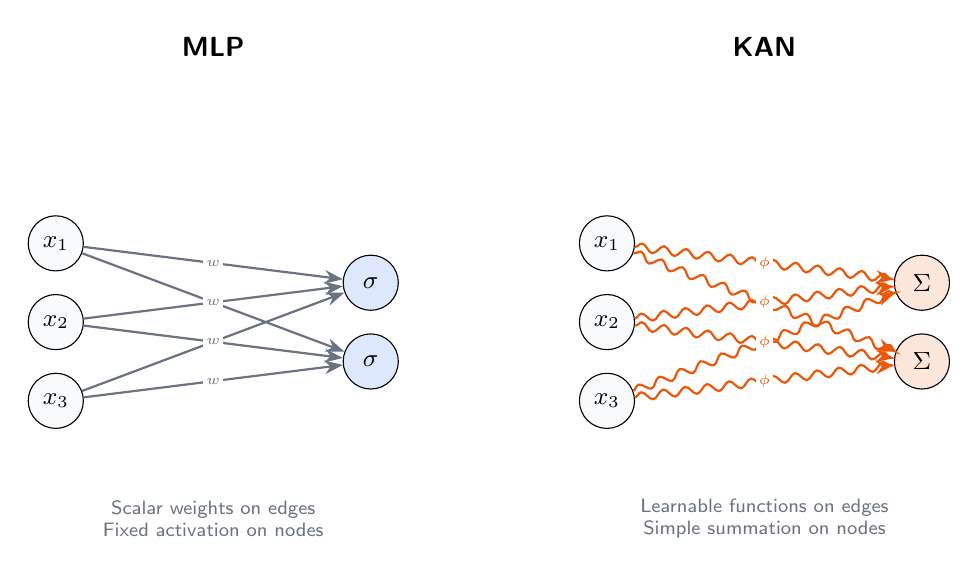
\begin{tikzpicture}[
  node/.style={draw, circle, minimum size=0.7cm, font=\small, inner sep=0pt},
  >=Stealth
]
  % --- MLP side ---
  \node[font=\sffamily\bfseries] at (2, 4.5) {MLP};

  % Input
  \foreach \i in {1,2,3} {
    \node[node, fill=lightbg] (mi\i) at (0, 3-\i) {$x_\i$};
  }
  % Output
  \foreach \i in {1,2} {
    \node[node, fill=bitblue!15] (mo\i) at (4, 2.5-\i) {$\sigma$};
  }
  % Connections (straight lines = scalar weights)
  \foreach \i in {1,2,3} {
    \foreach \j in {1,2} {
      \draw[->, thick, bitgray] (mi\i) -- (mo\j)
        node[midway, font=\tiny, fill=white, inner sep=1pt] {$w$};
    }
  }

  % --- KAN side ---
  \node[font=\sffamily\bfseries] at (9, 4.5) {KAN};

  % Input
  \foreach \i in {1,2,3} {
    \node[node, fill=lightbg] (ki\i) at (7, 3-\i) {$x_\i$};
  }
  % Output
  \foreach \i in {1,2} {
    \node[node, fill=bitorange!15] (ko\i) at (11, 2.5-\i) {$\Sigma$};
  }
  % Connections (wavy lines = learnable functions)
  \foreach \i in {1,2,3} {
    \foreach \j in {1,2} {
      \draw[->, thick, bitorange, decorate,
        decoration={snake, amplitude=1.5pt, segment length=8pt}]
        (ki\i) -- (ko\j)
        node[midway, font=\tiny, fill=white, inner sep=1pt] {$\phi$};
    }
  }

  % Labels
  \node[font=\scriptsize\sffamily, bitgray, align=center] at (2, -1.5)
    {Scalar weights on edges\\Fixed activation on nodes};
  \node[font=\scriptsize\sffamily, bitgray, align=center] at (9, -1.5)
    {Learnable functions on edges\\Simple summation on nodes};
\end{tikzpicture}
\caption{MLP vs KAN architecture. In an MLP (left), edges carry scalar
  weights and nodes apply a fixed activation. In a KAN (right), edges
  carry learnable functions (B-splines) and nodes simply sum. The wavy
  lines represent that each connection is an entire curve, not a single
  number.}
\label{fig:mlp-vs-kan}
\end{figure}

\subsubsection{B-Spline Functions}

Each edge function $\phi_{i,j}$ is parameterised as a B-spline with
$G$ grid points and order $k$ (typically $k=3$, cubic). The function
is:
\begin{equation}
  \phi_{i,j}(x) = w_b \cdot \operatorname{SiLU}(x)
    + w_s \cdot \sum_{m=0}^{G+k} c_m \cdot B_m^k(x)
  \label{eq:kan-spline}
\end{equation}

where $B_m^k$ are B-spline basis functions, $c_m$ are learnable
coefficients, and $w_b, w_s$ are scaling factors.

\begin{engineernote}
A B-spline is just a smooth, piecewise polynomial curve controlled
by a set of ``control points'' (the coefficients $c_m$). If you have
used Bézier curves in graphics, B-splines are their generalisation.
The grid determines where the curve's ``knots'' are---points where
one polynomial piece ends and the next begins.
\end{engineernote}

\begin{figure}[htbp]
\centering
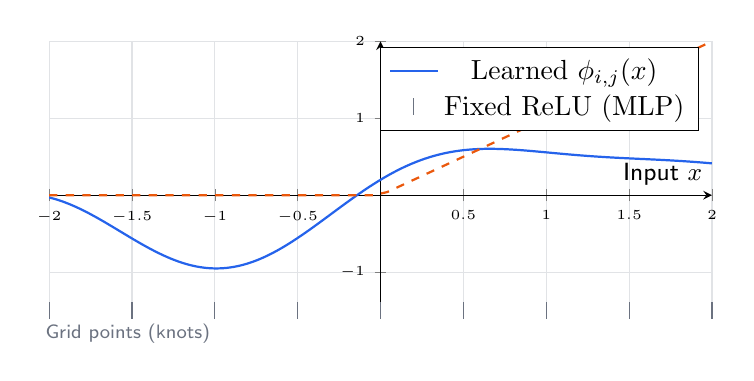
\begin{tikzpicture}
  \begin{axis}[
    width=10cm, height=5cm,
    xlabel={Input $x$}, ylabel={$\phi(x)$},
    grid=major, grid style={bitgray!20},
    xmin=-2, xmax=2, ymin=-1.5, ymax=2,
    axis lines=middle,
    every axis label/.style={font=\small\sffamily},
    tick label style={font=\tiny}
  ]
    % A sample spline-like function
    \addplot[thick, bitblue, smooth, domain=-2:2, samples=100]
      {0.3*x + 0.5*sin(deg(2*x)) + 0.2*cos(deg(3*x))};
    \addlegendentry{Learned $\phi_{i,j}(x)$}

    % Grid points
    \foreach \gp in {-2, -1.5, -1, -0.5, 0, 0.5, 1, 1.5, 2} {
      \addplot[only marks, mark=|, mark size=3pt, bitgray]
        coordinates {(\gp, -1.5)};
    }

    % ReLU for comparison
    \addplot[thick, bitorange, dashed, domain=-2:2, samples=50]
      {max(0, x)};
    \addlegendentry{Fixed ReLU (MLP)}
  \end{axis}

  % Grid label
  \node[font=\scriptsize\sffamily, bitgray] at (1, -0.3)
    {Grid points (knots)};
\end{tikzpicture}
\caption{A learnable B-spline activation (blue) vs.\ a fixed ReLU
  (orange dashed). The B-spline can learn arbitrary shapes, capturing
  complex input--output relationships that a ReLU cannot. The grid
  points (tick marks at bottom) define the spline's resolution.}
\label{fig:kan-spline}
\end{figure}

% --- LUT Compilation ---
\subsection{From Splines to Lookup Tables}
\label{sec:lut-compilation}

Here is where the computation-memory trade-off becomes concrete. After
training, each spline function $\phi_{i,j}(x)$ is a fixed curve. We
can \emph{compile} it:

\begin{enumerate}[leftmargin=2em]
  \item \textbf{Sample} the spline at $L$ evenly spaced points.
  \item \textbf{Quantise} the output values to a fixed-point format
    (e.g., int8).
  \item \textbf{Store} the $L$ values in an array---the lookup table.
  \item At inference, \textbf{look up} the nearest entry (or
    interpolate between two adjacent entries).
\end{enumerate}

\begin{figure}[htbp]
\centering
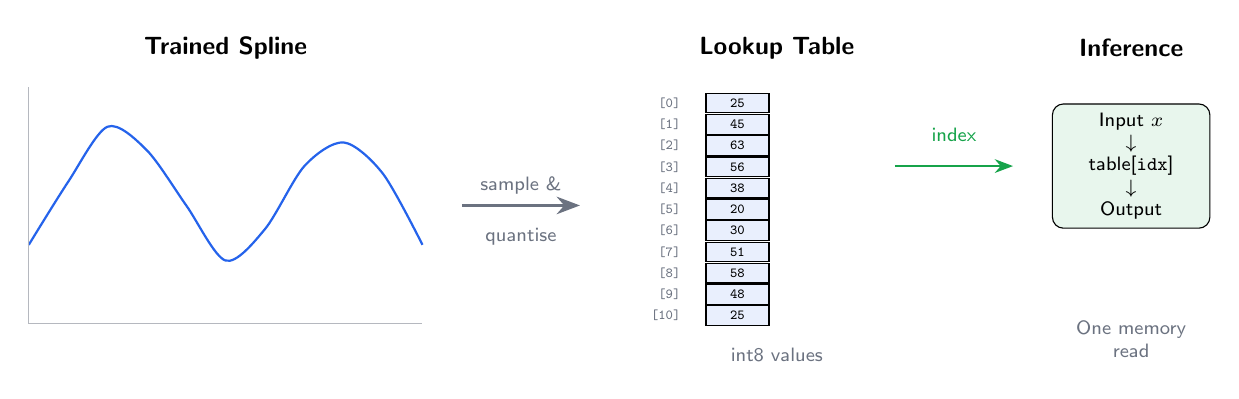
\begin{tikzpicture}[>=Stealth]
  % Spline
  \begin{scope}
    \node[font=\small\sffamily\bfseries] at (2.5, 3.5) {Trained Spline};
    \draw[thick, bitblue, smooth] plot coordinates
      {(0,1) (0.5,1.8) (1,2.5) (1.5,2.2) (2,1.5) (2.5,0.8)
       (3,1.2) (3.5,2.0) (4,2.3) (4.5,1.9) (5,1.0)};
    \draw[bitgray!50] (0, 0) -- (5, 0);
    \draw[bitgray!50] (0, 0) -- (0, 3);
  \end{scope}

  % Arrow
  \draw[->, very thick, bitgray] (5.5, 1.5) -- (7, 1.5)
    node[midway, above, font=\scriptsize\sffamily] {sample \&};
  \node[font=\scriptsize\sffamily, bitgray] at (6.25, 1.1) {quantise};

  % LUT
  \begin{scope}[xshift=7.5cm]
    \node[font=\small\sffamily\bfseries] at (2, 3.5) {Lookup Table};
    \foreach \i/\v/\q in {0/1.0/25, 1/1.8/45, 2/2.5/63,
      3/2.2/56, 4/1.5/38, 5/0.8/20, 6/1.2/30, 7/2.0/51,
      8/2.3/58, 9/1.9/48, 10/1.0/25} {
      \pgfmathsetmacro{\ypos}{2.8 - \i * 0.27}
      \node[draw, minimum width=0.8cm, minimum height=0.25cm,
        font=\tiny\ttfamily, fill=bitblue!10, inner sep=0pt]
        at (1.5, \ypos) {\q};
      \node[font=\tiny\ttfamily, bitgray, left] at (0.9, \ypos) {[\i]};
    }
    \node[font=\scriptsize\sffamily, bitgray] at (2, -0.4)
      {int8 values};
  \end{scope}

  % Usage arrow
  \draw[->, thick, bitgreen] (11, 2) -- (12.5, 2);
  \node[font=\scriptsize\sffamily, bitgreen] at (11.75, 2.4) {index};

  % Inference
  \begin{scope}[xshift=13cm]
    \node[font=\small\sffamily\bfseries] at (1, 3.5) {Inference};
    \node[draw, rounded corners, fill=bitgreen!10,
      font=\scriptsize\sffamily, align=center, minimum width=2cm]
      at (1, 2) {Input $x$\\$\downarrow$\\table[\texttt{idx}]\\$\downarrow$\\Output};
    \node[font=\scriptsize\sffamily, bitgray, align=center] at (1, -0.2)
      {One memory\\read};
  \end{scope}
\end{tikzpicture}
\caption{LUT compilation: a trained B-spline (left) is sampled at
  regular intervals and quantised to int8 values (centre). At
  inference, evaluating the function becomes a single array index
  operation (right)---no arithmetic needed.}
\label{fig:lut-compilation}
\end{figure}

\begin{keyinsight}
After LUT compilation, the entire ``activation function'' is a single
memory read. The spline's mathematical complexity exists only during
training. At deployment, every edge in the network costs exactly one
table lookup---a cost comparable to a single bitwise operation on
most hardware.
\end{keyinsight}

% --- ULEEN ---
\subsection{ULEEN: The Extreme Case}
\label{sec:uleen}

The \concept{Ultra-Low-Energy Edge Neural Network}
(ULEEN)~\cite{uleen2023} takes the LUT idea to its logical extreme:
the entire network is just tables. No splines, no arithmetic, not even
during training. The input features are grouped, each group indexes
into a table, and the outputs are summed.

\begin{table}[htbp]
\centering
\caption{ULEEN results on MNIST.}
\label{tab:uleen}
\begin{tabular}{@{}lr@{}}
  \toprule
  \textbf{Metric} & \textbf{Value} \\
  \midrule
  Accuracy          & 96.2\% \\
  Model size         & 16.9\,kB \\
  Inference latency  & 0.21\,$\mu$s \\
  Throughput         & 14.3\,M inferences/s \\
  \bottomrule
\end{tabular}
\end{table}

% --- Formalisation ---
\subsection{Mathematical Summary}
\label{sec:kan-math}

A KAN layer $\Phi$ mapping $\mathbb{R}^{n_\text{in}}$ to
$\mathbb{R}^{n_\text{out}}$ is defined by a matrix of univariate
functions:
\begin{equation}
  \Phi = \{\phi_{i,j}\}_{1 \leq i \leq n_\text{out},\;
    1 \leq j \leq n_\text{in}}
  \label{eq:kan-matrix}
\end{equation}

The layer computation is:
\begin{equation}
  y_i = \sum_{j=1}^{n_\text{in}} \phi_{i,j}(x_j),
  \quad i = 1, \ldots, n_\text{out}
  \label{eq:kan-layer-formal}
\end{equation}

Each function has $G + k + 2$ learnable parameters (B-spline
coefficients plus scaling), compared to 1 parameter per edge in an MLP.
A KAN layer with width $n$ and grid size $G$ has $O(n^2 (G+k))$
parameters vs.\ $O(n^2)$ for an MLP layer.

After LUT compilation with $L$ samples per function, each
$\phi_{i,j}$ is replaced by:
\begin{equation}
  \hat{\phi}_{i,j}(x) = \operatorname{table}_{i,j}
    \!\left[\operatorname{round}\!\left(\frac{x - x_{\min}}
    {x_{\max} - x_{\min}} \cdot (L-1)\right)\right]
  \label{eq:lut-eval}
\end{equation}

This is an $O(1)$ memory access, reducing inference to
$n_\text{in} \times n_\text{out}$ table lookups plus
$n_\text{out}$ integer additions per layer.

\subsection{Strengths and Limitations}

\begin{description}[leftmargin=1em]
  \item[Strengths:]
    Theoretically grounded (Kolmogorov-Arnold theorem~\cite{kolmogorov1957}), highest
    accuracy among bitwise-deployable approaches, LUT compilation
    enables zero-arithmetic inference, naturally maps to FPGA LUT
    fabric~\cite{polylut2023, lutkan2025}, graceful accuracy-memory trade-off (more table entries
    = more accuracy).

  \item[Limitations:]
    Training is slow ($\sim$10$\times$ slower than MLP with same
    parameter count), requires floating-point during training,
    LUT size grows with input precision and grid resolution,
    relatively new (2024--2025) with evolving best practices.
\end{description}

% ============================================================================
\section{Comparing the Four Paradigms}
\label{sec:comparison}
% ============================================================================

With all four paradigms introduced, we can now compare them
systematically. \Cref{tab:paradigm-comparison} provides a side-by-side
summary, and the radar chart in \cref{fig:radar} visualises the
trade-offs.

\begin{table}[htbp]
\centering
\caption{Side-by-side comparison of the four bitwise AI paradigms
  on key engineering criteria~\cite{courbariaux2016bnn, granmo2018tsetlin, petersen2022difflogic, liu2024kan}. Ratings: \textbf{H}igh, \textbf{M}edium,
  \textbf{L}ow.}
\label{tab:paradigm-comparison}
\small
\begin{tabular}{@{}p{2.8cm}cccc@{}}
  \toprule
  \textbf{Criterion} & \textbf{BNN} & \textbf{Tsetlin} &
    \textbf{LGN} & \textbf{KAN/LUT} \\
  \midrule
  MNIST accuracy & 98.6\% & 99.4\% & 98.1\% & 98.0\% \\
  Inference ops & XNOR+pop & AND+count & gate eval & LUT read \\
  Training method & STE+backprop & Automata & Backprop & Backprop \\
  Needs FP at train? & Yes & No & Yes & Yes \\
  Needs FP at inference? & BatchNorm & No & No & No \\
  Model size & Very small & Medium & Small & Configurable \\
  Interpretability & Low & High & Medium & Low \\
  Hardware mapping & Good & Good & Excellent & Excellent \\
  Maturity & High & Medium & Low & Low \\
  \bottomrule
\end{tabular}
\end{table}

\begin{figure}[htbp]
\centering
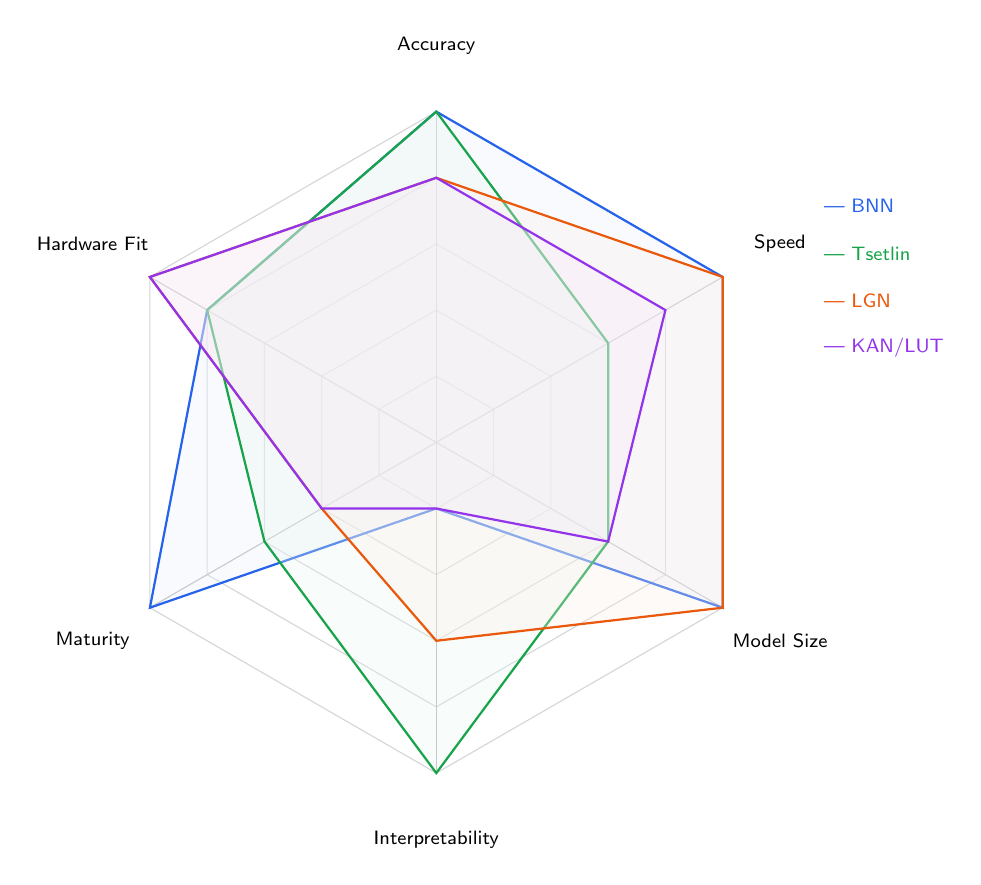
\begin{tikzpicture}[scale=1.2]
  % Axis angles: 90, 30, -30, -90, -150, 150
  % Grid pentagons
  \foreach \level in {1,2,3,4,5} {
    \draw[bitgray!30]
      (90:\level*0.7) -- (30:\level*0.7) -- (-30:\level*0.7) --
      (-90:\level*0.7) -- (-150:\level*0.7) -- (150:\level*0.7) -- cycle;
  }

  % Axes
  \foreach \angle in {90, 30, -30, -90, -150, 150} {
    \draw[bitgray!50] (0,0) -- (\angle:3.5);
  }

  % Labels
  \node[font=\scriptsize\sffamily] at (90:4.2)   {Accuracy};
  \node[font=\scriptsize\sffamily] at (30:4.2)   {Speed};
  \node[font=\scriptsize\sffamily] at (-30:4.2)  {Model Size};
  \node[font=\scriptsize\sffamily] at (-90:4.2)  {Interpretability};
  \node[font=\scriptsize\sffamily] at (-150:4.2) {Maturity};
  \node[font=\scriptsize\sffamily] at (150:4.2)  {Hardware Fit};

  % BNN (blue)
  \draw[thick, bitblue, fill=bitblue!10, fill opacity=0.3]
    (90:3.5) -- (30:3.5) -- (-30:3.5) --
    (-90:0.7) -- (-150:3.5) -- (150:2.8) -- cycle;

  % Tsetlin (green)
  \draw[thick, bitgreen, fill=bitgreen!10, fill opacity=0.3]
    (90:3.5) -- (30:2.1) -- (-30:2.1) --
    (-90:3.5) -- (-150:2.1) -- (150:2.8) -- cycle;

  % LGN (orange)
  \draw[thick, bitorange, fill=bitorange!10, fill opacity=0.3]
    (90:2.8) -- (30:3.5) -- (-30:3.5) --
    (-90:2.1) -- (-150:1.4) -- (150:3.5) -- cycle;

  % KAN/LUT (purple)
  \draw[thick, bitpurple, fill=bitpurple!10, fill opacity=0.3]
    (90:2.8) -- (30:2.8) -- (-30:2.1) --
    (-90:0.7) -- (-150:1.4) -- (150:3.5) -- cycle;

  % Legend
  \node[font=\scriptsize\sffamily, bitblue, right] at (4, 2.5)
    {--- BNN};
  \node[font=\scriptsize\sffamily, bitgreen, right] at (4, 2.0)
    {--- Tsetlin};
  \node[font=\scriptsize\sffamily, bitorange, right] at (4, 1.5)
    {--- LGN};
  \node[font=\scriptsize\sffamily, bitpurple, right] at (4, 1.0)
    {--- KAN/LUT};
\end{tikzpicture}
\caption{Radar chart comparing the four paradigms across six
  engineering criteria. No single paradigm dominates all axes---each
  has distinct strengths. A hybrid approach aims to combine the best
  of each.}
\label{fig:radar}
\end{figure}

\subsection{Key Observations}

\begin{enumerate}[leftmargin=2em]
  \item \textbf{No single winner.} BNNs~\cite{courbariaux2016bnn} lead on speed and maturity,
    Tsetlin~\cite{granmo2018tsetlin} leads on interpretability, LGNs~\cite{petersen2022difflogic} lead on hardware mapping,
    and KAN/LUT~\cite{liu2024kan} leads on training accuracy. A hybrid is natural.

  \item \textbf{All achieve $>$96\% on MNIST.} The accuracy differences
    are small for this dataset. The real differentiators are speed,
    model size, and deployment flexibility.

  \item \textbf{Tsetlin is the only paradigm that avoids
    floating-point during training.} All others require standard
    backpropagation with 32-bit floats during the training phase,
    switching to integer/bitwise operations only at inference.

  \item \textbf{LGN and KAN/LUT are the most hardware-native.}
    Both produce inference graphs that map directly to FPGA lookup
    tables or ASIC logic~\cite{polylut2023, bnnfpga2025}, with no residual floating-point operations
    (unlike BNNs, which typically need floating-point batch
    normalisation).

  \item \textbf{Interpretability is inversely correlated with
    flexibility.} Tsetlin clauses are human-readable rules;
    BNN and KAN/LUT weights are opaque. LGNs are in between---the
    circuit structure is inspectable but not intuitive.
\end{enumerate}

\subsection{The Computation--Memory Spectrum}

\begin{figure}[htbp]
\centering
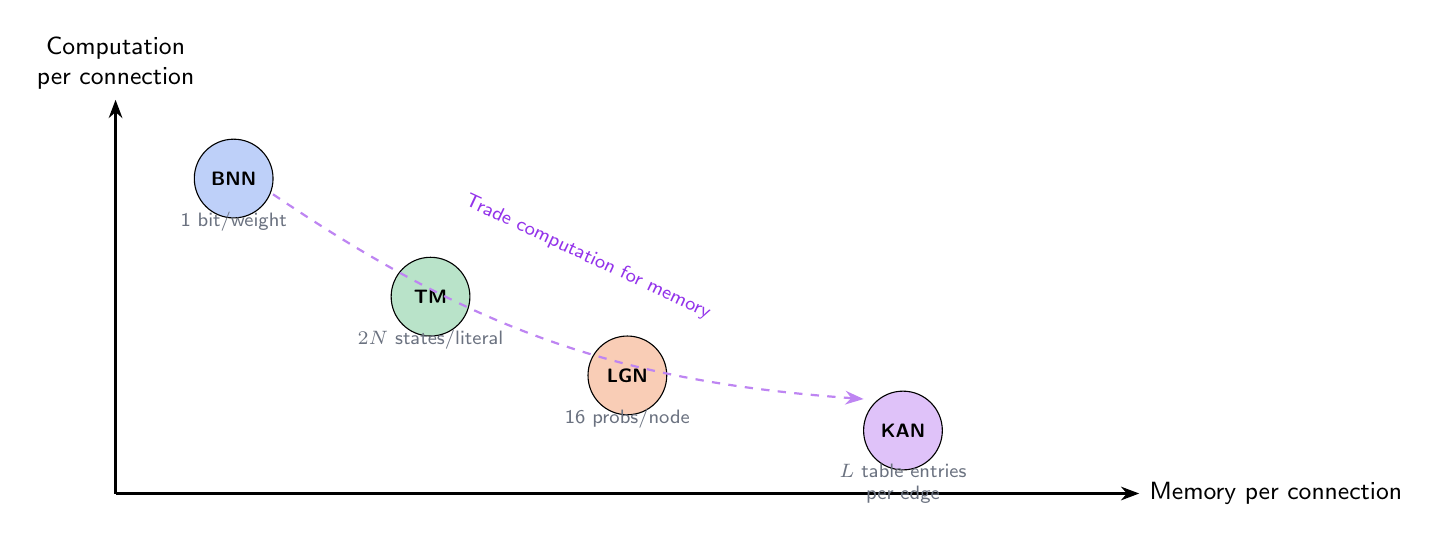
\begin{tikzpicture}[>=Stealth]
  % Axis
  \draw[->, thick] (0, 0) -- (13, 0)
    node[right, font=\small\sffamily] {Memory per connection};
  \draw[->, thick] (0, 0) -- (0, 5)
    node[above, font=\small\sffamily, align=center] {Computation\\per connection};

  % Paradigms
  \node[draw, circle, fill=bitblue!30, minimum size=1cm,
    font=\scriptsize\sffamily\bfseries] (bnn) at (1.5, 4) {BNN};
  \node[draw, circle, fill=bitgreen!30, minimum size=1cm,
    font=\scriptsize\sffamily\bfseries] (tm) at (4, 2.5) {TM};
  \node[draw, circle, fill=bitorange!30, minimum size=1cm,
    font=\scriptsize\sffamily\bfseries] (lgn) at (6.5, 1.5) {LGN};
  \node[draw, circle, fill=bitpurple!30, minimum size=1cm,
    font=\scriptsize\sffamily\bfseries] (kan) at (10, 0.8) {KAN};

  % Annotations
  \node[font=\scriptsize\sffamily, bitgray, below=0.3cm] at (bnn)
    {1 bit/weight};
  \node[font=\scriptsize\sffamily, bitgray, below=0.3cm] at (tm)
    {$2N$ states/literal};
  \node[font=\scriptsize\sffamily, bitgray, below=0.3cm] at (lgn)
    {16 probs/node};
  \node[font=\scriptsize\sffamily, bitgray, below=0.3cm, align=center]
    at (kan) {$L$ table entries\\per edge};

  % Trade-off arrow
  \draw[->, thick, dashed, bitpurple!60]
    (2, 3.8) to[bend right=15] (9.5, 1.2);
  \node[font=\scriptsize\sffamily, bitpurple, rotate=-25] at (6, 3)
    {Trade computation for memory};
\end{tikzpicture}
\caption{The computation--memory spectrum. Moving from BNNs to KAN/LUTs,
  each connection stores more information but requires less computation
  at inference time. This is the classic computer science trade-off
  applied to neural network design.}
\label{fig:compute-memory}
\end{figure}

% ============================================================================
\section{Toward a Hybrid Architecture}
\label{sec:hybrid}
% ============================================================================

The comparison in the previous section suggests that no single paradigm
is optimal across all criteria. This motivates a \concept{hybrid
architecture} that combines the strengths of multiple paradigms. This
section sketches a working hypothesis for such an architecture,
targeting MNIST~\cite{lecun1998mnist} as a proof of concept.

\subsection{Design Principles}

Our hybrid design is guided by four principles:

\begin{enumerate}[leftmargin=2em]
  \item \textbf{Interpretable feature extraction.} Use Tsetlin
    Machine clauses for the first stage: they learn human-readable
    rules about which pixel patterns indicate which digits.
  \item \textbf{Flexible composition.} Use Logic Gate Networks for
    the middle layers: they can learn complex combinations of the
    clause outputs using arbitrary logic gates.
  \item \textbf{Efficient deployment.} Use LUT compilation for
    any continuous functions that remain: compile learned activations
    into tables so that inference is pure memory access + bitwise
    logic.
  \item \textbf{All in Rust.} Implement both training and inference
    in Rust for speed, safety, and cross-platform deployment.
\end{enumerate}

\subsection{Proposed Architecture}

\begin{figure}[htbp]
\centering
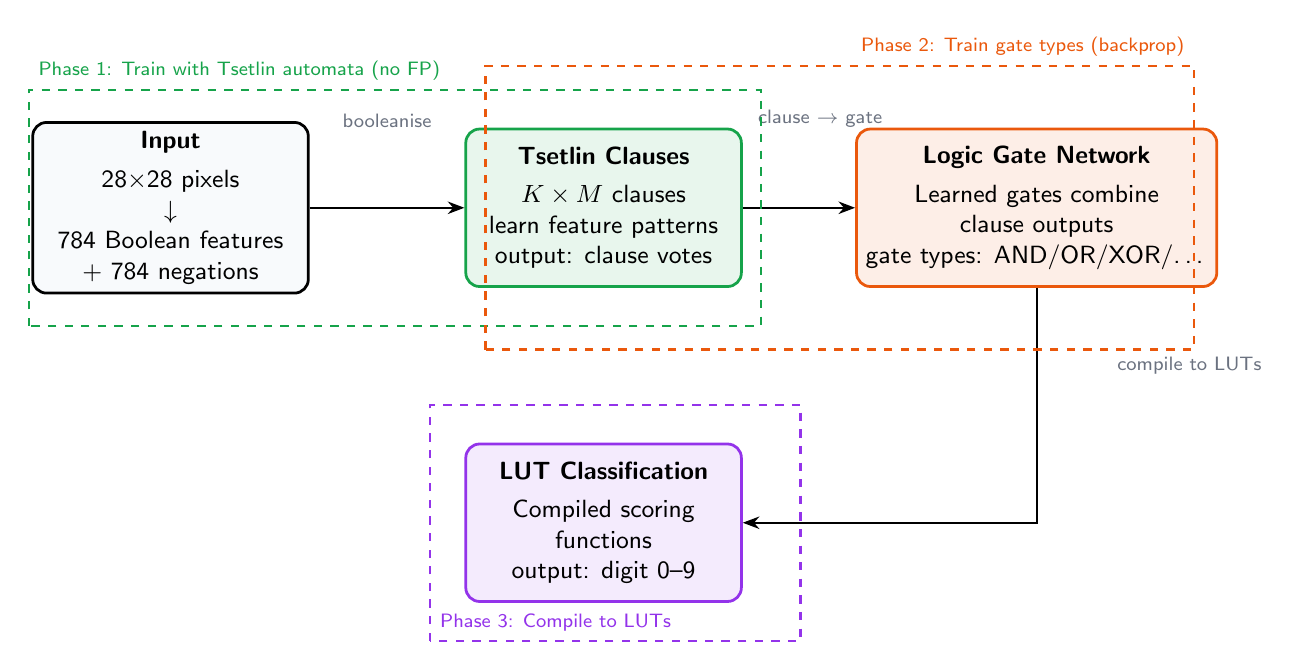
\begin{tikzpicture}[
  stage/.style={draw, rounded corners=5pt, minimum width=3.5cm,
    minimum height=2cm, align=center, font=\small\sffamily,
    line width=1pt},
  arr/.style={-{Stealth[length=6pt]}, thick},
  lbl/.style={font=\scriptsize\sffamily, bitgray}
]
  % Stage 1: Input
  \node[stage, fill=lightbg] (input) at (0, 0)
    {\textbf{Input}\\[3pt]28$\times$28 pixels\\$\downarrow$\\784 Boolean features\\+ 784 negations};

  % Stage 2: Tsetlin clauses
  \node[stage, fill=bitgreen!10, draw=bitgreen] (tm) at (5.5, 0)
    {\textbf{Tsetlin Clauses}\\[3pt]$K \times M$ clauses\\learn feature patterns\\output: clause votes};

  % Stage 3: LGN composition
  \node[stage, fill=bitorange!10, draw=bitorange] (lgn) at (11, 0)
    {\textbf{Logic Gate Network}\\[3pt]Learned gates combine\\clause outputs\\gate types: AND/OR/XOR/\ldots};

  % Stage 4: Output
  \node[stage, fill=bitpurple!10, draw=bitpurple] (out) at (5.5, -4)
    {\textbf{LUT Classification}\\[3pt]Compiled scoring\\functions\\output: digit 0--9};

  % Arrows
  \draw[arr] (input) -- (tm);
  \draw[arr] (tm) -- (lgn);
  \draw[arr] (lgn) |- (out);

  % Labels
  \node[lbl, above=0.1cm] at (2.75, 0.8)
    {booleanise};
  \node[lbl, above=0.1cm] at (8.25, 0.8)
    {clause $\to$ gate};
  \node[lbl, right=0.1cm] at (11.8, -2)
    {compile to LUTs};

  % Training annotations
  \draw[dashed, bitgreen, thick] (-1.8, -1.5) rectangle (7.5, 1.5);
  \node[font=\scriptsize\sffamily, bitgreen, anchor=south west]
    at (-1.8, 1.5) {Phase 1: Train with Tsetlin automata (no FP)};

  \draw[dashed, bitorange, thick] (4, -1.8) rectangle (13, 1.8);
  \node[font=\scriptsize\sffamily, bitorange, anchor=south east]
    at (13, 1.8) {Phase 2: Train gate types (backprop)};

  \draw[dashed, bitpurple, thick] (3.3, -5.5) rectangle (8, -2.5);
  \node[font=\scriptsize\sffamily, bitpurple, anchor=south west]
    at (3.3, -5.5) {Phase 3: Compile to LUTs};
\end{tikzpicture}
\caption{Proposed hybrid architecture. Stage 1 (Tsetlin) learns
  interpretable feature patterns. Stage 2 (LGN) composes patterns with
  learned logic gates. Stage 3 (LUT) compiles any remaining scoring
  functions into lookup tables. Training is phased: Tsetlin automata
  first (no floating-point needed), then backpropagation for gate
  learning, then one-time LUT compilation.}
\label{fig:hybrid-architecture}
\end{figure}

\subsection{Training Pipeline}

The hybrid architecture suggests a three-phase training pipeline:

\begin{description}[leftmargin=1em]
  \item[Phase 1: Clause learning (Tsetlin).]
    Train the Tsetlin Machine component on the booleanised MNIST
    inputs. This produces a set of interpretable clauses---Boolean
    expressions that capture local pixel patterns. The output of this
    phase is a fixed set of clause activations per input image.
    \emph{No floating-point arithmetic required.}

  \item[Phase 2: Gate learning (LGN).]
    Freeze the Tsetlin clauses. Train a Logic Gate Network on top
    of the clause outputs. The LGN learns which gate types and
    connectivity best combine the clause features into class scores.
    This phase uses standard backpropagation with softmax relaxation
    and temperature annealing.

  \item[Phase 3: LUT compilation.]
    After gate types are committed, compile any remaining continuous
    functions (e.g., scoring aggregation, temperature scaling) into
    lookup tables. The final inference model is entirely
    integer/Boolean.
\end{description}

\begin{engineernote}
This phased approach has a practical advantage for Rust
implementation: Phase~1 needs only integer operations and random
number generation. Phase~2 needs floating-point backpropagation
(the most complex part). Phase~3 is a one-time offline step.
You can implement and test each phase independently.
\end{engineernote}

\subsection{Expected Characteristics}

\begin{table}[htbp]
\centering
\caption{Expected characteristics of the hybrid architecture on MNIST
  (estimates based on component performance).}
\label{tab:hybrid-expected}
\begin{tabular}{@{}lr@{}}
  \toprule
  \textbf{Metric} & \textbf{Expected Range} \\
  \midrule
  Accuracy          & 97--99\% \\
  Model size         & 50--500\,kB \\
  Inference ops      & Boolean + LUT only \\
  FP at inference?   & No \\
  Interpretability   & Partial (Tsetlin clauses readable) \\
  \bottomrule
\end{tabular}
\end{table}

\subsection{Benchmarking Plan}

To validate the hybrid approach, we will benchmark against a standard
floating-point baseline:

\begin{enumerate}[leftmargin=2em]
  \item \textbf{Baseline model:} A standard 2-layer MLP with ReLU
    activations, trained with Adam optimiser in 32-bit floating
    point. Expected accuracy: $\sim$98\%.
  \item \textbf{Metrics:}
    \begin{itemize}[leftmargin=1em]
      \item Classification accuracy (test set)
      \item Inference latency (microseconds per image)
      \item Model size (bytes)
      \item Inference energy estimate (based on operation counts)
    \end{itemize}
  \item \textbf{Environment:} Both models implemented in Rust, running
    on the same CPU, with no GPU acceleration for either.
\end{enumerate}

% ============================================================================
\section{Understanding Transformers and Large Language Models}
\label{sec:transformers-llms}
% ============================================================================

The previous sections developed four paradigms for replacing
floating-point arithmetic with bitwise operations, and showed how they
combine into a hybrid architecture for MNIST. Before we can honestly
evaluate whether any of this scales to large language models (LLMs),
we need to understand what LLMs actually \emph{are}---what makes them
work, and which of their components are essential versus replaceable.

This section builds that understanding from the ground up, using the
same intuition-first approach as the rest of this article.

% ----------------------------------------------------------------------------
\subsection{From Pixels to Words: Why Language Is Harder}
\label{sec:pixels-vs-words}
% ----------------------------------------------------------------------------

MNIST is a \emph{fixed-size classification} problem: 784 pixels in,
one of ten labels out. Every input has the same shape, and every pixel
has a clear spatial relationship to its neighbours.

Language is fundamentally different:

\begin{itemize}[leftmargin=2em]
  \item \textbf{Variable length.} A sentence can be 5~words or
    5{,}000~words. The network must handle both.
  \item \textbf{No fixed grid.} Words are not arranged in a 2D grid
    like pixels. Their meaning depends on \emph{order} and
    \emph{context}---``the dog bit the man'' and ``the man bit the
    dog'' use the same words but mean different things.
  \item \textbf{Long-range dependencies.} In ``The cat that the dog
    chased ran away,'' the verb ``ran'' relates to ``cat,'' not the
    nearby ``dog.'' The network must connect words across arbitrary
    distances.
  \item \textbf{Generation, not classification.} An LLM does not pick
    one of ten labels. It generates text one word at a time, choosing
    from a vocabulary of 30{,}000--100{,}000 possible next words at
    each step.
\end{itemize}

\begin{keyinsight}
The transition from MNIST to language is not just ``bigger data.'' It
requires fundamentally different architectural primitives: a way to
represent words as numbers, a mechanism to relate words to each other
regardless of distance, and a method for generating sequences one
element at a time.
\end{keyinsight}

% ----------------------------------------------------------------------------
\subsection{Tokenisation: Turning Text into Numbers}
\label{sec:tokenisation}
% ----------------------------------------------------------------------------

A neural network cannot process letters or words directly---it needs
numbers. The first step in any language model is \concept{tokenisation}:
splitting text into small pieces and assigning each piece an integer ID.

Modern LLMs do not split on whole words. Instead, they use
\concept{subword tokenisation} (algorithms like Byte-Pair Encoding or
SentencePiece), which breaks text into frequently occurring fragments:

\begin{figure}[htbp]
\centering
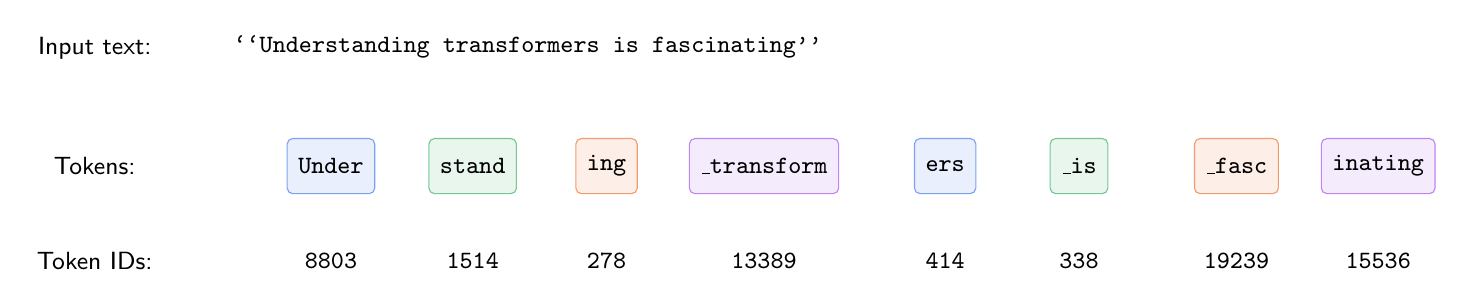
\begin{tikzpicture}[
  tok/.style={draw, rounded corners=2pt, minimum height=0.7cm,
    font=\small\ttfamily, inner sep=4pt, fill=#1!10, draw=#1!60},
  arr/.style={-{Stealth[length=4pt]}, thick, bitgray}
]
  % Original text
  \node[font=\small\sffamily] at (-1.5, 1.5) {Input text:};
  \node[font=\small\ttfamily] at (4, 1.5)
    {``Understanding transformers is fascinating''};

  % Tokens
  \node[font=\small\sffamily] at (-1.5, 0) {Tokens:};
  \node[tok=bitblue]   (t1) at (1.5, 0) {Under};
  \node[tok=bitgreen]  (t2) at (3.3, 0) {stand};
  \node[tok=bitorange] (t3) at (5.0, 0) {ing};
  \node[tok=bitpurple] (t4) at (7.0, 0) {\_transform};
  \node[tok=bitblue]   (t5) at (9.3, 0) {ers};
  \node[tok=bitgreen]  (t6) at (11.0, 0) {\_is};
  \node[tok=bitorange] (t7) at (13.0, 0) {\_fasc};
  \node[tok=bitpurple] (t8) at (14.8, 0) {inating};

  % Token IDs
  \node[font=\small\sffamily] at (-1.5, -1.2) {Token IDs:};
  \node[font=\small\ttfamily] at (1.5, -1.2) {8803};
  \node[font=\small\ttfamily] at (3.3, -1.2) {1514};
  \node[font=\small\ttfamily] at (5.0, -1.2) {278};
  \node[font=\small\ttfamily] at (7.0, -1.2) {13389};
  \node[font=\small\ttfamily] at (9.3, -1.2) {414};
  \node[font=\small\ttfamily] at (11.0, -1.2) {338};
  \node[font=\small\ttfamily] at (13.0, -1.2) {19239};
  \node[font=\small\ttfamily] at (14.8, -1.2) {15536};
\end{tikzpicture}
\caption{Subword tokenisation splits text into frequently occurring
  fragments, each mapped to an integer ID. Common words become single
  tokens; rare words are split into subwords. The underscore
  (\_) represents a space preceding the token.}
\label{fig:tokenisation}
\end{figure}

\begin{analogy}
Tokenisation is like Morse code for neural networks. Just as Morse
represents each letter as a sequence of dots and dashes, tokenisation
represents each text fragment as a number. The difference is that the
``alphabet'' is learned from data: common fragments (``the'', ``ing'',
``tion'') get their own codes, while rare fragments are spelled out
from smaller pieces. A typical LLM vocabulary has 30{,}000--100{,}000
tokens.
\end{analogy}

The key property is that \emph{any} text can be represented as a
sequence of token IDs. The model's input is always a sequence of
integers: $[t_1, t_2, \ldots, t_n]$ where each $t_i \in
\{0, 1, \ldots, V{-}1\}$ and $V$ is the vocabulary size.

% ----------------------------------------------------------------------------
\subsection{Embeddings: Words as Points in Space}
\label{sec:embeddings}
% ----------------------------------------------------------------------------

A token ID like 13389 is just a number---it tells us nothing about
what the token \emph{means}. The next step is to convert each token
into a \concept{high-dimensional vector}, called an
\concept{embedding}.

An embedding is a list of numbers (typically 768 to 4{,}096 of them)
that represents the token as a point in a high-dimensional space. The
critical property is that tokens with similar meanings end up at
nearby points:

\begin{figure}[htbp]
\centering
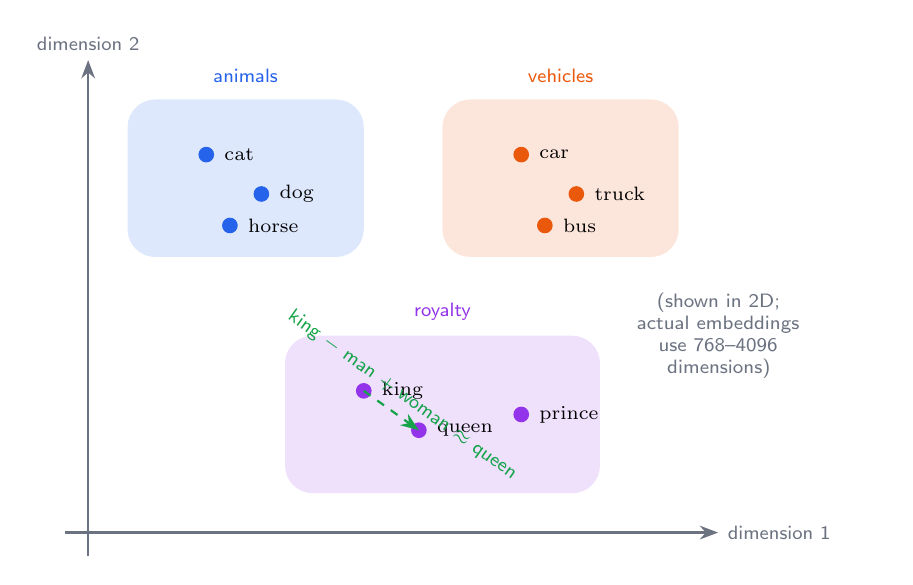
\begin{tikzpicture}[scale=1.0]
  % Axes
  \draw[-{Stealth}, thick, bitgray] (-0.3, 0) -- (8, 0);
  \draw[-{Stealth}, thick, bitgray] (0, -0.3) -- (0, 6);
  \node[font=\scriptsize\sffamily, bitgray, right] at (8, 0)
    {dimension 1};
  \node[font=\scriptsize\sffamily, bitgray, above] at (0, 6)
    {dimension 2};

  % Animal cluster
  \fill[bitblue!15, rounded corners=10pt]
    (0.5, 3.5) rectangle (3.5, 5.5);
  \node[font=\scriptsize\sffamily, bitblue] at (2, 5.8) {animals};
  \node[circle, fill=bitblue, inner sep=2pt, label={[font=\scriptsize]right:cat}]
    at (1.5, 4.8) {};
  \node[circle, fill=bitblue, inner sep=2pt, label={[font=\scriptsize]right:dog}]
    at (2.2, 4.3) {};
  \node[circle, fill=bitblue, inner sep=2pt, label={[font=\scriptsize]right:horse}]
    at (1.8, 3.9) {};

  % Vehicle cluster
  \fill[bitorange!15, rounded corners=10pt]
    (4.5, 3.5) rectangle (7.5, 5.5);
  \node[font=\scriptsize\sffamily, bitorange] at (6, 5.8) {vehicles};
  \node[circle, fill=bitorange, inner sep=2pt, label={[font=\scriptsize]right:car}]
    at (5.5, 4.8) {};
  \node[circle, fill=bitorange, inner sep=2pt, label={[font=\scriptsize]right:truck}]
    at (6.2, 4.3) {};
  \node[circle, fill=bitorange, inner sep=2pt, label={[font=\scriptsize]right:bus}]
    at (5.8, 3.9) {};

  % Royalty cluster
  \fill[bitpurple!15, rounded corners=10pt]
    (2.5, 0.5) rectangle (6.5, 2.5);
  \node[font=\scriptsize\sffamily, bitpurple] at (4.5, 2.8) {royalty};
  \node[circle, fill=bitpurple, inner sep=2pt, label={[font=\scriptsize]right:king}]
    at (3.5, 1.8) {};
  \node[circle, fill=bitpurple, inner sep=2pt, label={[font=\scriptsize]right:queen}]
    at (4.2, 1.3) {};
  \node[circle, fill=bitpurple, inner sep=2pt, label={[font=\scriptsize]right:prince}]
    at (5.5, 1.5) {};

  % Analogy arrow
  \draw[-{Stealth}, thick, dashed, bitgreen]
    (3.5, 1.8) -- node[font=\scriptsize\sffamily, above, sloped]
    {king $-$ man $+$ woman $\approx$ queen} (4.2, 1.3);

  % Note
  \node[font=\scriptsize\sffamily, bitgray, text width=4cm, align=center]
    at (8, 2.5) {(shown in 2D;\\actual embeddings\\use 768--4096\\dimensions)};
\end{tikzpicture}
\caption{Token embeddings place words in a high-dimensional space
  where distance reflects semantic similarity. Similar words cluster
  together, and vector arithmetic can capture analogies.
  This picture is simplified to 2D; real embeddings use hundreds to
  thousands of dimensions.}
\label{fig:embeddings}
\end{figure}

\begin{engineernote}
An embedding table is conceptually simple: it is a 2D array of shape
$V \times d$, where $V$ is the vocabulary size and $d$ is the
embedding dimension. Looking up a token's embedding is a single
table lookup---no computation, just a memory read of $d$ numbers.
In a model with $V = 50{,}000$ and $d = 4{,}096$, the embedding
table alone uses $50{,}000 \times 4{,}096 \times 2 = 400$\,MB
(in 16-bit precision).
\end{engineernote}

The embedding is not fixed forever. The embedding table is \emph{learned}
during training: the model adjusts the position of every token in this
high-dimensional space so that tokens appearing in similar contexts
end up nearby. This learned structure is called \concept{distributional
semantics}---the meaning of a word is defined by the company it keeps.

\subsubsection{Why High Dimensions Matter}

Two dimensions can separate cats from cars. But to simultaneously
encode that ``bank'' can mean a financial institution \emph{or} a
river bank, that ``run'' can be a verb \emph{or} a noun, and that
``Java'' can be a programming language \emph{or} an island---you need
many dimensions. Each dimension can encode a different aspect of
meaning, and a token's position in this space encodes all its
potential meanings simultaneously.

This is the first point of tension with bitwise approaches:
\emph{embeddings are inherently continuous}. The difference between
``happy'' and ``joyful'' is a small vector in this space; booleanising
it (rounding each dimension to 0 or~1) would destroy these fine
distinctions.

% ----------------------------------------------------------------------------
\subsection{The Transformer Block: The Engine of Modern AI}
\label{sec:transformer-block}
% ----------------------------------------------------------------------------

The transformer~\cite{vaswani2017attention} is the architecture
behind essentially all modern LLMs (GPT, Claude, Llama, etc.). A
transformer is a stack of identical \concept{transformer blocks}, each
containing two main sub-layers:

\begin{enumerate}[leftmargin=2em]
  \item \textbf{Self-attention}: lets each token look at every other
    token and decide which ones are relevant.
  \item \textbf{Feed-forward network (MLP)}: processes each token
    independently through a small neural network.
\end{enumerate}

Each sub-layer is wrapped in a \concept{residual connection} (add the
input back to the output) and \concept{layer normalisation} (rescale
the values to prevent them from growing too large or too small).

\begin{figure}[htbp]
\centering
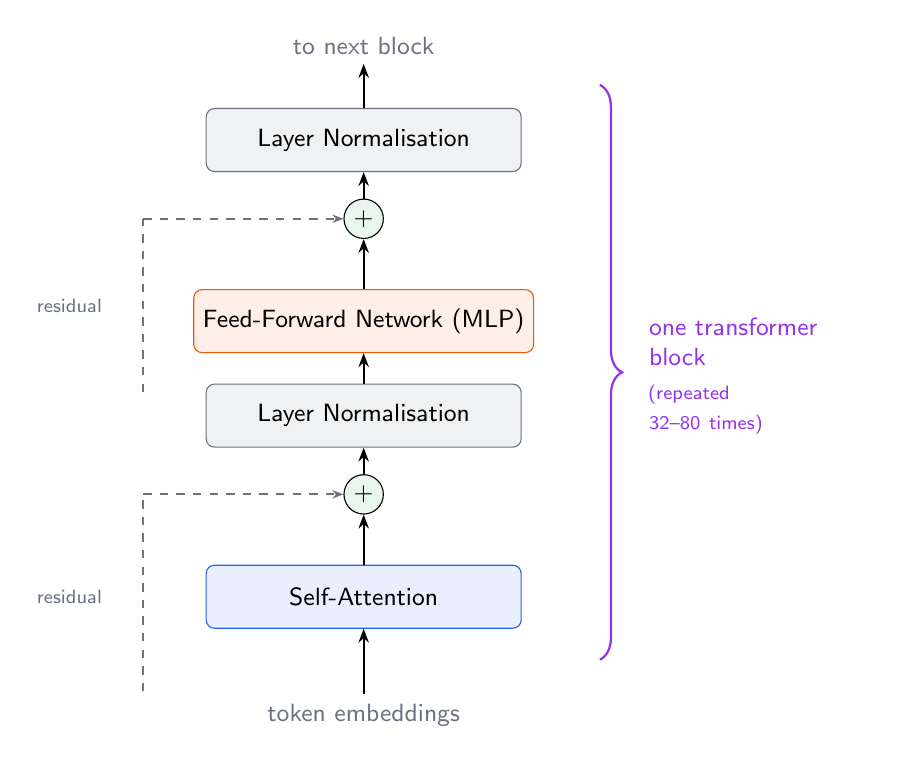
\begin{tikzpicture}[
  block/.style={draw, rounded corners=3pt, minimum width=4cm,
    minimum height=0.8cm, font=\small\sffamily, align=center},
  arr/.style={-{Stealth[length=5pt]}, thick},
  plus/.style={circle, draw, minimum size=0.5cm, font=\small,
    fill=bitgreen!10, inner sep=0pt},
  skip/.style={thick, bitgray, dashed}
]
  % Input
  \node[font=\small\sffamily, bitgray] (in) at (0, 0) {token embeddings};

  % Self-attention
  \node[block, fill=bitblue!10, draw=bitblue] (attn)
    at (0, 1.5) {Self-Attention};
  \node[plus] (add1) at (0, 2.8) {$+$};
  \node[block, fill=bitgray!10, draw=bitgray] (ln1)
    at (0, 3.8) {Layer Normalisation};

  % MLP
  \node[block, fill=bitorange!10, draw=bitorange] (mlp)
    at (0, 5.0) {Feed-Forward Network (MLP)};
  \node[plus] (add2) at (0, 6.3) {$+$};
  \node[block, fill=bitgray!10, draw=bitgray] (ln2)
    at (0, 7.3) {Layer Normalisation};

  % Output
  \node[font=\small\sffamily, bitgray] (out) at (0, 8.5)
    {to next block};

  % Main flow
  \draw[arr] (in) -- (attn);
  \draw[arr] (attn) -- (add1);
  \draw[arr] (add1) -- (ln1);
  \draw[arr] (ln1) -- (mlp);
  \draw[arr] (mlp) -- (add2);
  \draw[arr] (add2) -- (ln2);
  \draw[arr] (ln2) -- (out);

  % Residual connections
  \draw[skip] (-2.8, 0.3) -- (-2.8, 2.8);
  \draw[skip, -{Stealth[length=4pt]}] (-2.8, 2.8) -- (add1);
  \draw[skip] (-2.8, 4.1) -- (-2.8, 6.3);
  \draw[skip, -{Stealth[length=4pt]}] (-2.8, 6.3) -- (add2);

  % Labels
  \node[font=\scriptsize\sffamily, bitgray, left] at (-3.2, 1.5)
    {residual};
  \node[font=\scriptsize\sffamily, bitgray, left] at (-3.2, 5.2)
    {residual};

  % Bracket for "one block"
  \draw[decorate, decoration={brace, amplitude=8pt, mirror},
    thick, bitpurple]
    (3, 0.7) -- (3, 8.0);
  \node[font=\small\sffamily, bitpurple, right, text width=3cm]
    at (3.5, 4.3)
    {one transformer\\block\\[4pt]\scriptsize (repeated\\32--80 times)};
\end{tikzpicture}
\caption{A single transformer block. The self-attention sub-layer lets
  tokens communicate with each other; the MLP sub-layer processes each
  token independently. Residual connections and layer normalisation
  stabilise training. A full LLM stacks 32--80 of these blocks.}
\label{fig:transformer-block}
\end{figure}

\begin{analogy}
Think of a transformer block as a two-step meeting process. In the
\emph{self-attention} step, every participant in the room looks
around, identifies who has relevant information, and takes notes.
In the \emph{MLP} step, each participant goes back to their desk
and privately thinks about what they learned. Then the whole process
repeats---another round of group discussion followed by private
reflection. After 32--80 rounds, each participant has a rich
understanding of the entire conversation.

The residual connection is like keeping your original notes alongside
the new ones---you never lose what you started with. Layer
normalisation is like agreeing on a common scale for everyone's
notes so that one loud participant does not dominate.
\end{analogy}

Let us examine each component in detail.

% ----------------------------------------------------------------------------
\subsection{Self-Attention: The Core Innovation}
\label{sec:self-attention}
% ----------------------------------------------------------------------------

Self-attention is the mechanism that lets each token in a sequence
attend to every other token. It answers the question: \emph{``For each
word I am processing, which other words in the sequence should
influence my understanding of it?''}

\subsubsection{The Intuition}

Consider the sentence: ``The animal didn't cross the street because
it was too wide.'' What does ``it'' refer to? A human instantly knows
``it'' means ``the street'' (streets are wide, not animals). But how
does a neural network figure this out?

Self-attention lets the token ``it'' \emph{look at every other token}
and assign each one a relevance score. It assigns high relevance to
``street'' and low relevance to ``animal,'' then uses these scores to
blend information from the relevant tokens into its own representation.

\subsubsection{The Mechanism: Queries, Keys, and Values}

Self-attention works through three learned projections. For each token,
the model computes:

\begin{itemize}[leftmargin=2em]
  \item A \concept{query} ($\bm{q}$): ``What am I looking for?''
  \item A \concept{key} ($\bm{k}$): ``What do I contain?''
  \item A \concept{value} ($\bm{v}$): ``What information do I
    provide if selected?''
\end{itemize}

\begin{figure}[htbp]
\centering
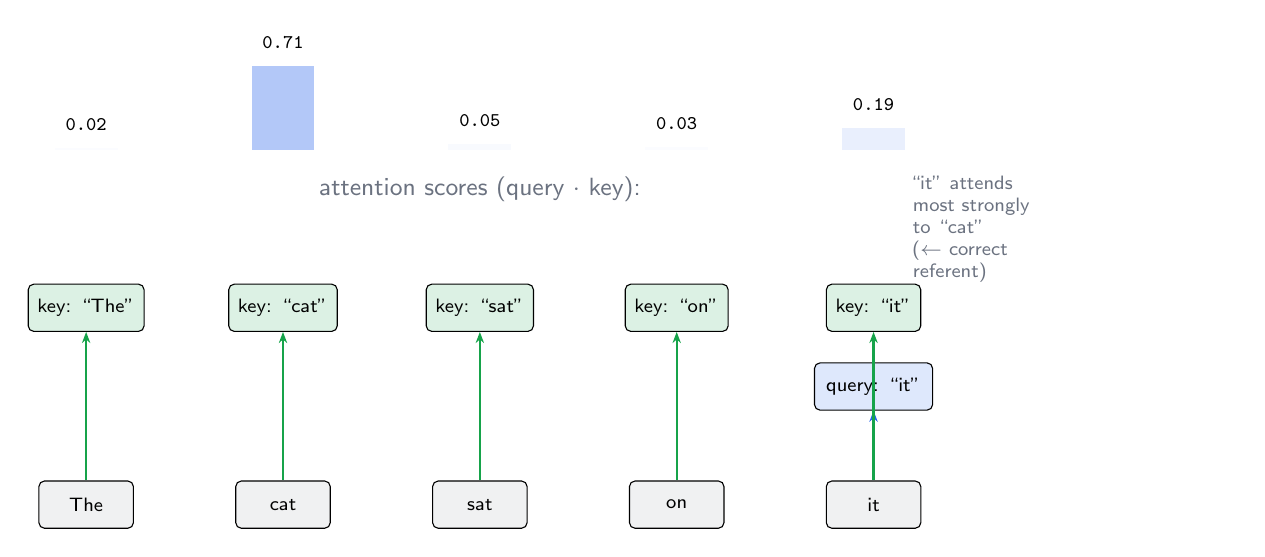
\begin{tikzpicture}[
  tok/.style={draw, rounded corners=2pt, minimum width=1.2cm,
    minimum height=0.6cm, font=\scriptsize\sffamily, fill=#1!10},
  mat/.style={draw, rounded corners=2pt, minimum width=1cm,
    minimum height=0.6cm, font=\scriptsize\sffamily, fill=#1!15},
  arr/.style={-{Stealth[length=4pt]}, thick},
  score/.style={font=\scriptsize\ttfamily}
]
  % Tokens
  \foreach \i/\w in {1/The, 2/cat, 3/sat, 4/on, 5/it} {
    \node[tok=bitgray] (t\i) at ({(\i-1)*2.5}, 0) {\w};
  }

  % Query from "it"
  \node[mat=bitblue, minimum width=1.5cm] (q) at (10, 1.5)
    {query: ``it''};
  \draw[arr, bitblue] (t5.north) -- (q.south);

  % Keys from all
  \foreach \i/\w in {1/The, 2/cat, 3/sat, 4/on, 5/it} {
    \node[mat=bitgreen] (k\i) at ({(\i-1)*2.5}, 2.5)
      {key: ``\w''};
    \draw[arr, bitgreen] (t\i.north) -- (k\i.south);
  }

  % Attention scores
  \node[font=\small\sffamily, bitgray] at (5, 4) {attention scores
    (query $\cdot$ key):};
  \foreach \i/\s/\h in {1/0.02/2, 2/0.71/35, 3/0.05/3, 4/0.03/2, 5/0.19/10} {
    \fill[bitblue!\h] ({(\i-1)*2.5-0.4}, 4.5) rectangle
      ({(\i-1)*2.5+0.4}, {4.5+\s*1.5});
    \node[score] at ({(\i-1)*2.5}, {4.5+\s*1.5+0.3}) {\s};
  }

  % Label
  \node[font=\scriptsize\sffamily, bitgray, text width=4cm, align=left]
    at (12.5, 3.5) {``it'' attends\\most strongly\\to ``cat''\\($\leftarrow$ correct\\referent)};
\end{tikzpicture}
\caption{Self-attention for the token ``it''. Its query is compared
  (via dot product) with every token's key to produce attention scores.
  The highest score (0.71) goes to ``cat''---the token ``it'' refers to.
  These scores then weight each token's value to produce the output.}
\label{fig:attention-scores}
\end{figure}

\subsubsection{The Mathematics}

Given a sequence of $n$ token embeddings packed into a matrix
$\bm{X} \in \mathbb{R}^{n \times d}$, self-attention computes:

\begin{align}
  \bm{Q} &= \bm{X}\bm{W}_Q, \quad
  \bm{K} = \bm{X}\bm{W}_K, \quad
  \bm{V} = \bm{X}\bm{W}_V
  \label{eq:qkv}\\[6pt]
  \text{Attention}(\bm{Q}, \bm{K}, \bm{V})
  &= \underbrace{\text{softmax}\!\left(
    \frac{\bm{Q}\bm{K}^\top}{\sqrt{d_k}}
  \right)}_{\text{attention weights}}
  \bm{V}
  \label{eq:attention}
\end{align}

where $\bm{W}_Q, \bm{W}_K, \bm{W}_V \in \mathbb{R}^{d \times d_k}$
are learned projection matrices, and $d_k$ is the dimension of each
head (typically $d / h$ where $h$ is the number of attention heads).

Let us unpack each step:

\begin{enumerate}[leftmargin=2em]
  \item \textbf{Project.} Multiply the input by three weight matrices
    to get queries, keys, and values. This is standard matrix
    multiplication---the same MAC operation we have been trying to
    eliminate.

  \item \textbf{Score.} Compute $\bm{Q}\bm{K}^\top$: the dot product
    of every query with every key. This produces an $n \times n$
    matrix of raw relevance scores. For a sequence of 4{,}096 tokens,
    this is a $4{,}096 \times 4{,}096$ matrix---about 16~million
    scores.

  \item \textbf{Scale.} Divide by $\sqrt{d_k}$ to prevent the dot
    products from growing too large (which would push softmax into
    regions where its gradient vanishes).

  \item \textbf{Softmax.} Apply the softmax function to each row:
    \begin{equation}
      \text{softmax}(z_i) = \frac{e^{z_i}}{\sum_j e^{z_j}}
      \label{eq:softmax}
    \end{equation}
    This converts raw scores into a probability distribution: all
    positive, summing to~1. The token with the highest relevance
    gets the most weight.

  \item \textbf{Aggregate.} Multiply the attention weights by the
    value matrix. Each token's output is a weighted average of all
    tokens' values, where the weights reflect relevance.
\end{enumerate}

\begin{keyinsight}
The softmax function is the critical bottleneck for binarisation.
It requires:
\begin{itemize}[leftmargin=1em]
  \item Exponentiation ($e^{z_i}$)---a transcendental function that
    maps integers to irrational numbers.
  \item Division---to normalise the probabilities.
  \item Continuous outputs---the weights 0.71 and 0.72 must be
    distinguishable, not rounded to the same bit.
\end{itemize}
Every other step (projection, scoring, aggregation) is matrix
multiplication, which \emph{can} be approximated with integer or
ternary arithmetic (as BitNet demonstrates). The softmax is where
floating-point computation concentrates.
\end{keyinsight}

\subsubsection{Multi-Head Attention}

In practice, the model does not compute one set of queries, keys, and
values. It computes $h$ sets in parallel (typically $h = 32$ to 128),
each with a smaller dimension $d_k = d/h$. These are called
\concept{attention heads}.

\begin{analogy}
Multi-head attention is like having multiple reading comprehension
specialists. One head might focus on syntactic relationships (subject
and verb agreement), another on semantic similarity (synonyms and
related concepts), a third on positional relationships (nearby words).
Each head independently decides what is relevant, and their
conclusions are concatenated and combined.
\end{analogy}

The output of multi-head attention is:
\begin{equation}
  \text{MultiHead}(\bm{X}) =
  [\text{head}_1; \text{head}_2; \ldots; \text{head}_h]\bm{W}_O
\end{equation}
where each $\text{head}_i = \text{Attention}(\bm{X}\bm{W}_Q^i,
\bm{X}\bm{W}_K^i, \bm{X}\bm{W}_V^i)$ and $\bm{W}_O \in
\mathbb{R}^{d \times d}$ is a learned output projection.

% ----------------------------------------------------------------------------
\subsection{The Feed-Forward Network (MLP Block)}
\label{sec:ffn}
% ----------------------------------------------------------------------------

After attention lets tokens communicate, each token is processed
\emph{independently} through a small two-layer neural network:

\begin{equation}
  \text{FFN}(\bm{x}) = \sigma(\bm{x}\bm{W}_1 + \bm{b}_1)\bm{W}_2 + \bm{b}_2
  \label{eq:ffn}
\end{equation}

where $\sigma$ is a nonlinear activation function (typically GELU or
SiLU), $\bm{W}_1 \in \mathbb{R}^{d \times d_{\text{ff}}}$ and
$\bm{W}_2 \in \mathbb{R}^{d_{\text{ff}} \times d}$.

The inner dimension $d_{\text{ff}}$ is typically $4 \times d$. For a
model with $d = 4{,}096$, this means $\bm{W}_1$ has $4{,}096 \times
16{,}384 = 67$~million parameters---\emph{per layer}.

\begin{engineernote}
The MLP block is where most of the model's parameters and computation
live. In a typical transformer, the MLP accounts for about two-thirds
of the total parameters and floating-point operations. This makes it
the highest-value target for binarisation: if you can make the MLP
bitwise, you have eliminated the majority of the floating-point work.
\end{engineernote}

\begin{analogy}
If self-attention is the ``group discussion'' where tokens share
information, the MLP is the ``private thinking'' where each token
processes what it learned. The attention layer moves information
\emph{between} tokens; the MLP transforms information \emph{within}
each token.
\end{analogy}

% ----------------------------------------------------------------------------
\subsection{Residual Connections and Layer Normalisation}
\label{sec:residual-layernorm}
% ----------------------------------------------------------------------------

Two seemingly minor components turn out to be essential for making
deep transformers trainable.

\subsubsection{Residual Connections}

A residual connection simply adds the input of a sub-layer back to
its output:
\begin{equation}
  \bm{y} = \bm{x} + \text{SubLayer}(\bm{x})
  \label{eq:residual}
\end{equation}

This means the sub-layer only needs to learn the \emph{difference}
from the input, not the entire transformation. Without residual
connections, gradients vanish in deep networks---a 96-layer
transformer would be untrainable.

\subsubsection{Layer Normalisation}

Layer normalisation~\cite{ba2016layernorm} rescales each token's
representation to have zero mean and unit variance:
\begin{equation}
  \text{LayerNorm}(\bm{x}) =
  \frac{\bm{x} - \mu}{\sqrt{\sigma^2 + \epsilon}} \odot \bm{\gamma} + \bm{\beta}
  \label{eq:layernorm}
\end{equation}
where $\mu$ and $\sigma^2$ are the mean and variance computed across
the embedding dimensions of a single token, $\bm{\gamma}$ and
$\bm{\beta}$ are learned scale and shift parameters, and $\epsilon$
is a small constant for numerical stability.

\begin{engineernote}
Layer normalisation is another floating-point bottleneck. It requires:
\begin{itemize}[leftmargin=1em]
  \item Computing mean and variance (requires division and square root).
  \item The division $(\bm{x} - \mu) / \sqrt{\sigma^2 + \epsilon}$
    produces continuous values even if $\bm{x}$ is integer.
  \item The learned parameters $\bm{\gamma}$ and $\bm{\beta}$ are
    continuous.
\end{itemize}
However, approximations exist: \concept{RMSNorm} (used in Llama and
many modern LLMs) drops the mean subtraction and simplifies to
$\bm{x} / \text{RMS}(\bm{x}) \cdot \bm{\gamma}$, which is slightly
simpler. Integer approximations of RMSNorm have been demonstrated
in quantisation research, though with some accuracy trade-off.
\end{engineernote}

% ----------------------------------------------------------------------------
\subsection{Autoregressive Generation: One Token at a Time}
\label{sec:autoregressive}
% ----------------------------------------------------------------------------

An LLM generates text through \concept{autoregressive generation}:
it predicts the next token, appends it to the sequence, and repeats.

\begin{figure}[htbp]
\centering
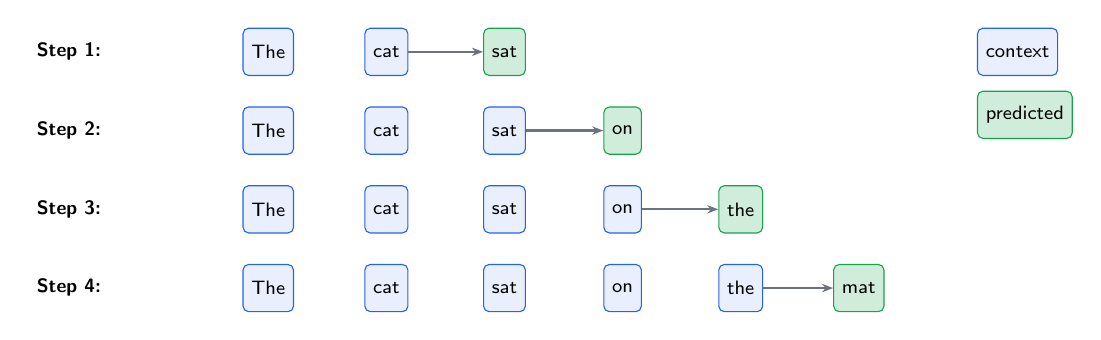
\begin{tikzpicture}[
  tok/.style={draw, rounded corners=2pt, minimum height=0.6cm,
    font=\scriptsize\sffamily, inner sep=3pt},
  pred/.style={tok, fill=bitgreen!20, draw=bitgreen},
  ctx/.style={tok, fill=bitblue!10, draw=bitblue},
  arr/.style={-{Stealth[length=4pt]}, thick, bitgray}
]
  % Step 1
  \node[font=\scriptsize\sffamily\bfseries, left] at (-0.5, 3)
    {Step 1:};
  \node[ctx] (s1a) at (1.5, 3) {The};
  \node[ctx] (s1b) at (3, 3) {cat};
  \node[pred] (s1c) at (4.5, 3) {sat};
  \draw[arr] (s1b) -- (s1c);

  % Step 2
  \node[font=\scriptsize\sffamily\bfseries, left] at (-0.5, 2)
    {Step 2:};
  \node[ctx] (s2a) at (1.5, 2) {The};
  \node[ctx] (s2b) at (3, 2) {cat};
  \node[ctx] (s2c) at (4.5, 2) {sat};
  \node[pred] (s2d) at (6, 2) {on};
  \draw[arr] (s2c) -- (s2d);

  % Step 3
  \node[font=\scriptsize\sffamily\bfseries, left] at (-0.5, 1)
    {Step 3:};
  \node[ctx] (s3a) at (1.5, 1) {The};
  \node[ctx] (s3b) at (3, 1) {cat};
  \node[ctx] (s3c) at (4.5, 1) {sat};
  \node[ctx] (s3d) at (6, 1) {on};
  \node[pred] (s3e) at (7.5, 1) {the};
  \draw[arr] (s3d) -- (s3e);

  % Step 4
  \node[font=\scriptsize\sffamily\bfseries, left] at (-0.5, 0)
    {Step 4:};
  \node[ctx] (s4a) at (1.5, 0) {The};
  \node[ctx] (s4b) at (3, 0) {cat};
  \node[ctx] (s4c) at (4.5, 0) {sat};
  \node[ctx] (s4d) at (6, 0) {on};
  \node[ctx] (s4e) at (7.5, 0) {the};
  \node[pred] (s4f) at (9, 0) {mat};
  \draw[arr] (s4e) -- (s4f);

  % Legend
  \node[ctx, right] at (10.5, 3) {context};
  \node[pred, right] at (10.5, 2.2) {predicted};
\end{tikzpicture}
\caption{Autoregressive generation. At each step, the model sees all
  previous tokens (the context) and predicts the next one. The
  predicted token is appended to the context, and the process repeats.
  Generating a 1{,}000-token response requires 1{,}000 forward passes.}
\label{fig:autoregressive}
\end{figure}

At each step, the model processes the entire context through all
transformer blocks and produces a probability distribution over the
vocabulary:

\begin{equation}
  P(t_{n+1} \mid t_1, \ldots, t_n) =
  \text{softmax}(\bm{h}_n \bm{W}_{\text{vocab}})
  \label{eq:next-token}
\end{equation}

where $\bm{h}_n$ is the hidden state of the last token after the
final transformer block, and $\bm{W}_{\text{vocab}} \in
\mathbb{R}^{d \times V}$ projects it into a score for each vocabulary
item.

\begin{keyinsight}
Autoregressive generation means the model's speed is determined by
\emph{latency per token}, not throughput. Even if you can process a
batch of tokens quickly (the ``prefill'' phase), generation is
inherently sequential: you cannot predict token~$n{+}1$ until you
have produced token~$n$. This is why LLM inference is
\emph{memory-bandwidth-bound}, not compute-bound---the bottleneck is
reading the model's weights from memory for each generated token, not
the arithmetic itself. This memory-bandwidth bottleneck is exactly
where bitwise models with smaller weights have the most to offer.
\end{keyinsight}

\subsubsection{The Causal Mask}

During generation, a token must only attend to tokens \emph{before}
it---it cannot look ahead at tokens that have not been generated yet.
This is enforced by a \concept{causal mask}: the attention scores for
future positions are set to $-\infty$ before the softmax, which drives
their attention weights to zero.

\begin{equation}
  \text{CausalAttention}(\bm{Q}, \bm{K}, \bm{V}) =
  \text{softmax}\!\left(
    \frac{\bm{Q}\bm{K}^\top}{\sqrt{d_k}} + \bm{M}
  \right)\bm{V}
\end{equation}

where $M_{ij} = 0$ if $i \geq j$ and $M_{ij} = -\infty$ otherwise.

% ----------------------------------------------------------------------------
\subsection{Putting It All Together: The Full LLM}
\label{sec:full-llm}
% ----------------------------------------------------------------------------

A complete LLM is assembled from the components we have described:

\begin{figure}[htbp]
\centering
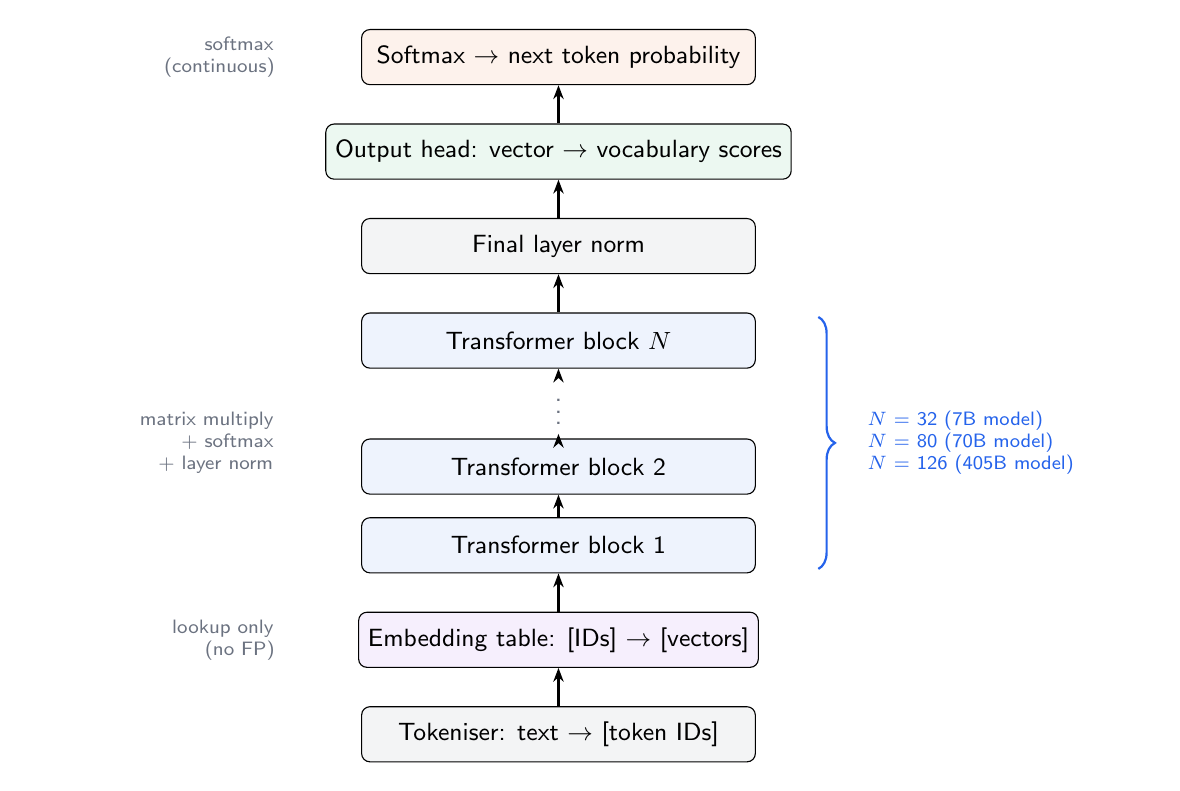
\begin{tikzpicture}[
  comp/.style={draw, rounded corners=3pt, minimum width=5cm,
    minimum height=0.7cm, font=\small\sffamily, align=center},
  arr/.style={-{Stealth[length=5pt]}, thick},
  brace/.style={decorate, decoration={brace, amplitude=6pt, mirror}}
]
  % Stack
  \node[comp, fill=bitgray!8] (tok) at (0, 0)
    {Tokeniser: text $\to$ [token IDs]};
  \node[comp, fill=bitpurple!8] (emb) at (0, 1.2)
    {Embedding table: [IDs] $\to$ [vectors]};
  \node[comp, fill=bitblue!8] (b1) at (0, 2.4)
    {Transformer block 1};
  \node[comp, fill=bitblue!8] (b2) at (0, 3.4)
    {Transformer block 2};
  \node[font=\sffamily, bitgray] (dots) at (0, 4.2) {$\vdots$};
  \node[comp, fill=bitblue!8] (bn) at (0, 5.0)
    {Transformer block $N$};
  \node[comp, fill=bitgray!8] (ln) at (0, 6.2)
    {Final layer norm};
  \node[comp, fill=bitgreen!8] (head) at (0, 7.4)
    {Output head: vector $\to$ vocabulary scores};
  \node[comp, fill=bitorange!8] (sm) at (0, 8.6)
    {Softmax $\to$ next token probability};

  % Arrows
  \draw[arr] (tok) -- (emb);
  \draw[arr] (emb) -- (b1);
  \draw[arr] (b1) -- (b2);
  \draw[arr] (b2) -- (dots);
  \draw[arr] (dots) -- (bn);
  \draw[arr] (bn) -- (ln);
  \draw[arr] (ln) -- (head);
  \draw[arr] (head) -- (sm);

  % Annotations
  \draw[brace, thick, bitblue]
    (3.3, 2.1) -- (3.3, 5.3);
  \node[font=\scriptsize\sffamily, bitblue, right, text width=3.5cm]
    at (3.8, 3.7)
    {$N$ = 32 (7B model)\\$N$ = 80 (70B model)\\$N$ = 126 (405B model)};

  % Operation counts
  \node[font=\scriptsize\sffamily, bitgray, left, text width=3cm,
    align=right] at (-3.5, 1.2) {lookup only\\(no FP)};
  \node[font=\scriptsize\sffamily, bitgray, left, text width=3cm,
    align=right] at (-3.5, 3.7) {matrix multiply\\+ softmax\\+ layer norm};
  \node[font=\scriptsize\sffamily, bitgray, left, text width=3cm,
    align=right] at (-3.5, 8.6) {softmax\\(continuous)};
\end{tikzpicture}
\caption{The complete LLM architecture. Token IDs enter at the bottom,
  pass through $N$ transformer blocks, and produce a probability
  distribution over the next token at the top. The vast majority of
  computation happens in the transformer blocks (middle).}
\label{fig:full-llm}
\end{figure}

\Cref{tab:llm-sizes} shows the scale of modern LLMs.

\begin{table}[htbp]
\centering
\caption{Scale of representative LLMs. Parameter counts determine
  memory requirements; token counts determine the knowledge absorbed
  during training.}
\label{tab:llm-sizes}
\begin{tabular}{@{}lrrrrr@{}}
  \toprule
  \textbf{Model} & \textbf{Params} & \textbf{Layers} & \textbf{$d$}
    & \textbf{Heads} & \textbf{Training tokens} \\
  \midrule
  GPT-2       & 1.5B    & 48  & 1{,}600  & 25  & 40B \\
  Llama 2 7B  & 7B      & 32  & 4{,}096  & 32  & 2T \\
  Llama 2 70B & 70B     & 80  & 8{,}192  & 64  & 2T \\
  Llama 3 405B& 405B    & 126 & 16{,}384 & 128 & 15T \\
  \bottomrule
\end{tabular}
\end{table}

\begin{engineernote}
A 7-billion-parameter model stored in 16-bit floating point requires
$7 \times 10^9 \times 2 = 14$\,GB of memory---just for the weights.
Add activations, key-value cache, and optimizer state, and training
requires 4--8$\times$ more. This is why bitwise models are so
appealing: ternary weights ($\{-1, 0, +1\}$) need only 1.58~bits
per parameter, reducing the 7B model from 14\,GB to under 2\,GB.
\end{engineernote}

% ----------------------------------------------------------------------------
\subsection{Mixture of Experts: Scaling Without Proportional Cost}
\label{sec:moe}
% ----------------------------------------------------------------------------

As models grow larger, a key insight emerged: not every token needs
every parameter. \concept{Mixture of Experts} (MoE) replaces the
single MLP block in each transformer layer with multiple ``expert''
MLPs, and a small \concept{gating network} (also called a router)
decides which experts process each token.

\begin{figure}[htbp]
\centering
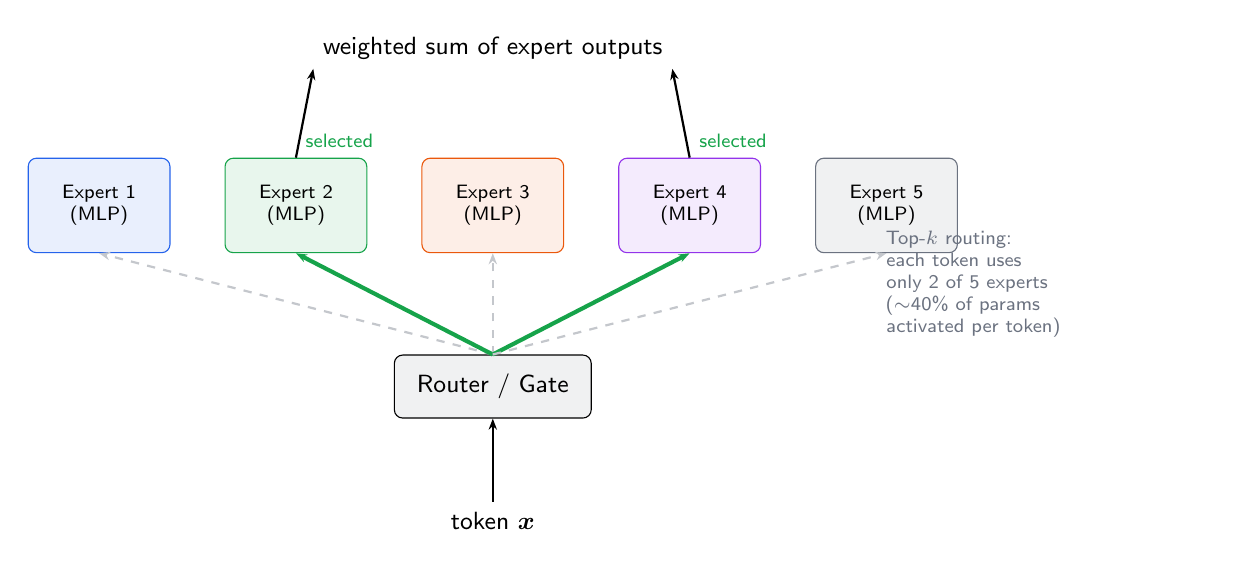
\begin{tikzpicture}[
  expert/.style={draw, rounded corners=3pt, minimum width=1.8cm,
    minimum height=1.2cm, font=\scriptsize\sffamily, align=center,
    fill=#1!10, draw=#1},
  gate/.style={draw, rounded corners=3pt, minimum width=2.5cm,
    minimum height=0.8cm, font=\small\sffamily, fill=bitgray!10},
  arr/.style={-{Stealth[length=4pt]}, thick},
  sel/.style={arr, bitgreen, line width=1.5pt},
  dim/.style={arr, bitgray!40, dashed}
]
  % Input
  \node[font=\small\sffamily] (in) at (5, -0.5) {token $\bm{x}$};

  % Gate
  \node[gate] (g) at (5, 1.2) {Router / Gate};
  \draw[arr] (in) -- (g);

  % Experts
  \node[expert=bitblue]   (e1) at (0,  3.5) {Expert 1\\(MLP)};
  \node[expert=bitgreen]  (e2) at (2.5, 3.5) {Expert 2\\(MLP)};
  \node[expert=bitorange] (e3) at (5,  3.5) {Expert 3\\(MLP)};
  \node[expert=bitpurple] (e4) at (7.5, 3.5) {Expert 4\\(MLP)};
  \node[expert=bitgray]   (e5) at (10, 3.5) {Expert 5\\(MLP)};

  % Gate to experts
  \draw[dim] (g.north) -- (e1.south);
  \draw[sel] (g.north) -- (e2.south);
  \draw[dim] (g.north) -- (e3.south);
  \draw[sel] (g.north) -- (e4.south);
  \draw[dim] (g.north) -- (e5.south);

  % Labels for selected
  \node[font=\scriptsize\sffamily, bitgreen, above right] at (e2.north)
    {selected};
  \node[font=\scriptsize\sffamily, bitgreen, above right] at (e4.north)
    {selected};

  % Output
  \node[font=\small\sffamily] (out) at (5, 5.5)
    {weighted sum of expert outputs};
  \draw[arr] (e2.north) -- (out.south west);
  \draw[arr] (e4.north) -- (out.south east);

  % Annotation
  \node[font=\scriptsize\sffamily, bitgray, text width=4cm, align=left]
    at (12, 2.5) {Top-$k$ routing:\\each token uses\\only 2 of 5 experts\\($\sim$40\% of params\\activated per token)};
\end{tikzpicture}
\caption{Mixture of Experts (MoE). A gating network routes each
  token to the top-$k$ experts (typically $k=2$). The model has many
  parameters (all experts combined) but each token only activates a
  fraction of them, keeping per-token computation manageable.}
\label{fig:moe}
\end{figure}

The gating function is typically a simple linear layer followed by
softmax:
\begin{equation}
  G(\bm{x}) = \text{softmax}(\bm{x}\bm{W}_g)
  \label{eq:gating}
\end{equation}
where $\bm{W}_g \in \mathbb{R}^{d \times E}$ and $E$ is the number
of experts. The top-$k$ values of $G(\bm{x})$ determine which experts
are activated and how their outputs are weighted.

\begin{keyinsight}
MoE decouples \emph{total model knowledge} from \emph{per-token
computation}. A model can have 400B total parameters but only activate
20B per token. This is relevant for bitwise approaches because:
\begin{itemize}[leftmargin=1em]
  \item The router/gating network is a small classification problem
    (``which expert should handle this token?'')---exactly the kind
    of task where Tsetlin Machines or Logic Gate Networks could excel.
  \item Each expert MLP is independent and could be individually
    compiled to logic gates or LUTs.
  \item The ``sparse activation'' principle aligns with bitwise
    networks' strength: small, cache-resident models that run fast.
\end{itemize}
\end{keyinsight}

\begin{analogy}
MoE is like a hospital with specialist departments. A patient (token)
does not see every doctor---a triage nurse (the router) assesses
symptoms and sends them to the relevant specialists. The hospital has
enormous total expertise (parameters), but each patient only uses a
small fraction. This is vastly more efficient than making every doctor
examine every patient.
\end{analogy}

% ----------------------------------------------------------------------------
\subsection{Where the Floating Point Lives}
\label{sec:where-fp-lives}
% ----------------------------------------------------------------------------

Now that we understand the full transformer architecture, we can
precisely identify where floating-point arithmetic is required and
where it might be eliminated. \Cref{tab:fp-map} provides this
breakdown.

\begin{table}[htbp]
\centering
\caption{Floating-point dependency map of a transformer. Recent
  research (I-BERT~\cite{kim2021ibert}, I-ViT~\cite{li2022ivit},
  I-LLM~\cite{hu2024illm}) has demonstrated integer-only
  approximations for components previously thought to require
  floating point.}
\label{tab:fp-map}
\begin{tabular}{@{}p{3.2cm}p{2.5cm}p{6.5cm}@{}}
  \toprule
  \textbf{Component} & \textbf{FP required?} & \textbf{Notes} \\
  \midrule
  Embedding lookup     & No  & Pure table lookup (integer index $\to$ vector). \\
  QKV projection       & Replaceable & Matrix multiply; BitNet uses ternary weights. \\
  $\bm{Q}\bm{K}^\top$ dot product & Replaceable & Integer dot product with ternary weights works. \\
  Softmax              & \textbf{Replaceable} & Integer approximations via polynomial~\cite{kim2021ibert} or bit-shift~\cite{li2022ivit} methods demonstrated. Softmax-free alternatives (linear attention, ReLU attention) also viable. See \cref{sec:softmax-problem}. \\
  Value aggregation    & Replaceable & Weighted sum; integer weights from approximate softmax suffice. \\
  Output projection    & Replaceable & Matrix multiply; can use ternary weights. \\
  Layer normalisation  & \textbf{Replaceable} & Integer RMSNorm via bit-shifting demonstrated in I-ViT and I-LLM~\cite{hu2024illm}. See \cref{sec:layernorm-problem}. \\
  MLP weights          & Replaceable & BitNet uses ternary $\{-1,0,+1\}$. \\
  MLP activation       & Replaceable & LUT-compiled or bit-shift approximation (ShiftGELU~\cite{li2022ivit}). \\
  MoE gating           & Replaceable & Small classification; softmax over few experts. \\
  \bottomrule
\end{tabular}
\end{table}

\begin{keyinsight}
A striking finding from recent research: \emph{every} component in
a transformer has a demonstrated integer-only or bitwise
approximation. The attention softmax can be replaced by polynomial
approximations~\cite{kim2021ibert}, bit-shift
operations~\cite{li2022ivit}, or eliminated entirely in favour of
softmax-free attention mechanisms. Layer normalisation can be
implemented with integer arithmetic and bit-shifts. The question is
no longer ``can we build an integer-only transformer?'' but
``how much accuracy do the combined approximations cost, and can
we close that gap?'' \Cref{sec:scaling-llms} explores this in
detail.
\end{keyinsight}

% ============================================================================
\section{Scaling Bitwise Computation to Large Language Models}
\label{sec:scaling-llms}
% ============================================================================

Armed with an understanding of the transformer architecture, we can
now revisit the question from \cref{sec:hybrid}: can the four bitwise
paradigms be combined in a way that scales to LLM-sized models?

The previous section showed that only two components---the attention
softmax and layer normalisation---fundamentally require floating-point
arithmetic. This section proposes a combination strategy that assigns
each paradigm to the transformer component it is best suited for.

% ----------------------------------------------------------------------------
\subsection{Why No Single Paradigm Scales}
\label{sec:why-no-single}
% ----------------------------------------------------------------------------

Let us first be clear about why each paradigm \emph{alone} fails at
LLM scale:

\begin{description}[leftmargin=1em]
  \item[Binary Neural Networks] can binarise weights and activations,
    but the BNN approach assumes a fixed network topology. It does not
    address the attention mechanism, which is the defining innovation
    of transformers. BitNet b1.58~\cite{ma2024bitnet} succeeds
    precisely because it only binarises the \emph{weights}---not the
    architecture.

  \item[Tsetlin Machines] learn propositional clauses over Boolean
    features. Language tokens are categorical with distributional
    semantics---booleanising 4{,}096-dimensional embeddings would
    destroy the fine-grained similarity structure that makes language
    modelling work. Additionally, Tsetlin Machines have no native
    mechanism for the pairwise token interactions that attention
    provides.

  \item[Logic Gate Networks] with 2-input gates would require
    astronomical circuit depth to approximate the $n \times n$
    attention computation over thousands of tokens. The softmax
    operation is inherently continuous. However, LGNs could work at
    the \emph{component level}---replacing individual MLP blocks
    rather than the entire transformer.

  \item[KAN / LUT compilation] faces an exponential scaling wall:
    lookup tables grow exponentially with input dimensionality.
    A function of 4{,}096-dimensional embeddings cannot be stored
    as a table. But a \emph{univariate} activation function (1D input)
    can easily be stored as a 256-entry table, which is exactly where
    LUT compilation shines.
\end{description}

\begin{keyinsight}
The insight is not ``which paradigm replaces the transformer?'' but
rather ``which paradigm can serve as a component \emph{inside} a
transformer?'' The transformer architecture is non-negotiable for
language. The four paradigms become optimisation techniques within
that structure, not replacements for it.
\end{keyinsight}

% ----------------------------------------------------------------------------
\subsection{A Combined Architecture: Bitwise Components in a Transformer Shell}
\label{sec:combined-architecture}
% ----------------------------------------------------------------------------

We propose mapping each paradigm to the transformer component where
its strengths are most relevant:

\begin{figure}[htbp]
\centering
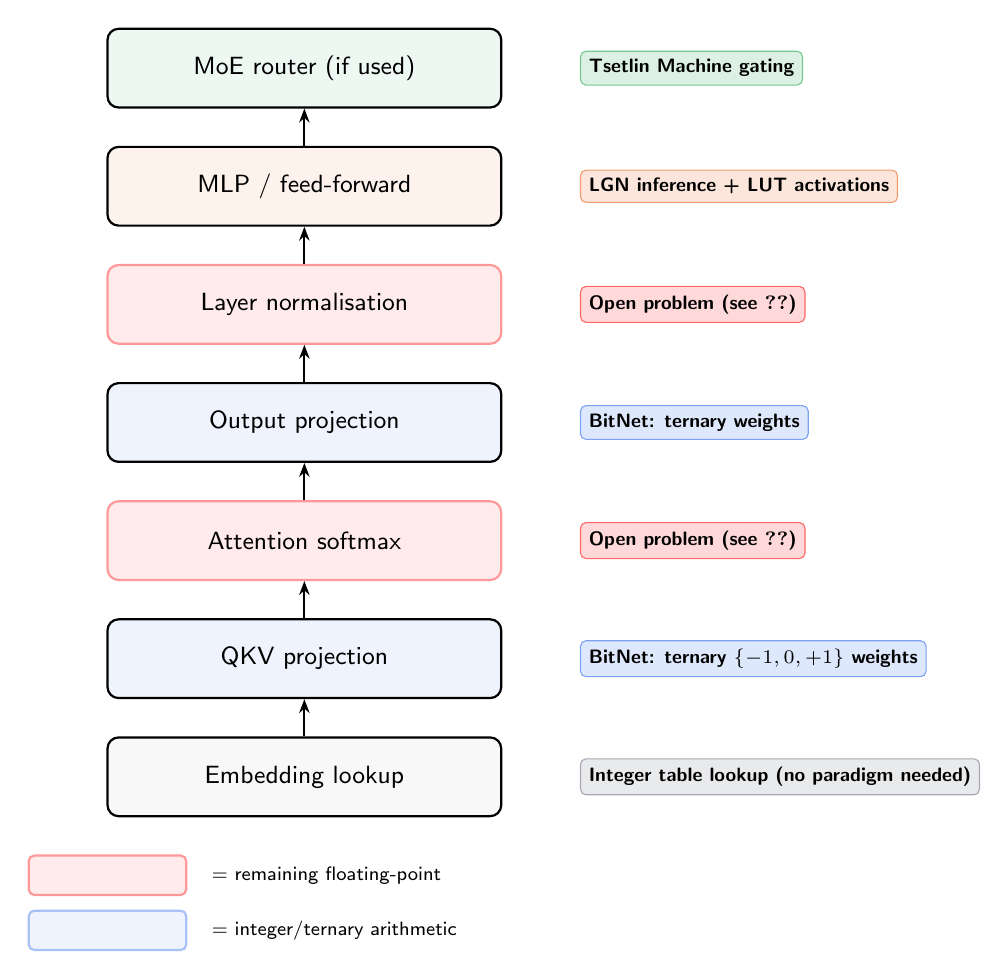
\begin{tikzpicture}[
  comp/.style={draw, rounded corners=4pt, minimum width=5cm,
    minimum height=1.0cm, font=\small\sffamily, align=center,
    line width=0.8pt},
  paradigm/.style={font=\scriptsize\sffamily\bfseries, rounded corners=2pt,
    draw, inner sep=3pt, fill=#1!15, draw=#1!60},
  arr/.style={-{Stealth[length=5pt]}, thick},
  note/.style={font=\scriptsize\sffamily, text width=5cm}
]
  % Components stack
  \node[comp, fill=bitgray!5] (emb) at (0, 0)
    {Embedding lookup};
  \node[comp, fill=bitblue!8] (qkv) at (0, 1.5)
    {QKV projection};
  \node[comp, fill=red!8, draw=red!40] (attn) at (0, 3)
    {Attention softmax};
  \node[comp, fill=bitblue!8] (oproj) at (0, 4.5)
    {Output projection};
  \node[comp, fill=red!8, draw=red!40] (ln) at (0, 6)
    {Layer normalisation};
  \node[comp, fill=bitorange!8] (mlp) at (0, 7.5)
    {MLP / feed-forward};
  \node[comp, fill=bitgreen!8] (gate) at (0, 9)
    {MoE router (if used)};

  % Paradigm labels
  \node[paradigm=bitgray, right] at (3.5, 0)
    {Integer table lookup (no paradigm needed)};
  \node[paradigm=bitblue, right] at (3.5, 1.5)
    {BitNet: ternary $\{-1, 0, +1\}$ weights};
  \node[paradigm=red, right] at (3.5, 3)
    {Open problem (see \cref{sec:softmax-problem})};
  \node[paradigm=bitblue, right] at (3.5, 4.5)
    {BitNet: ternary weights};
  \node[paradigm=red, right] at (3.5, 6)
    {Open problem (see \cref{sec:layernorm-problem})};
  \node[paradigm=bitorange, right] at (3.5, 7.5)
    {LGN inference + LUT activations};
  \node[paradigm=bitgreen, right] at (3.5, 9)
    {Tsetlin Machine gating};

  % Arrows
  \foreach \a/\b in {emb/qkv, qkv/attn, attn/oproj, oproj/ln, ln/mlp, mlp/gate} {
    \draw[arr] (\a) -- (\b);
  }

  % Legend
  \draw[thick, red!40, fill=red!8, rounded corners=2pt]
    (-3.5, -1.5) rectangle (-1.5, -1.0);
  \node[font=\scriptsize\sffamily, right] at (-1.3, -1.25)
    {= remaining floating-point};
  \draw[thick, bitblue!40, fill=bitblue!8, rounded corners=2pt]
    (-3.5, -2.2) rectangle (-1.5, -1.7);
  \node[font=\scriptsize\sffamily, right] at (-1.3, -1.95)
    {= integer/ternary arithmetic};
\end{tikzpicture}
\caption{Proposed mapping of bitwise paradigms to transformer
  components. Green and blue components can be made (near-)bitwise
  today. Red components remain open problems requiring floating-point
  arithmetic or novel replacements.}
\label{fig:combined-architecture}
\end{figure}

\subsubsection{Component 1: BitNet Ternary Weights (BNN Paradigm)}

The weight matrices $\bm{W}_Q$, $\bm{W}_K$, $\bm{W}_V$,
$\bm{W}_O$, $\bm{W}_1$, $\bm{W}_2$ are constrained to ternary
values $\{-1, 0, +1\}$, following the BitNet b1.58
approach~\cite{ma2024bitnet}.

\textbf{What this buys:}
\begin{itemize}[leftmargin=2em]
  \item Weight storage drops from 16~bits to 1.58~bits per parameter
    (a 10$\times$ reduction).
  \item Matrix multiplication becomes addition and subtraction (no
    multiplier circuits needed).
  \item Proven at 3B+ parameter scale with competitive accuracy.
\end{itemize}

\textbf{What remains floating-point:} The activations (intermediate
values flowing between layers) remain in higher precision (typically
8-bit integers in BitNet). The ternary constraint applies only to the
stored weights.

\subsubsection{Component 2: LUT-Compiled Activations (KAN Paradigm)}

The activation functions in the MLP blocks (GELU, SiLU, etc.)
are fixed mathematical functions applied element-wise. Instead of
computing them with floating-point arithmetic, we can:

\begin{enumerate}[leftmargin=2em]
  \item \textbf{Train} with learnable activation functions
    (KAN-style B-splines or learnable piecewise-linear functions).
  \item \textbf{Compile} the learned functions into lookup tables:
    a 256-entry table maps each possible 8-bit input to a
    precomputed output.
\end{enumerate}

\textbf{What this buys:}
\begin{itemize}[leftmargin=2em]
  \item Activation computation becomes a single table lookup---pure
    memory access, no arithmetic.
  \item Each layer can learn its own optimal activation shape, rather
    than using one fixed function everywhere.
  \item The LUT fits in L1 cache (256 entries $\times$ 1~byte = 256~bytes).
\end{itemize}

\textbf{Why KANs do not replace the full MLP:} As discussed in
\cref{sec:ffn}, the MLP block has $d \times d_\text{ff}$ connections.
Replacing each with a full B-spline would create an explosion in
parameters and training cost. But replacing only the
\emph{per-neuron activation function} with a learned spline and then
compiling to a LUT is lightweight and practical.

\subsubsection{Component 3: Logic Gate Network MLP (LGN Paradigm)}

The MLP blocks account for roughly two-thirds of the parameters and
computation in a transformer. After training with ternary weights and
LUT activations, the MLP can potentially be \emph{further compiled}
into a logic gate network for inference:

\begin{enumerate}[leftmargin=2em]
  \item Train the MLP with standard methods (ternary weights + LUT
    activations).
  \item After training, \emph{compile} the trained MLP into an
    equivalent Boolean circuit, where the quantised weights and
    activations are mapped to logic gate configurations.
  \item The inference-time MLP becomes a fixed logic circuit with no
    arithmetic operations.
\end{enumerate}

\textbf{What this buys:}
\begin{itemize}[leftmargin=2em]
  \item Inference-time MLP is pure combinational logic (AND/OR/XOR
    gates)---maximum hardware efficiency.
  \item Maps directly to FPGA or ASIC implementations.
  \item No weight memory needed at inference: the function is
    ``burned into'' the circuit topology.
\end{itemize}

\textbf{What is unproven:} LGNs have been demonstrated at MNIST scale
(thousands of gates). A transformer MLP block at 7B scale has 67M
parameters per layer. Whether the LGN compilation approach can scale
to this size without prohibitive circuit depth or accuracy loss is an
open research question.

\subsubsection{Component 4: Tsetlin Machine Router (TM Paradigm)}

In a Mixture-of-Experts transformer, the gating network decides which
expert processes each token. This is a small classification problem:
given a token's hidden state, select the top-$k$ experts from a pool
of $E$ options.

Tsetlin Machines are a natural fit here because:
\begin{itemize}[leftmargin=2em]
  \item The routing decision is a low-dimensional classification
    (typically $E = 8$ to 64 experts).
  \item The input can be booleanised (e.g., by thresholding the
    hidden state dimensions) without catastrophic information loss,
    because the routing decision does not need the same fine-grained
    precision as the main computation.
  \item The learned clauses would be \emph{interpretable}: we could
    inspect \emph{why} a particular token was routed to a particular
    expert, expressed as human-readable Boolean rules.
\end{itemize}

\textbf{What this buys:}
\begin{itemize}[leftmargin=2em]
  \item Interpretable routing decisions (no black-box gating).
  \item Integer-only routing computation (no floating-point softmax
    in the gating network).
  \item Potential for faster routing than a learned linear layer.
\end{itemize}

\textbf{What is unproven:} Whether Tsetlin Machine routing can match
the load-balancing and accuracy of continuous gating functions at LLM
scale.

% ----------------------------------------------------------------------------
\subsection{The Softmax Problem}
\label{sec:softmax-problem}
% ----------------------------------------------------------------------------

The attention softmax (\cref{eq:softmax}) is the single most
important obstacle to a fully bitwise transformer. Let us examine why
it is hard and what alternatives exist.

\subsubsection{Why Softmax Resists Binarisation}

Softmax converts a vector of raw scores $\bm{z} = [z_1, \ldots, z_n]$
into a probability distribution:

\[
  \text{softmax}(z_i) = \frac{e^{z_i}}{\sum_{j=1}^{n} e^{z_j}}
\]

This operation has three properties that are fundamentally at odds
with bitwise computation:

\begin{enumerate}[leftmargin=2em]
  \item \textbf{Exponentiation.} The function $e^x$ maps integers to
    irrational numbers. There is no bitwise approximation of $e^x$
    that preserves its essential property: amplifying differences
    between large and small values.

  \item \textbf{Normalisation.} Dividing by the sum ensures outputs
    sum to~1. Division is the most expensive basic arithmetic
    operation and does not have a bitwise equivalent.

  \item \textbf{Precision sensitivity.} The attention mechanism
    relies on distinguishing between scores like 0.15 and 0.17. In
    a 4{,}096-token sequence, the softmax distributes attention mass
    across thousands of tokens, and small differences in the
    distribution affect which information propagates forward. Binary
    attention (attend or not) would be too coarse.
\end{enumerate}

\subsubsection{Potential Replacements}

Several research directions aim to reduce or eliminate the softmax:

\begin{description}[leftmargin=1em]
  \item[Linear attention.] Replace $\text{softmax}(\bm{Q}\bm{K}^\top)\bm{V}$
    with $\phi(\bm{Q})\phi(\bm{K})^\top\bm{V}$, where $\phi$ is a
    feature map (e.g., $\text{elu}(x) + 1$ or random
    features). This avoids the $n \times n$ attention matrix entirely.
    Linear attention has $O(n)$ complexity instead of $O(n^2)$, but
    current models using it (e.g., RWKV, Mamba) trade some quality
    for this efficiency.

  \item[ReLU or squared attention.] Replace softmax with
    $\text{ReLU}(\bm{Q}\bm{K}^\top)$ or
    $(\bm{Q}\bm{K}^\top)^2$. These are non-negative (like softmax)
    but avoid exponentiation. Squaring is just multiplication;
    ReLU is a simple threshold (which \emph{is} a bitwise-friendly
    operation). Recent work shows these can achieve competitive
    quality on some tasks, but they lack softmax's normalisation,
    which can cause training instability.

  \item[Integer softmax approximation.] Approximate $e^x$ using
    piecewise linear functions or lookup tables, and approximate
    division using bit shifts. This has been demonstrated in
    inference-only quantisation (e.g., I-BERT), but typically with
    some accuracy degradation.

  \item[Gated attention / state-space models.] Architectures like
    Mamba~\cite{gu2024mamba} and RWKV replace attention entirely
    with recurrent state-space mechanisms that use element-wise
    gating instead of softmax. These are more amenable to
    integer/bitwise implementation, and have shown competitive
    results on language modelling benchmarks at multi-billion
    parameter scale.
\end{description}

\begin{keyinsight}
The softmax problem may not need to be ``solved'' within the
softmax framework. If state-space models (like Mamba) or linear
attention variants prove competitive with transformers at scale,
they offer a path to fully integer attention. The question shifts
from ``how do we binarise softmax?'' to ``can we build LLMs without
softmax at all?'' Early results are promising but not yet
conclusive at the largest scales.
\end{keyinsight}

% ----------------------------------------------------------------------------
\subsection{The Layer Normalisation Problem}
\label{sec:layernorm-problem}
% ----------------------------------------------------------------------------

Layer normalisation (\cref{eq:layernorm}) is the second
floating-point holdout. It requires computing the mean and variance
of a vector, then dividing each element by the standard deviation.

The situation here is more tractable than softmax:

\begin{description}[leftmargin=1em]
  \item[RMSNorm] (used in Llama and most modern LLMs) drops the
    mean computation entirely:
    $\text{RMSNorm}(\bm{x}) = \bm{x} / \text{RMS}(\bm{x}) \cdot \bm{\gamma}$,
    where $\text{RMS}(\bm{x}) = \sqrt{\frac{1}{d}\sum_i x_i^2}$.
    This still requires a square root and division, but the
    computation is simpler.

  \item[Integer RMSNorm.] The sum of squares $\sum_i x_i^2$ is an
    integer operation if $\bm{x}$ is integer. The square root and
    division can be approximated with bit-shift techniques or small
    lookup tables. Practical integer-only implementations have been
    demonstrated in quantised inference.

  \item[BitNet's approach.] BitNet b1.58 retains RMSNorm in
    higher precision, arguing that the normalisation computation is
    a tiny fraction of total operations (it processes $d$ values
    per token, versus $d \times d_\text{ff}$ in the MLP). The
    pragmatic argument: even if normalisation stays in floating
    point, it accounts for less than 1\% of total operations.
\end{description}

\begin{engineernote}
Layer normalisation may be the wrong hill to die on for full
binarisation. Even in a hypothetical ``99\% bitwise'' transformer,
the normalisation steps contribute a negligible fraction of total
energy and latency. The engineering priority should be the
attention mechanism and MLP blocks, which dominate both computation
and memory bandwidth.
\end{engineernote}

% ----------------------------------------------------------------------------
\subsection{The Realistic Picture}
\label{sec:realistic-picture}
% ----------------------------------------------------------------------------

\Cref{tab:bitwise-llm-summary} summarises the current state of each
component.

\begin{table}[htbp]
\centering
\caption{Feasibility assessment for bitwise transformer components.
  ``Proven'' means demonstrated at LLM scale (billions of parameters);
  ``plausible'' means demonstrated at smaller scale or with minor
  accuracy trade-offs; ``open'' means no convincing demonstration
  exists.}
\label{tab:bitwise-llm-summary}
\begin{tabular}{@{}p{3cm}lp{3cm}p{4.5cm}@{}}
  \toprule
  \textbf{Component} & \textbf{Paradigm} & \textbf{Status}
    & \textbf{Key challenge} \\
  \midrule
  Weight storage & BitNet (BNN) & Proven (3B+) & None---ternary weights work. \\
  Matrix multiply & BitNet (BNN) & Proven & Addition/subtraction only. \\
  Activation fn. & KAN $\to$ LUT & Plausible & Per-layer learned activations need validation at scale. \\
  MLP compilation & LGN & Open & Circuit depth at transformer MLP scale. \\
  MoE routing & Tsetlin Machine & Open & Load balancing, accuracy matching. \\
  Attention & (see below) & Open & Softmax replacement. \\
  Layer norm & Integer approx. & Plausible & Small accuracy trade-off acceptable. \\
  \bottomrule
\end{tabular}
\end{table}

\subsubsection{What Could Work Today}

A ``mostly bitwise'' LLM using:
\begin{itemize}[leftmargin=2em]
  \item Ternary weights throughout (BitNet b1.58),
  \item LUT-compiled activation functions,
  \item Integer-approximated RMSNorm,
  \item Standard softmax attention (the remaining floating-point
    component).
\end{itemize}

This configuration would make approximately 95\% of operations
integer or bitwise, with floating point confined to the attention
softmax and a thin normalisation layer. It is achievable with
today's research.

\subsubsection{What Could Work Soon}

Replace softmax attention with a softmax-free alternative:
\begin{itemize}[leftmargin=2em]
  \item State-space models (Mamba) or linear attention for the
    sequence mixing component.
  \item ReLU attention or gated attention as drop-in replacements
    within the transformer structure.
  \item Integer-approximated softmax via LUT-based $e^x$ and
    bit-shift division.
\end{itemize}

This would push the architecture to 99\%+ bitwise/integer operations.
The research exists in pieces; the integration and validation at
scale is the remaining work.

\subsubsection{What Remains Speculative}

A \emph{fully} bitwise LLM with:
\begin{itemize}[leftmargin=2em]
  \item Logic Gate Network MLP blocks (compiled from trained ternary
    MLPs),
  \item Tsetlin Machine MoE routing,
  \item All-integer attention and normalisation.
\end{itemize}

This is the ambitious end-state. Each component exists in isolation
at small scale, but the integration, the compounding of
approximation errors across 80+ layers, and the training dynamics
at billions of parameters are all uncharted territory.

% ----------------------------------------------------------------------------
\subsection{The Path Forward}
\label{sec:path-forward-llms}
% ----------------------------------------------------------------------------

Rather than attempting a fully bitwise LLM immediately, a staged
research programme would build confidence incrementally:

\begin{enumerate}[leftmargin=2em]
  \item \textbf{MNIST hybrid} (current project): Validate the
    four-paradigm combination on a tractable problem.

  \item \textbf{BitNet + LUT activations}: Take an existing BitNet
    model and replace fixed activations with LUT-compiled learned
    activations. Measure accuracy impact. This is a minimal
    intervention with clear evaluation.

  \item \textbf{Softmax-free BitNet}: Combine ternary weights with
    a softmax-free attention mechanism (linear attention, ReLU
    attention, or Mamba-style gating). Evaluate on standard language
    benchmarks.

  \item \textbf{LGN MLP compilation}: Train a small transformer
    (125M parameters) with ternary weights, then attempt to compile
    the MLP blocks into logic gate networks. Measure inference
    speed and accuracy preservation.

  \item \textbf{TM routing for MoE}: Implement Tsetlin Machine
    routing in a MoE transformer and compare with standard softmax
    gating on load balance and accuracy.

  \item \textbf{Integration}: Combine the successful components
    into a single architecture and evaluate at increasing scale.
\end{enumerate}

Each step is independently publishable and valuable regardless of
whether the full vision materialises. The MNIST project we develop
in this article is step~1.

% ============================================================================
\section{Conclusion and Next Steps}
\label{sec:conclusion}
% ============================================================================

\subsection{Summary}

This article has surveyed four paradigms for building neural networks
without traditional multiply-accumulate arithmetic:

\begin{enumerate}[leftmargin=2em]
  \item \textbf{Binary Neural Networks}~\cite{courbariaux2016bnn, rastegari2016xnornet} replace multiplication with
    XNOR and accumulation with popcount. They are the most mature
    paradigm~\cite{bnnsurvey2020}, but CPU performance depends on data
    packing and popcount overhead as well as arithmetic count
    ~\cite{fischer2025popcount}.

  \item \textbf{Tsetlin Machines}~\cite{granmo2018tsetlin} replace the neuron metaphor entirely
    with propositional logic clauses learned through simple automata.
    They are the only paradigm that avoids floating-point arithmetic
    during both training and inference, and they offer full
    interpretability of the learned model. They achieve 99.3\% on
    MNIST~\cite{lecun1998mnist} with the convolutional
    variant~\cite{granmo2019convtm}.

  \item \textbf{Logic Gate Networks}~\cite{petersen2022difflogic} learn both the type and
    connectivity of logic gates end-to-end. New connection-optimised
    training substantially reduces reported gate counts, making them a
    promising sparse Boolean building block rather than merely an
    accelerator-circuit technique~\cite{mommen2026fullytrainable}.

  \item \textbf{KAN/LUT compilation}~\cite{liu2024kan, lutkan2025} trains with maximally expressive
    learnable functions (B-splines on every edge) and then compiles
    them into lookup tables for deployment. This elegantly trades
    memory for computation, achieving near-zero-cost inference at
    the price of larger stored tables.
\end{enumerate}

\subsection{The Hybrid Hypothesis}

We propose a CPU-first search over composable building blocks: Tsetlin
clauses for interpretable sparse features, Logic Gate Networks for learned
Boolean composition, LUTs for small local nonlinearities, and ternary or
low-bit integer kernels where they beat an irregular Boolean graph. A
useful hybrid must achieve competitive accuracy on MNIST while:

\begin{itemize}[leftmargin=2em]
  \item Using \emph{no} floating-point arithmetic at inference time
  \item Producing a partially interpretable model
  \item Using packed CPU operations, local LUTs, and only the low-bit
    arithmetic that materially improves end-to-end runtime
  \item Being implementable in Rust with no external ML framework
    dependencies
\end{itemize}

\subsection{Scaling Beyond MNIST}

\Cref{sec:transformers-llms} and \cref{sec:scaling-llms} examined
whether the bitwise paradigms can scale beyond classification tasks.
The analysis reveals a nuanced picture:

\begin{itemize}[leftmargin=2em]
  \item \textbf{For LLMs:} No single paradigm can replace the
    transformer architecture, but each paradigm can serve as a
    component \emph{within} a transformer. The combination of BitNet
    ternary weights, LUT-compiled activations, Logic Gate Network
    MLP blocks, and Tsetlin Machine MoE routing could yield a
    transformer that is 95--99\% integer/bitwise, with floating point
    confined to the attention softmax and normalisation layers.
    Softmax-free architectures (Mamba, linear attention) offer a
    path to eliminating even that remaining floating-point dependency.

  \item \textbf{For world models and sound synthesis:} The hybrid
    architecture could serve as a fast, interpretable front-end for
    acoustic classification and parameter estimation, feeding into
    classical DSP backends. The KAN/LUT layer is particularly
    promising as a bridge between Boolean features and continuous
    synthesis parameters.
\end{itemize}

\subsection{Next Steps}

\begin{enumerate}[leftmargin=2em]
  \item \textbf{Theory document:} A detailed design document
    specifying the hybrid architecture's mathematical formulation,
    layer dimensions, training algorithm, and convergence properties.

  \item \textbf{Rust implementation:} Implement and benchmark a small
    menu of blocks independently: packed clause masks, SIMD-aware
    binary/ternary dot products, contiguous LGN layers, and cache-sized
    LUT activations. Compose only blocks that beat the same quantised
    integer baseline on the target CPU.

  \item \textbf{Benchmarking:} Systematic comparison against both an
    FP32 MLP and a small quantised integer MLP on accuracy, latency,
    model size, CPU cycles, cache misses, branch behaviour, and energy.

  \item \textbf{Analysis:} Inspection of learned Tsetlin clauses
    for interpretability, gate type distributions in the LGN layer,
    and LUT resolution sensitivity analysis.

  \item \textbf{LLM scaling exploration:} Staged research programme
    from BitNet + LUT activations through softmax-free attention
    to full integration (\cref{sec:path-forward-llms}).
\end{enumerate}

\subsection{A Broader Perspective}

The significance of bitwise neural computation extends beyond any
single task. If these approaches can match floating-point accuracy on
practical problems, they open the door to AI that runs on
microcontrollers, embedded sensors, and edge devices without
specialised hardware---truly democratising access to machine
intelligence.

The honest conclusion is that no single architecture dominates all
tasks. The hybrid approach's strength---everything is Boolean,
interpretable, and cache-resident---is also its constraint. But by
embedding bitwise components within proven architectures (like
transformers) rather than trying to replace those architectures
wholesale, the paradigms surveyed here gain a much broader reach.

The journey from MNIST to fully bitwise language models is long,
but each step along it produces a working, deployable, interpretable
system. That incremental usability may be the hybrid architecture's
most important property.


% --- Bibliography ---
\clearpage
\printbibliography[heading=bibintoc]

\end{document}
